% FEUP THESIS STYLE for LaTeX2e
% how to use feupteses (changed from the original for MIEEC)
%
% FEUP, JCL & JCF, Tue May 20 18:53:15 2008
%
% PLEASE send improvements to jlopes at fe.up.pt, jcf at fe.up.pt
%

%%========================================
%% Commands: pdflatex mieic
%%           bibtex mieic
%%           makeindex mieic (only if crating an index)
%%           pdflatex mieic
%%========================================

%% For one side layout comment next line and uncomment the second line
\documentclass[11pt,a4paper,twoside,openright]{report}
%\documentclass[11pt,a4paper]{report}

%% For iso-8859-1 (latin1), comment next line and uncomment the second line
\usepackage[utf8]{inputenc}
%\usepackage[latin1]{inputenc}

%% Use option portuges if needed
\usepackage[english]{babel}

%% For the final version, comment next line and uncomment the second line
\usepackage[provisional,alpharefs]{feupteses}
%\usepackage[alpharefs]{feupteses}

%% Options:
%% - portuges: titles, etc in portuguese
%% - provisional: the thesis has not been approved yet
%% - usewatermark: use watermark instaed of provisonal text
%% - print: links are not shown (for paper versions)
%% - alpharefs: bibliography references are alphabetic
%% - numericrefs: bibliography references are numbered (in order of citation)
%% ( by default: author-date format of the ``natbib'' package is used
%%   the portuguese version requires the file ``plainnat-pt.bst'' to be
%%   present in the same directory )

%% Include MIEIC definitions different from standard style
\usepackage{mieicpatch}

\usepackage{float}
\usepackage{subfig}

\usepackage{listings}

%% Provide a version number in order to keep track of
%% thesis versions (it will printed in the footer of most pages)

\version{0.99}

%% Uncomment in the final version in order to make version footer disappear
\noversiontrue

%% Uncomment to create an index (at the end of the document)
%\makeindex

%% Path to the figures directory
%% TIP: use folder ``figures'' to keep all your figures
\graphicspath{{figures/}}

%%----------------------------------------
%% TIP: if you want to define more macros, use an external file to
%% keep them
%some macro definitions

% format
\newcommand{\class}[1]{{\normalfont\slshape #1\/}}

% entities
\newcommand{\Feup}{Faculdade de Engenharia da Universidade do Porto}

\newcommand{\svg}{\class{SVG}}
\newcommand{\scada}{\class{SCADA}}
\newcommand{\scadadms}{\class{SCADA/DMS}}

%%----------------------------------------

%%========================================
%% Start of document
%%========================================
\begin{document}

%%----------------------------------------
%% Information about the work
%%----------------------------------------
\title{Improving Variability of Applications using Adaptive Object-Models}
\author{João Gradim Pereira}
\degree{Master in Informatics and Computing Engineering}
%% Date of submission
\thesisdate{17$^{th}$ January, 2011}

%% Insert copyright text if used
%\copyrightnotice{Name of the Author, 2008}

\supervisor{Supervisor}{Ademar Aguiar}{(Ph.D)}
%% Uncomment next line if necessary
\supervisor{Second Supervisor}{Hugo Sereno Ferreira}{(Ph.D AbD)}

%% Uncomment committee stuff in the final version
%\committeetext{Approved in oral examination by the committee:}
%\committeemember{Chair}{Name of the President}{(Title)}
%\committeemember{External Examiner}{Name of the Examiner}{(Title)}
%\committeemember{Supervisor}{Ademar Aguiar}{(Ph.D)}
%\signature
%\committeedate{31$^{st}$ July, 2010}

%% Specify cover logo (in folder ``figures'')
\logo{feup-logo.pdf}

%%----------------------------------------
%% Cover page(s)
%%----------------------------------------
\maketitle

%% Uncomment next line in the final version
\committeepage
%MIEEC uses an external PDF page with the signatures (juri.pdf)
%\includepdf[pagecommand={},noautoscale=false,fitpaper=true,pages=-]{juri.pdf}

%% Preliminary materials
\StartPrelim
\begin{singlespace}
  \chapter*{Abstract}

\chapter*{Resumo}

 % the abstract
  \chapter*{Acknowledgements}

\section*{}

To everyone at \emph{escolinhas.pt}, for making me feel at home throughout all these months.\\
\ \\
To Ademar Aguiar and Hugo Ferreira, for guiding me and for their patience when I had nothing more than questions.\\
\ \\
To Gonçalo and Paulo, for continuously motivating me, supporting my work and helping me whenever I needed.\\
\ \\
To everyone who shared the last 5 and half years with me, night, and day, and then some more.\\
\ \\
To my family, for their undying patience and support, for making me believe in myself and allowing me to be whomever I want to be.\\

\vspace{10mm}
\flushleft{João Gradim}

  % the acknowledgments
  \cleardoublepage
\thispagestyle{plain}

\vspace*{8cm}

\begin{flushright}
   \textsl{``You should be glad that bridge fell down. \\
           I was planning to build thirteen more to that same design''} \\
\vspace*{1.5cm}
           Isambard Kingdom Brunel
\end{flushright}
    % initial quotation if desired
  \cleardoublepage
  \pdfbookmark[0]{Table of Contents}{contents}
  \tableofcontents
  \cleardoublepage
  \pdfbookmark[0]{List of Figures}{figures}
  \listoffigures
  \cleardoublepage
  \pdfbookmark[0]{List of Tables}{tables}
  \listoftables
  \cleardoublepage
  \pdfbookmark[0]{Abbreviations}{abbrevs}
  \chapter*{Abbreviations}
%\addcontentsline{toc}{chapter}{Abbreviations}
\chaptermark{Abbreviations}

\begin{flushleft}
\begin{tabular}{l p{0.8\linewidth}}
PIM       & Platform-Independent Model\\
DSL       & Domain Specific Language\\
RoR       & Ruby on Rails\\
CRUD      & Create, Read, Update, Delete
%ADT      & Abstract Data Type\\
%ANDF     & Architecture-Neutral Distribution Format\\
%API      & Application Programming Interface\\
%CAD      & Computer-Aided Design\\
%CASE     & Computer-Aided Software Engineering\\
%CORBA    & Common Object Request Broker Architecture\\
%UNCOL    & UNiversal COmpiler-oriented Language\\
%Loren    & Lorem ipsum dolor sit amet, consectetuer adipiscing
%elit. Sed vehicula lorem commodo dui\\
%WWW      & \emph{World Wide Web}
\end{tabular}
\end{flushleft}

  % the list of abbreviations used
\end{singlespace}

%%----------------------------------------
%% Body
%%----------------------------------------
\StartBody

%% TIP: use a separate file for each chapter
\chapter{Introduction}\label{chap:intro}

\section{Context}\label{sec:context}

Software systems are usually designed with a specific purpose in mind. They rely on a series of requirements which are often very difficult to capture and maintain, as they have a tendency to evolve faster than the implementation. This is caused mainly by the poor understanding by the stakeholders about their needs and expectations about what a software system should be able to do~\cite{PT07}. These situations lead to higher costs in software development, as creating and maintaining software systems is a knowledge intensive task~\cite{AdOdSBD07}. Moreover, most of these system are not static, and have a constant need to evolve in order to adapt themselves to their environment and new business rules, shifting the stakeholders' needs and expectations about these software systems.

In face of these situations, new development methods started to focus more on iterative and incremental approaches, accepting \emph{incompleteness} as part of every software system development cycle~\cite{WC03}. At the same time, many new systems are being developed with an emphasis on flexibility and run-time configuration~\cite{YJ02}. These approaches present a clear contrast with an up-front, full specification for a software system, which, albeit beneficial for some cases, are impractical in constant evolution scenarios. This leads to a change in software requirements and inevitable refactoring, which in turn may lead to a \textsc{big ball of mud}, ultimately leading to unmaintainable systems, very costly to modify and adapt to the stakeholders needs~\cite{FY97}.

\section{Motivation and Objectives}\label{sec:goals}

Developing quality software is a costly process. Maintaining, as well as adding new features to these software systems is a costly and time-consuming process. If the process of shaping an information system is made to be as streamlined as possible, the modification of the system's architecture (model and relation-wise) becomes a simple task of adapting the platform according to the natural evolution of the business rules, environment changes and the users and stakeholders needs.

The type of systems mentioned in \ref{sec:context} have very specific architectures, which allow for the modification of the system model in runtime. While this may not be desirable in every situation, part of the logic, ideas and patterns of these meta-architectures could be applied to different types of software architectures in order to achieve similar objectives.

Ruby on Rails is one of the most widely used web development frameworks. It provides a series of tools and conventions that allow a developer to focus on the application design rather than implementation details, as most of that work is automatically handled by the framework itself. However, when the kind of aforementioned needs arise in these type of applications, the framework could present itself as a barrier to easily building adaptive software. As such the association of these types of design patterns to a full-stack framework such as Rails presents an interesting challenge --- how to effectively and harmoniously combine these apparently different ideologies to take advantage of the best of both worlds.

This project will be applied to the \textit{Escolinhas}~\cite{escolinhas} project, a growing, Portuguese, Ruby On Rails based project. Escolinhas aims at sustaining social and collaborative work for children in elementary schools involving students, teachers and parents as its users. With the users demanding better and more adaptable teaching tools, it becomes an excellent case-study application to research, test and apply all the work and discoveries made throughout the course of this thesis.

\section{Report Overview}\label{sec:structure}

The rest of this report is structured as follows:\\

\textbf{Chapter \ref{chap:sota}: ``\nameref{chap:sota}'' } reviews the most important methodologies and patterns used to make software as adaptable and maintainable as possible.\\

\textbf{Chapter \ref{chap:problem_statement}: ``\nameref{chap:problem_statement}'' } exposes the problem to be addressed and thoroughly explains it, while explaining it usefulness.\\

\textbf{Chapter \ref{chap:approach_results}: ``\nameref{chap:approach_results}'' } reviews the current design of the platform, and performs a variability analysis of the system, choosing three focus areas. Then, for each one of the areas, demonstrates its variability requirements, candidate patterns, the chosen patterns and rationale behind such decisions, implementation details and impact analysis.\\

\textbf{Chapter \ref{chap:validation}: ``\nameref{chap:validation}'' } validates the work described in Chapter~\ref{chap:approach_results} through various metrics\\ % FIXME

\textbf{Chapter \ref{chap:conclusions}: ``\nameref{chap:conclusions}'' } reviews the project, drawing conclusions about the issues addressed in Chapters \ref{chap:approach_results} and \ref{chap:validation}. It also provides a summary of contributions and some insights on which future developments have been considered.\\


%\chapter{Technologies}\label{chap:technologies}

\section{C\#}\label{sec:csharp}

C\# (C-Sharp) is a multi-paradigm, strongly-typed programming language developed by Microsoft within the .NET framework. C\# is an object-oriented language, but includes support for other programming paradigms such as functional, imperative, and component-oriented. It was built to be a robust and performant language, featuring strong type-checking, array bounds checking, detection of attempts to use uninitialized variables, and automatic garbage collection~\cite{csharp}.

\section{Oghma}\label{sec:oghma}

Oghma is meant to be a reference framework for the development of AOM systems, developed in C\#. It allows the rapid creation of highly variable, dynamic systems. It is currently being developed in the context of the doctoral thesis of Hugo Sereno Ferreira. It is a very complete framework able to create, manage and persist AOM systems, from backend to GUI generation.

Oghma is thus a concrete implementation of a framework based on the reference architecture to develop AOM-based systems established in~\cite{ferreira_phd_2010}, that balances several design and engineering forces. It supports the creation of models resembling MOF~\cite{mof} and UML~\cite{uml}, and aims at covering the entire cycle of system creation and evolution. As an AOM, it allows the introduction of changes to the system during runtime, thus providing a particular kind of confined end-user development.

Furthermore, the framework leverages the infrastructure used to support system evolution to provide additional features, such as auditing over the system’s usage, and time-traveling to an arbitrary point along its evolution (i.e. to set the system in a past state).

Oghma includes a set of interchangeable components designed to have an high degree of flexibility, as it was designed to support several types of persistency engines --- be it in memory or a DBMS.

\section{Ruby}\label{sec:technologies:ruby}

Ruby is a dynamic, purely object oriented programming language, developed by Yukihiro Matsumoto, released in 1995. Ruby supports multiple programming paradigms, including functional, object-oriented, imperative and reflexive. It was inspired by many different languages such as Lisp, Smalltalk, Perl and Ada, and possesses a series of characteristics that make it extremely attractive~\cite{ruby}.


\chapter{State of the Art}\label{chap:sota}

%This chapter will be an overview of these types of approaches and technologies.

\section{Approaches to Creating Adaptable Software}\label{sec:approaches_to_creating_adaptable_software}

There are two main approaches to making systems adaptable: generative programming approaches and meta-architectures.

Generative programming methods approach the adaptability of a system by using an ontological model representative of this system to automatically create executable artifacts or code skeleton than can be further refined according to different needs.

Rails scaffolding and model generation is an excellent example of this approach, which will be further explained in Section \ref{sec:ror}.

On the other hand, systems created with a special architecture designed to adapt at runtime to new user requirements and rules by using descriptive information about the system model that can be interpreted at runtime are sometimes said to possess a ``reflective architecture'' or a ``meta-architecture''~\cite{YBJ01}.

\section{Software Product Lines}\label{sec:spl}

The Software Product Lines (SPL) software development paradigm is promoted as means of reducing time to market, increasing productivity, improving quality and gaining cost effectiveness and efficiency through large-scale reuse~\cite{TC06}. Software product line methods (SPLMs) are practices-based, or plan-driven, software development approaches in which a set of software-intensive systems that share a common, managed set of features are produced from a set of re-usable core assets in a predictive, rather than opportunistic way --- meaning artifacts are only created when the need for their use arises, instead of providing generic, reusable components.

\section{Domain-Driven Design}\label{sec:ddd}

Domain-Driven Design (henceforth referred to as DDD) is a philosophy and way of thinking, first described by Eric Evans in \cite{ddd_book}, aimed at accelerating software projects that have to deal with complicated domains,  with a two-fold premise \cite{ddd_website}:

\begin{itemize}
  \item For most software projects, the primary focus should be on the domain and domain logic; and
  \item Complex domain designs should be based on a model.
\end{itemize}

A third, informal premise is usually associated with DDD, wherein a collaboration between technical domain experts must exist, in order to quickly, over various iterations, reach the core of the problem's concept.

\section{Model-Driven Engineering}\label{sec:mda}

Model-Driven Engineering first appeared in 2001~\cite{Mil03} as an answer to the growing complexity system architectures. This growing complexity and the lack of a integrated view ``forced many developers to implement suboptimal solutions that unnecessarily duplicate code, violate key architectural principles, and complicate system evolution and quality assurance''~\cite{Sch06}.

To address these issues, Model-Driven engineering combines \emph{domain-specific modeling languages} (DSMLs) with \emph{transformation engines} and \emph{generators} in order to generate various types of artifacts, such as source code or alternative model definitions.

The usage of DSMLs ensures that the domain model is perfectly captured in terms of syntax and semantics. This guarantees a flatter learning curve as the concepts present in the language are already known by the domain experts. This also helps a broader range of experts, such as system engineers and experienced software architects, ensure that software systems meet user needs.

The ability to synthesize artifacts from models helps ensure the consistency between application implementations and analysis information associated with functional and quality of service requirements captured by models.

\section{Frameworks}\label{sec:frameworks}

Frameworks provide a series of loosely-coupled components created for a specific purpose that provide generic functionality for the creation of software systems. These components can be overridden or specialized in order to create specific functionality. Frameworks can improve developer productivity and improve the quality, reliability and robustness of new software.  Developer productivity is improved by allowing developers to focus on the unique requirements of their application instead of spending time on application infrastructure. XNA~\cite{xna} and RoR~\cite{rubyonrails} are good examples of popular frameworks that aim to cut development time and costs in very different scenarios.

Frameworks can also be used together with code-generation techniques~\cite{DH04, rails_generators} to improve the overall production speed and ease of use.

\section{Metaprogramming}\label{sec:metaprogramming}

As defined by Robert D. Cameron and M. Robert Ito in~\cite{CI84},

\begin{quote}
 ``A metaprogramming system is a programming facility (subprogramming system or language) whose basic data objects include the programs and program fragments of some particular programming language, known as the target language of the system. Such systems are designed to facilitate the writing of metaprograms, that is, programs about programs. Metaprograms take as input programs and fragments in the target language, perform various operations on them, and possibly, generate modified target-language programs as output.''
\end{quote}

To put it simply, metaprogramming is code that manipulates code. The advantages of this paradigm have been described many times in software reuse literature. The translation of high-level descriptions into low-level implementations (by means of application generators) allows a developer to focus on specification based on tested standards rather than implementation, making tasks like system maintenance and evolution much easier and affordable~\cite{Bas87, Cle88}. %However, the focus of these methodologies is directed to the code level rather than the underlying domain concepts.

\section{Aspect-Oriented Programming}\label{sec:aspect_oriented_programming}

Aspect-Oriented Programming is a programming paradigm that isolates secondary or auxiliary behaviours from the implementation of the main business logic. It has been proposed as a viable implementation of modular crosscutting concerns. Since crosscutting concerns cannot be properly modularized within object-oriented programming, they are expressed as aspects and are composed, or woven, with traditionally encapsulated functionality referred to as components~\cite{KM05, Ste06}. This paradigm has been gaining some momentum particularly because even conceptually simple crosscutting concerns such as tracing during debugging and synchronization, lead to tangling, in which code statements addressing the crosscutting concern become interlaced with those addressing other concerns within the application~\cite{LC03}.

Many AOP implementations work by automatically injecting new code into existing classes (a process which is commonly called \emph{decorating} a class), effectively adding new functionalities that promote extensive code reuse~\cite{Ste06, LC03, metaclass_programming_in_python}.

\section{Design Patterns}\label{sec:design_patterns}

As stated by the architect Christopher Alexander in \cite{christopher_alexander_a_pattern_language}:

\begin{quote}
  ``Each pattern describes a problem which occurs over and over again in our environment, and then describes the core of the solution to that problem, in such a way that you can use this solution a million times over, without ever doing it the same way twice''
\end{quote}

Despite applying the term \emph{design pattern} to architectural problems, it is possible to transpose these ideas to object-oriented design. As such, a design pattern is, to put it simply, a common solution to a recurring problem. \cite{gang_of_four} then defines the four essential components of a design pattern:

\begin{itemize}
  \item The \textbf{Name}, which captures the essence of a design pattern and describes it in as few words as possible (one or two, usually); \\
  \item The \textbf{Problem}, which describes the conditions necessary to apply the pattern, by explaining the problem and its context; \\
  \item The \textbf{Solution}, which describes the elements that make up the design, their relationships, responsibilities, and collaborations, while keeping it as general as possible, so that its application is possible within multiple contexts: \\
  \item The \textbf{Consequences}, which denotes the results and trade-offs pertaining to the application of the pattern, allowing the evaluation of alternative designs and understanding the costs and benefits of applying the pattern. \\
\end{itemize}

\section{Adaptive Object-Models}\label{sec:aom}

Despite all of the advances in the aforementioned areas, most (if not all) the currently used techniques and methodologies still require a programmer or a domain expert in order to modify a system definition and model. A specific type of architecture is required for the end-user to be able to modify part or the entirety of a system to fit the underlying model to their own needs.

As such, an end-user is not expected to have any kind of knowledge about programming, design patterns and system architectures, or about a system of this type comes to be. However, the end-user is sometimes the most knowledgeable part of the development chain, in regards to how the system should behave.

\subsection{AOM Architecture}\label{sec:aom_architecture}

An Adaptive Object-Model pattern is a system architecture that represents classes, attributes, relationships, and behavior as \emph{metadata}. The system definition is based on instances of model abstractions rather than classes. This allows the modification of these model abstractions in runtime to reflect changes in the domain, effectively modifying the system behavior. As a direct consequence, the system instantly reacts to these changes, making it adaptable to change, without the need for recompiling or redeploying~\cite{YBJ01}. This architectural pattern is akin to the Meta Object Facility (MOF), which main purpose is to provide a metadata management and implementation framework. The basic architecture is divided into four tiers, each one compliant with the higher level\cite{mof}, as depicted in Fig.~\ref{fig:aom_mof_levels}:

\begin{figure}[H]
  \centering
  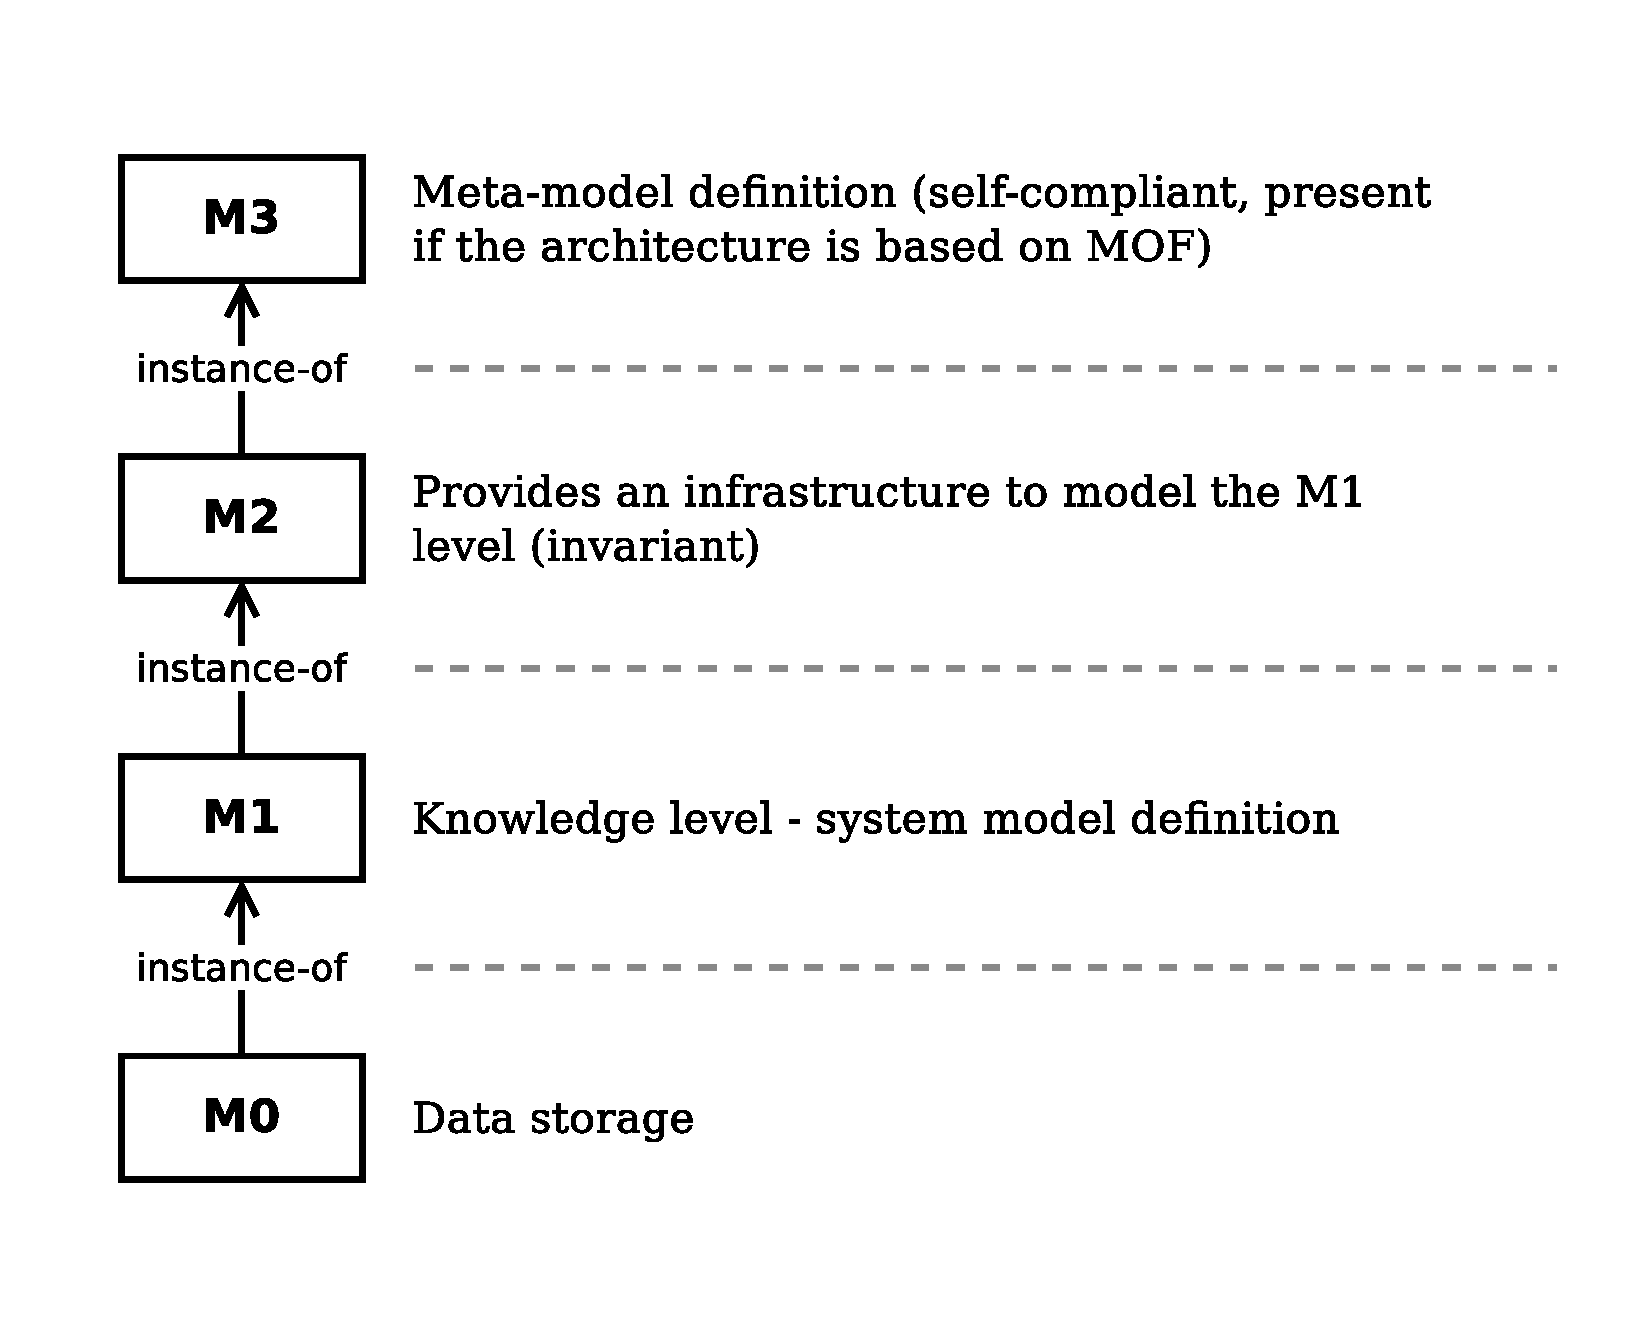
\includegraphics[width=120mm]{aom_mof_levels}
  \caption{MOF levels}
  \label{fig:aom_mof_levels}
\end{figure}

%\begin{itemize}
%  \item M0: Data storage
%  \item M1: Knowledge level --- system model definition
%  \item M2 (invariant): Meta-model --- provides an infrastructure to model the M1 level
%  \item M3 (invariant): Meta-model definition (self-compliant, present if the architecture is based on MOF)
%\end{itemize}

This kind of architecture relies on a series of design patterns: the \textsc{Type-Object} and \textsc{Property} patterns form the basic building blocks whereupon the AOM architecture settles. Despite being extremely simple, they create the fundamental infrastructure able to decouple the model definition from code-level implementation. In addition to these two patterns mentioned, other design patterns which are able to form an AOM architecture will be described, as well as the interactions between them.

\subsubsection{\textsc{Type-Object} Pattern}\label{sec:type-object_pattern}

Object-oriented languages usually structure a program as a set of classes that define the structure and behavior of objects, usually organizing them as a separate class for each object type, which means that any structural change to the model requires code-level modifications. However, variable systems are usually faced with the problem of having a class that will be subclassed by an arbitrary number of specializations. The key to solving this problem is to detach the object definition from the code level and instead define it using meta-data --- generalizing objects and describing their variation as parameters. \textsc{Type-Object} works by splitting a class in two\cite{YBJ01}: the meta-class for the object to be created --- EntityType, and an instance of that class --- Type. Fig. \ref{fig:type-object_pattern} shows the UML class diagram for this design pattern.

\begin{figure}[H]
  \centering
  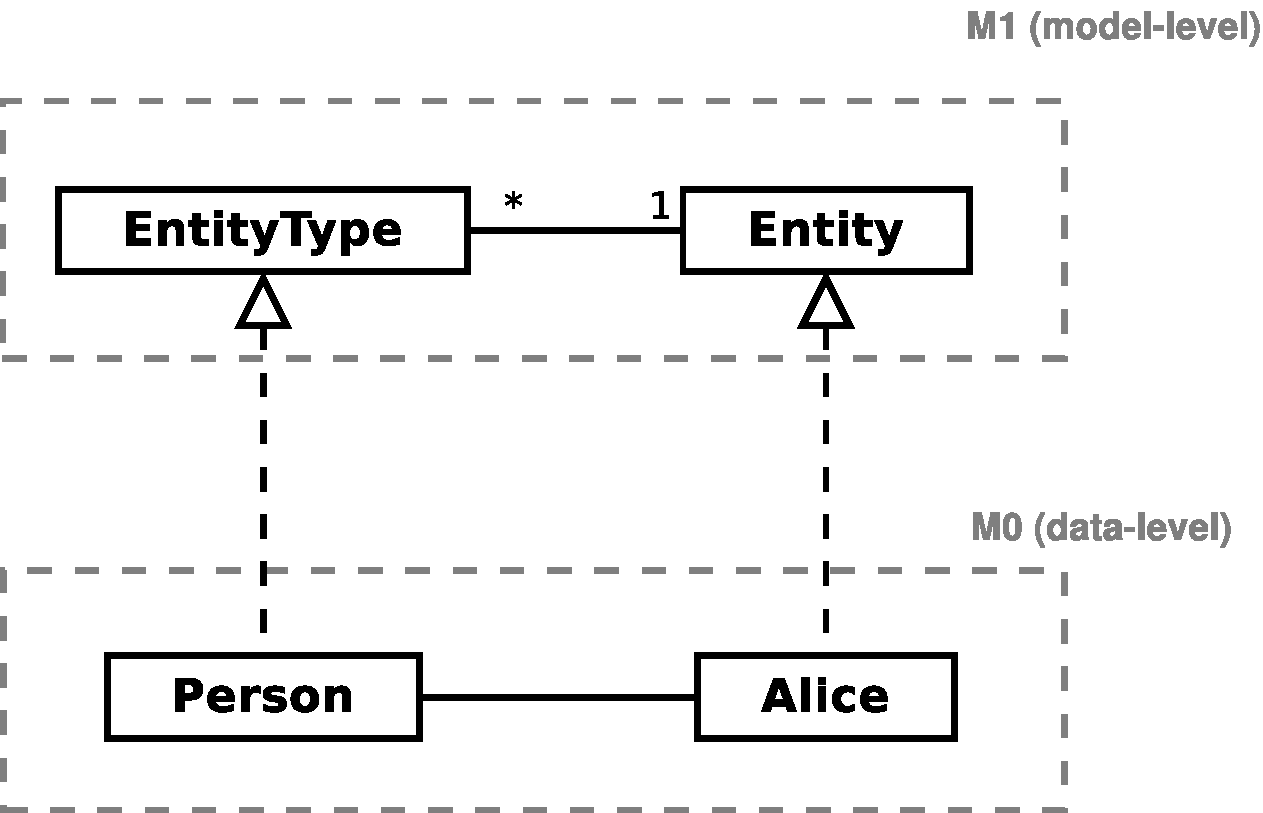
\includegraphics[width=75mm]{type_object.pdf}
  \caption{\textsc{Type-Object} pattern, adapted from \cite{metadata_and_active_object_models}}
  \label{fig:type-object_pattern}
\end{figure}

\subsubsection{\textsc{Property} Pattern}\label{sec:property_pattern}

Similar to the problem solved by the \textsc{Type-Object}, the \textsc{Property} pattern addresses the analogous issues of having the need to change the attributes (sometimes called \emph{members}) of a class. The anticipation of these structural changes leads to the \textsc{Property} pattern, where an attribute is split in two classes: the meta-class for the object to be created --- PropertyType, and an instance of that attribute --- Property. Fig. \ref{fig:property_pattern} represents the UML model for the \textsc{Property} design pattern.

\begin{figure}[H]
  \centering
  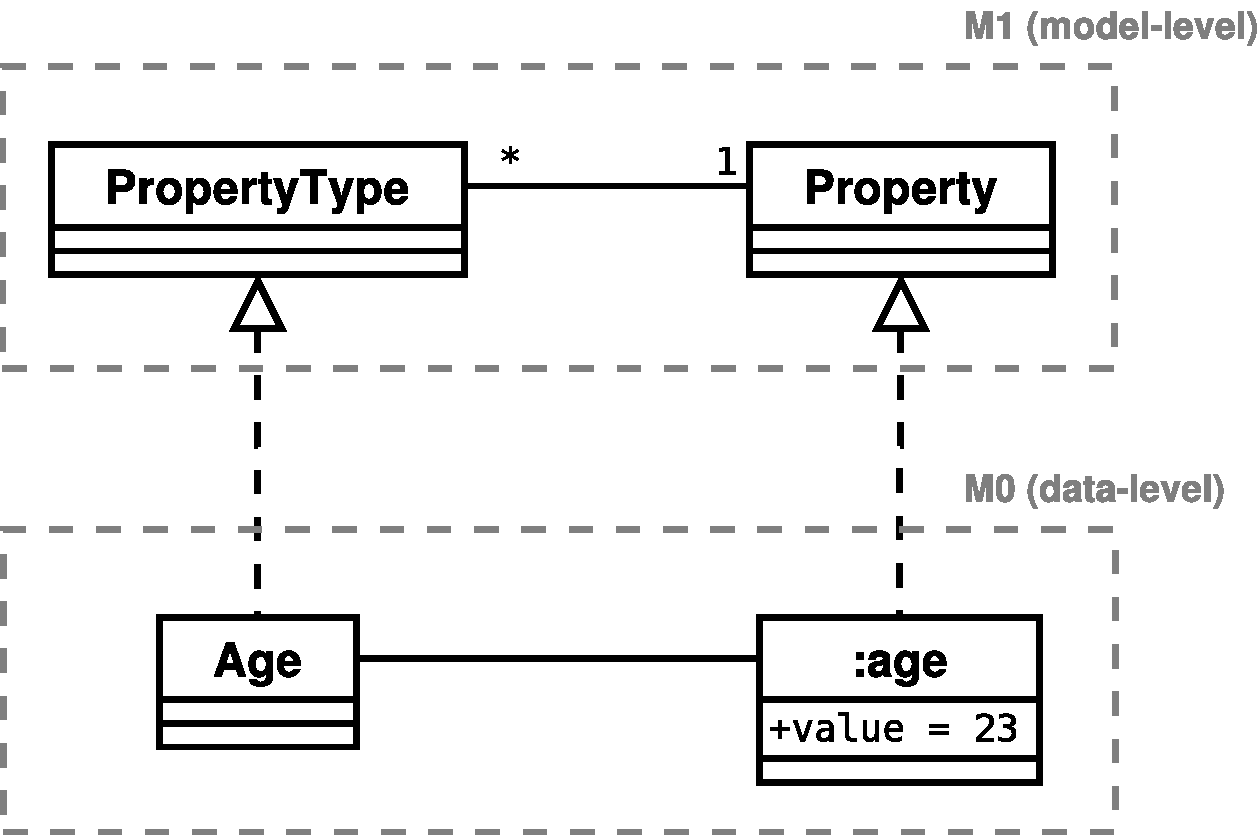
\includegraphics[width=80mm]{property}
  \caption{\textsc{Property} pattern, adapted from \cite{metadata_and_active_object_models}}
  \label{fig:property_pattern}
\end{figure}

\subsubsection{\textsc{Type-Square} Pattern}\label{sec:type-square_pattern}

Usually a class is modeled with a number of different attributes, representing their real world counterparts. So, in order to make a runtime modifiable class, an user must be able to modify both its \emph{definition} and \emph{attributes}. The answer to this issue is to use both \textsc{Type-Object} and \textsc{Property} patterns at the same time, creating what is known as the \textsc{Type-Square} pattern --- which forms the basis of any AOM architecture~\cite{YJ02}. Figure \ref{fig:type_square} shows the UML model for this pattern.

\begin{figure}[H]
  \centering
  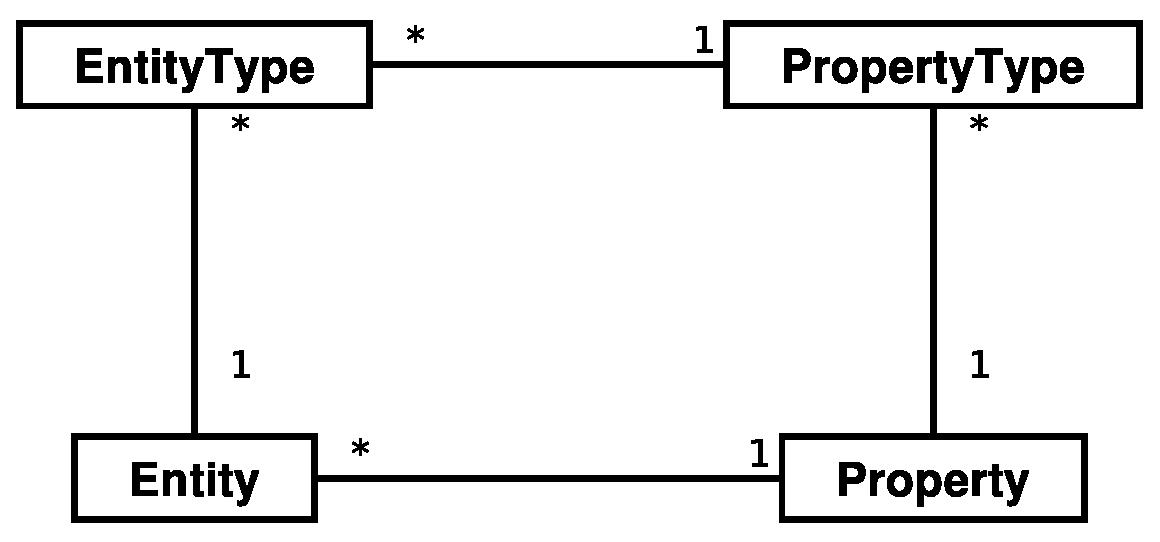
\includegraphics[width=90mm]{type_square}
  \caption{\textsc{Type-Square} pattern, adapted from \cite{YBJ01}}
  \label{fig:type_square}
\end{figure}

\subsubsection{\textsc{Strategy} and \textsc{Rule Object} Pattern}\label{sec:strategy_pattern}

The original goal of the \textsc{Strategy} pattern is to, given a set of algorithms, encapsulate each one in order to use them interchangeably which allows the easy usage of different strategies to solve different problems\cite{gang_of_four}.

As AOM architectures are concerned, this pattern is used to perform user-defined validations for user input, whichever they may be. An example can be found on Fig.~\ref{fig:strategy_pattern}.

\begin{figure}[H]
  \centering
  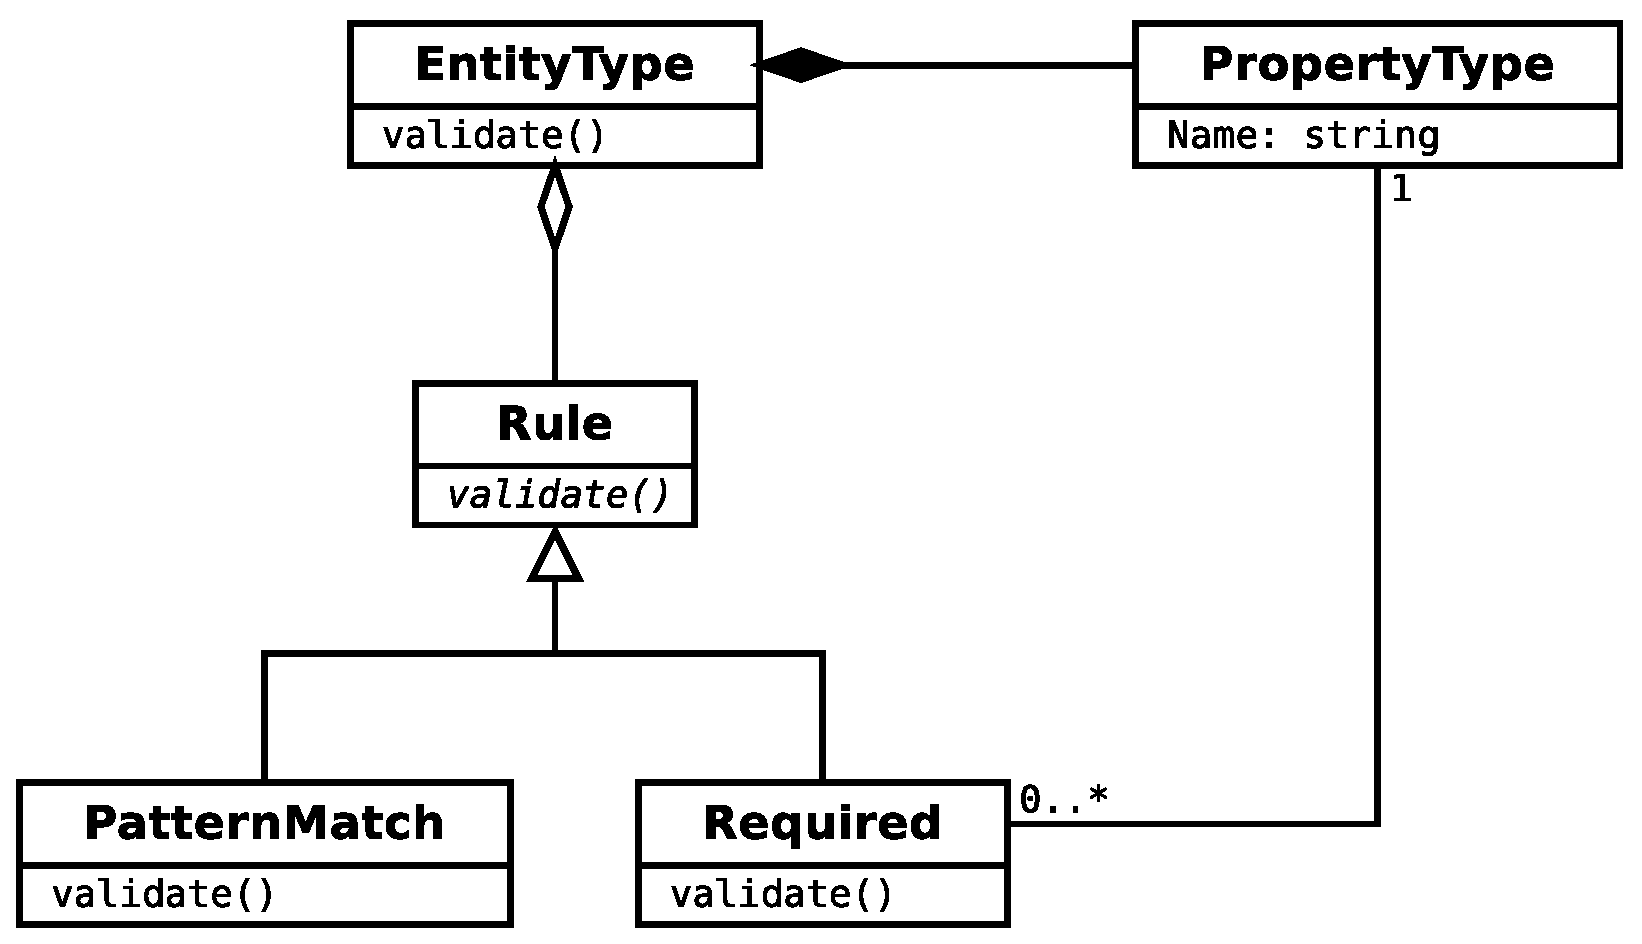
\includegraphics[width=130mm]{strategy}
  \caption{\textsc{Strategy} pattern, as applied to an AOM architecture, adapted from \cite{gang_of_four}}
  \label{fig:strategy_pattern}
\end{figure}

\subsubsection{\textsc{Interpreter} Pattern}\label{sec:interpreter_pattern}

The \textsc{Interpreter} pattern is used when a recurring problem within a platform arises. When this is the case, it might be fruitful to define a simple language to solve these types of problems \cite{gang_of_four}. Regarding AOMs, this pattern, coupled with \textsc{Strategy} (described in \ref{sec:strategy_pattern}), is used to allow users to express complex restrictions on the values of properties present in the system. Fig.~\ref{fig:interpreter_pattern} shows how this pattern is usually applied to AOM architectures, as described in \cite{phd_hugo_ferreira}.

\begin{figure}[H]
  \centering
  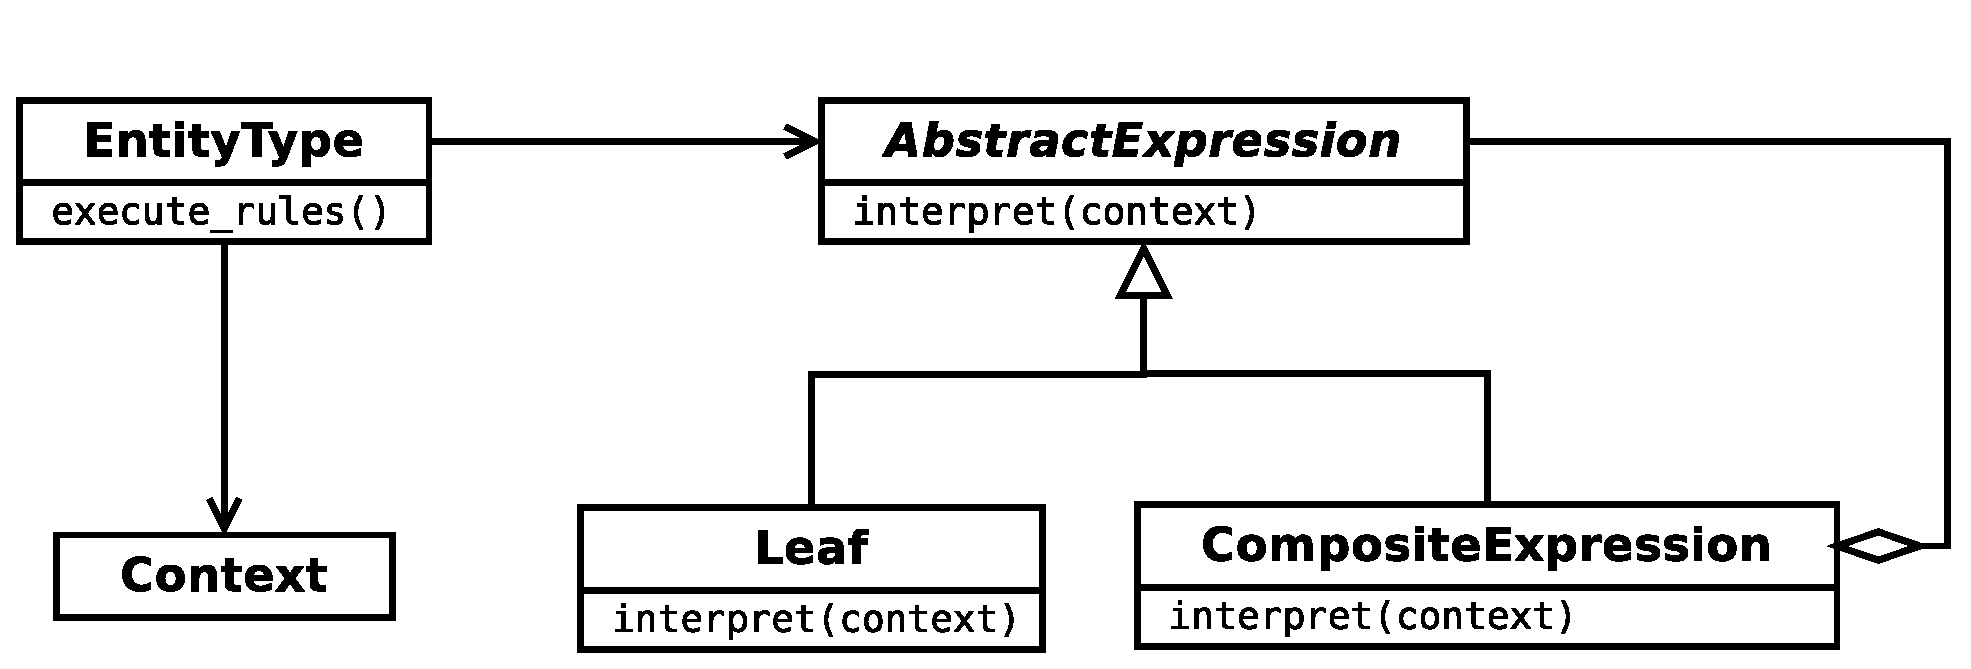
\includegraphics[width=140mm]{interpreter}
  \caption{\textsc{Interpreter} pattern, as applied to an AOM architecture, adapted from \cite{gang_of_four}}
  \label{fig:interpreter_pattern}
\end{figure}

\subsubsection{\textsc{System Memento} Pattern}\label{sec:system_memento_pattern}

The \textsc{System Memento} Pattern is used when one wishes to preserve the different states a system has achieved upon its evolution. The usage of this pattern allows the decoupling of the state from the objects themselves and promotes reusability as the same versioning mechanism can be applied to any entity present in the system. This pattern usually states that an entity in a system (henceforth referred to as a \emph{Thing}) is a composition of \emph{States} (as shown on Fig.~\ref{fig:system_memento}), which, when timestamped, work as evolutionary line for each of the \emph{Things} it is related with. Finally, a \emph{Version} is a collection of all of the \emph{States} in a system, effectively creating a snapshot of the whole system at a given point in time.

\begin{figure}[H]
  \centering
  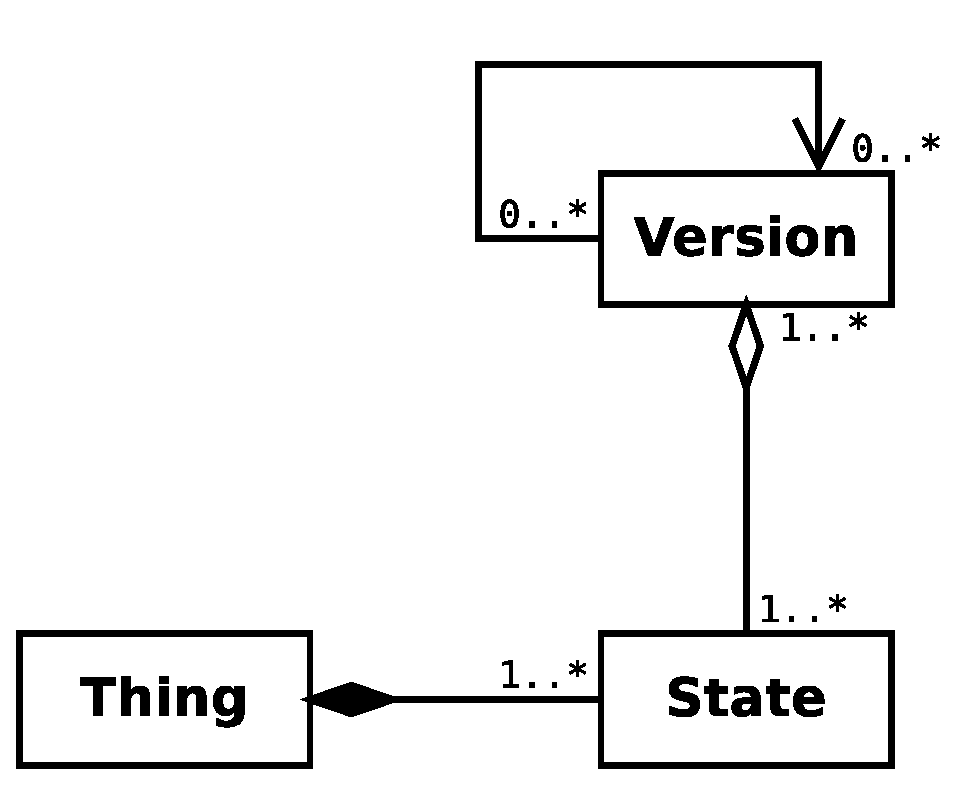
\includegraphics[width=70mm]{system_memento}
  \caption{\textsc{System Memento} pattern, adapted from \cite{patterns_data_and_metadata_evolution_in_aoms}}
  \label{fig:system_memento}
\end{figure}

\subsubsection{Relationships Between Entities}\label{sec:relationships_between_entities}

Yoder \textit{et al.}\cite{YJ02} describes the relationships between AOM classes by using the \textsc{Accountability} pattern~\cite{fowler, hay}. The \textsc{Accountability} pattern is used when there is a need to express multiple types of relationships between \emph{parties} (regardless of what their types may be), all of which carry a different meaning\cite{fowler_accountability}. This pattern is shown on Figure~\ref{fig:accountability}.

\begin{figure}[H]
  \centering
  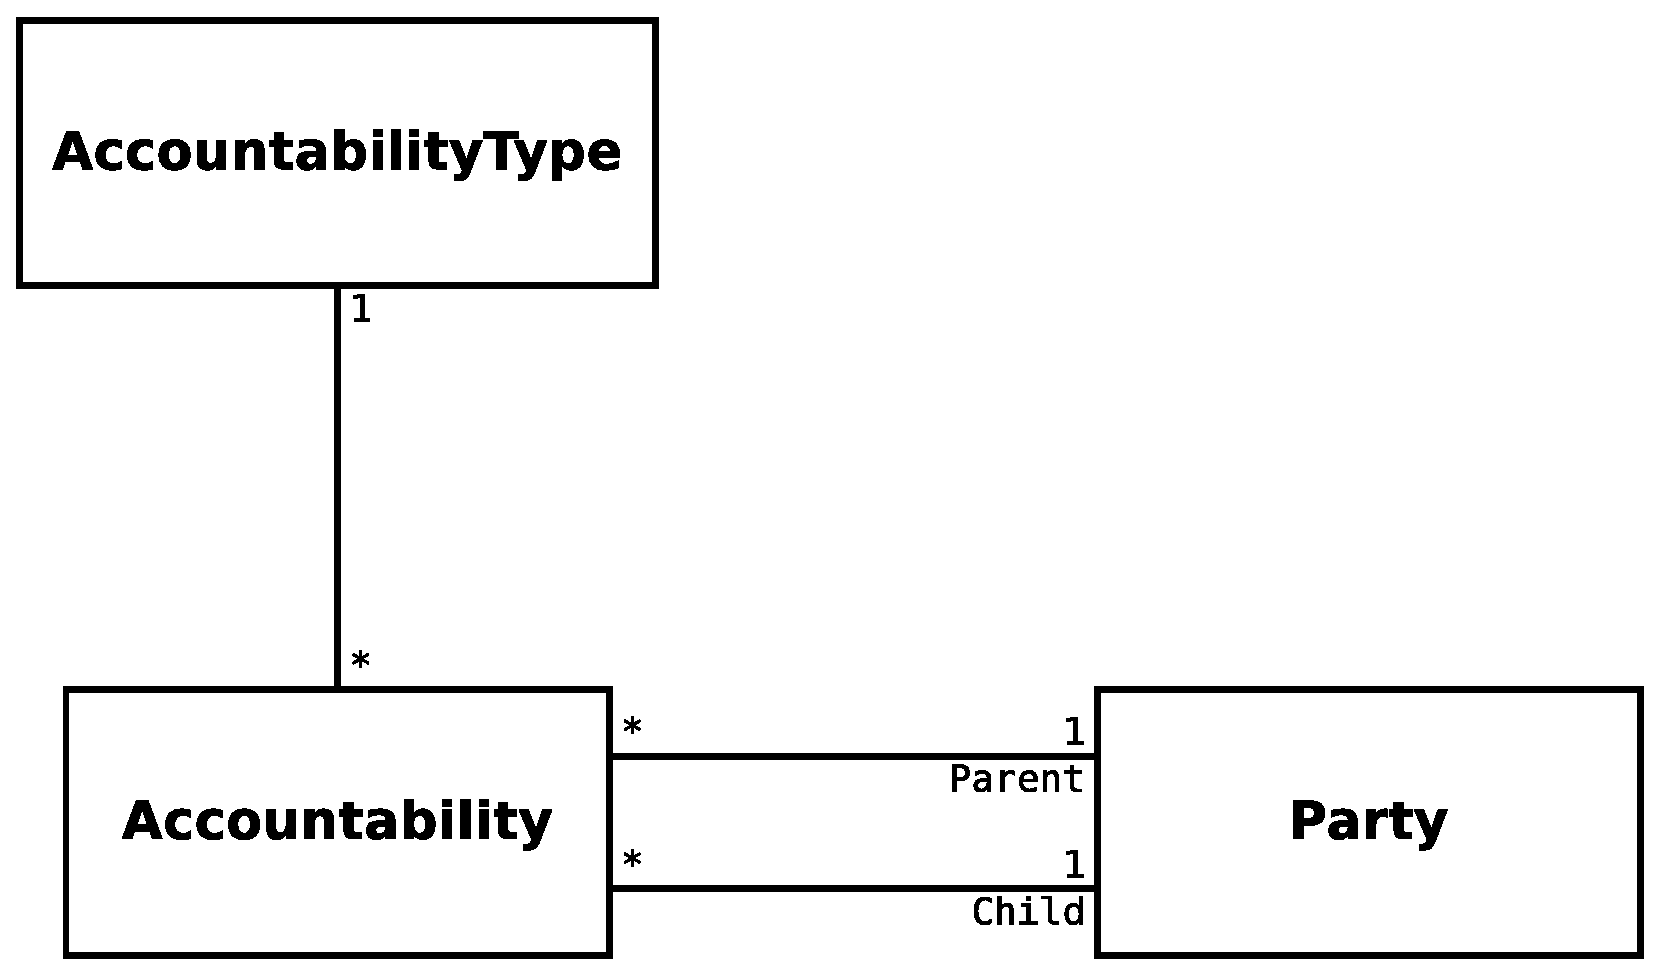
\includegraphics[width=100mm]{accountability}
  \caption{\textsc{Accountability} pattern, adapted from \cite{fowler_accountability}}
  \label{fig:accountability}
\end{figure}

Most OOP languages, however, describe object attributes as either primitive values or references to other objects. Some languages, such as Ruby and Smalltalk, treat everything as an object and do not make any difference between references and primitive values. These concepts can be used to extend the \textsc{Property} pattern, and make it aware of relationships between entities, using attributes such as cardinality, navigability or role~\cite{aom_research_roadmap}.

The revised \textsc{Property} pattern is depicted in Figure \ref{fig:property_revised}:

\begin{figure}[H]
  \centering
  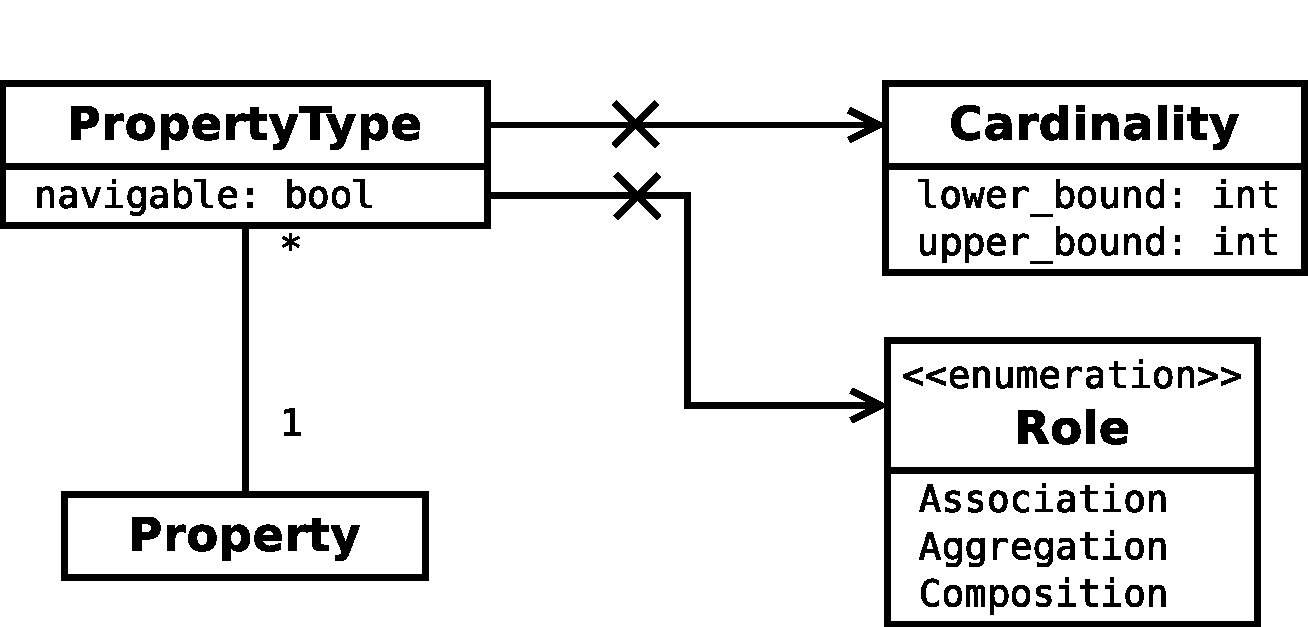
\includegraphics[width=100mm]{property_revised}
  \caption{Revised \textsc{Property} pattern, adapted from \cite{aom_research_roadmap}}
  \label{fig:property_revised}
\end{figure}

\subsection{Pattern Composition}\label{sec:aom_pattern_composition}

By themselves, the design patterns described before do not make up an AOM architecture. Mixing up patterns does not provide any concrete implementation of this kind of architectures, nor it points to what a framework for AOM would look like --- which means that the usual architecture of an AOM is usually the result of composing one or more of the aforementioned patterns in conjunction with other object-oriented patterns. The result of this conjunction can be seen in Fig.~\ref{fig:aom_pattern_composition}

\begin{figure}[H]
  \centering
  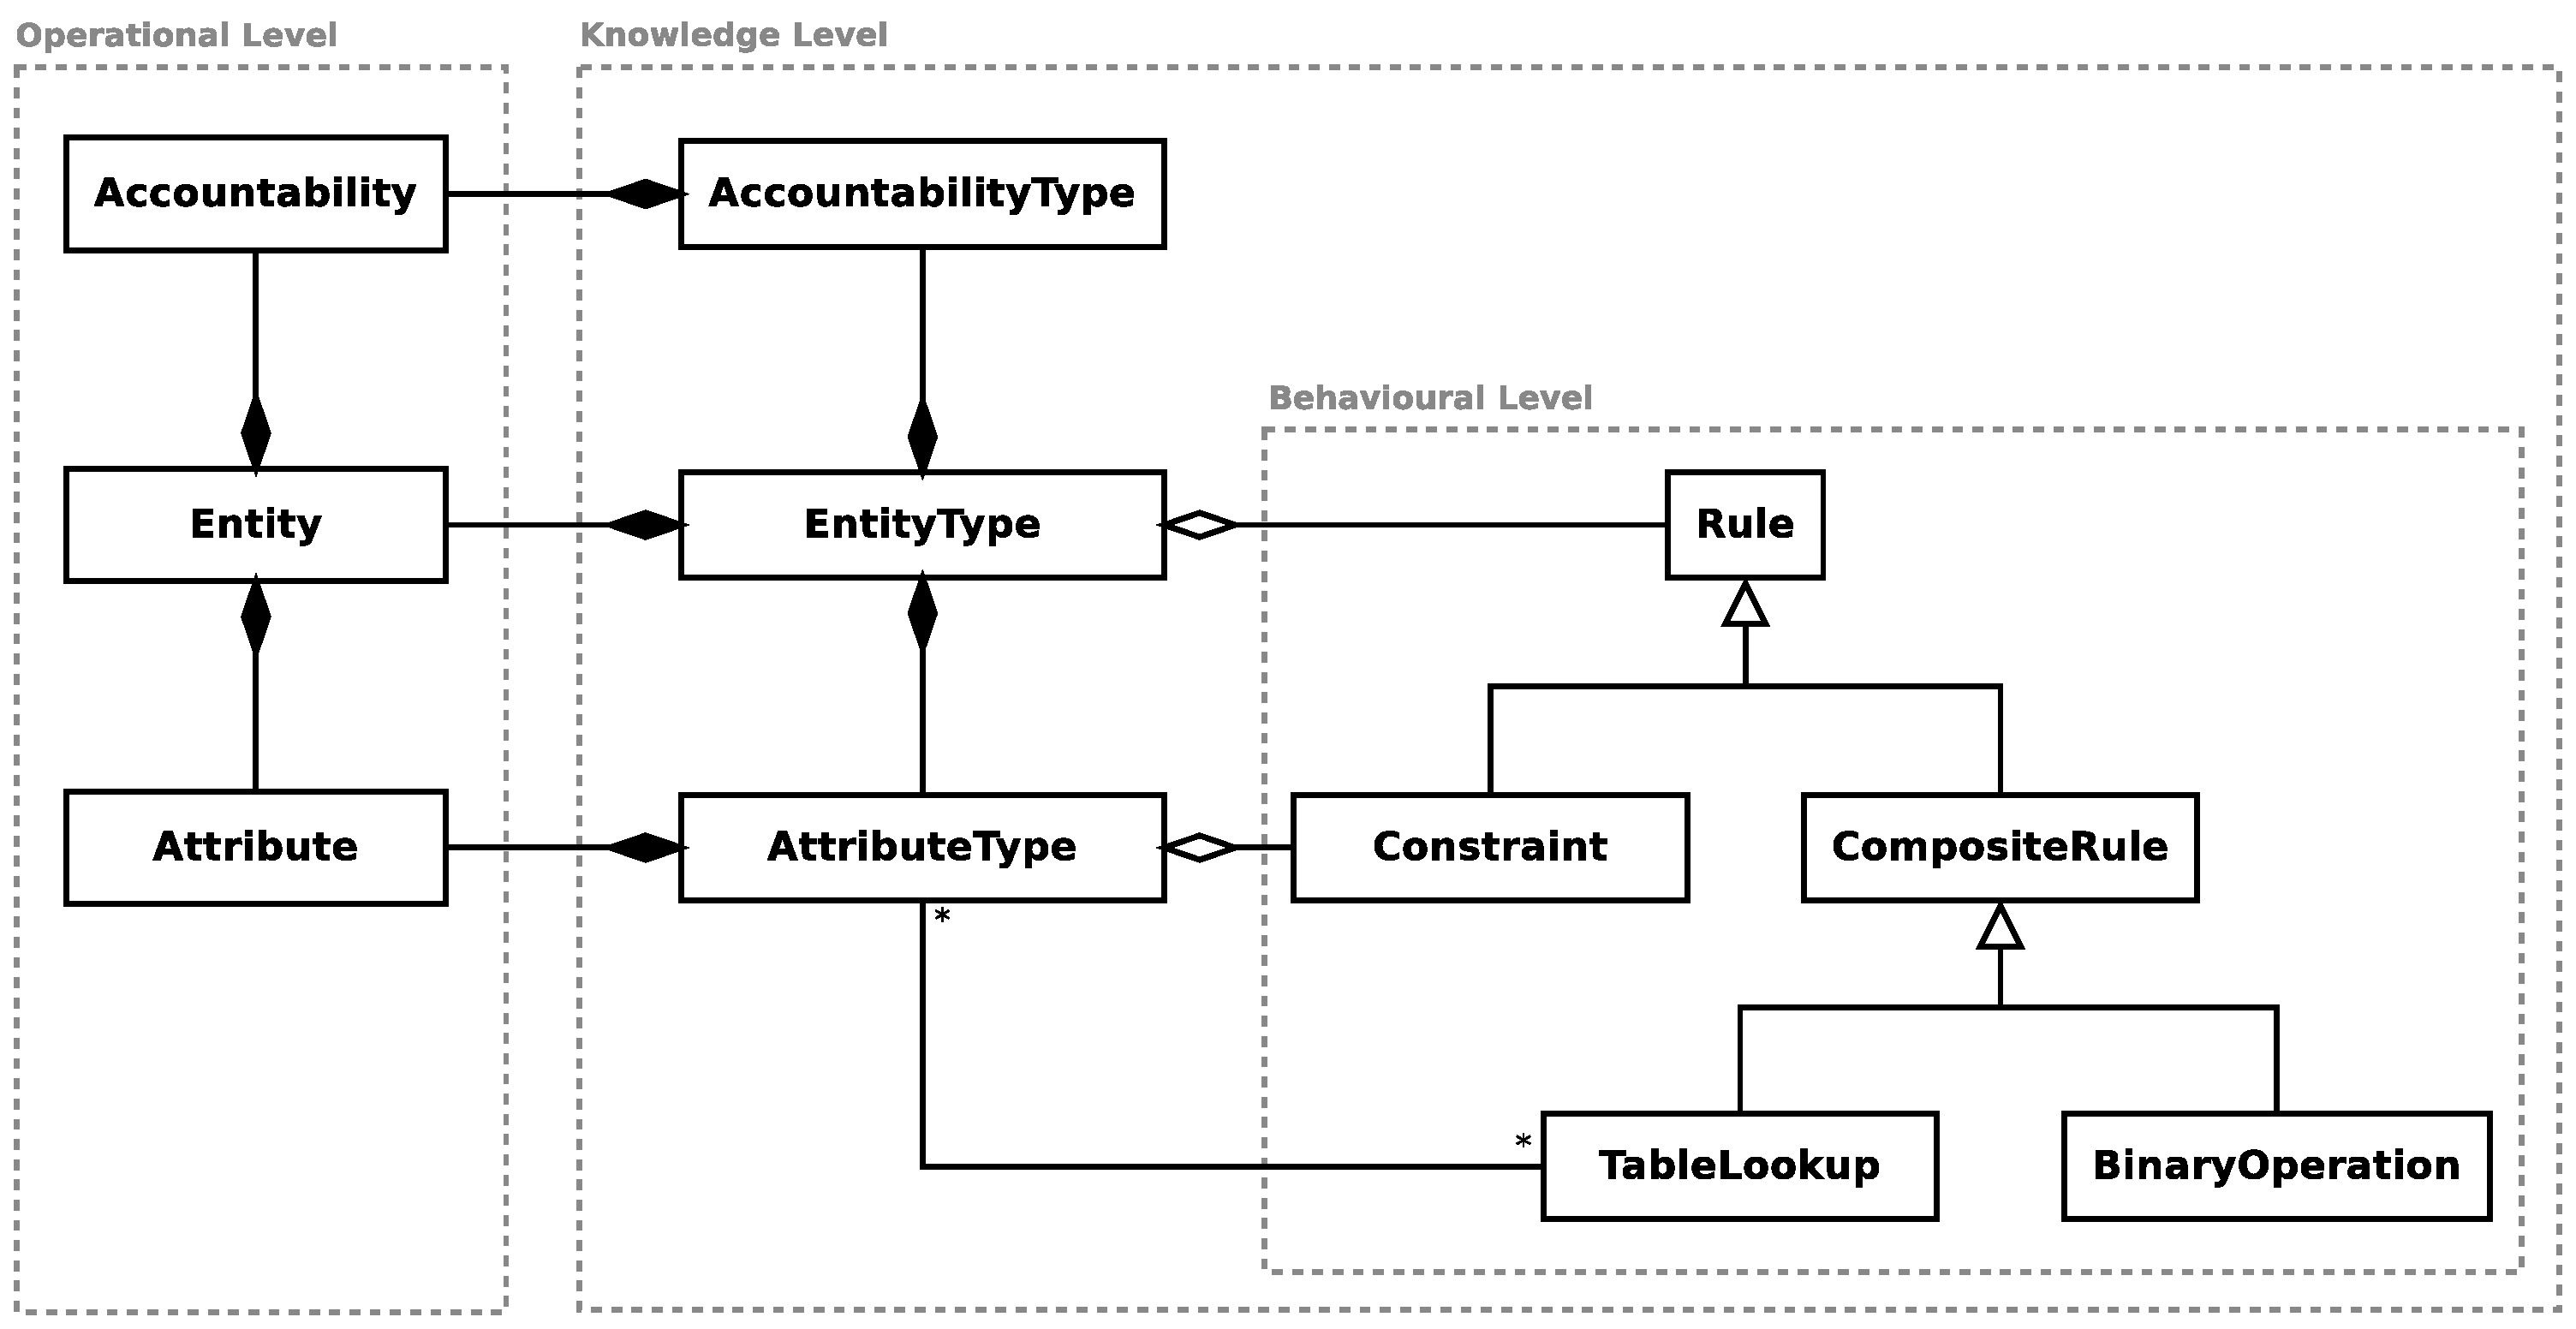
\includegraphics[width=160mm]{aom_pattern_composition}
  \caption{AOM core architecture and design, adapted from \cite{YBJ01}}
  \label{fig:aom_pattern_composition}
\end{figure}

\subsection{AOM GUI Generation}\label{sec:aom_gui_generation}

A system is only as powerful as the interaction with that system allows you to manipulate it --- meaning that a poor interface (be it a GUI or an API or any other kind of interface) does not afford a full-fledged use of the system in question.

Regarding AOM systems, as the system is interpreted and modified in runtime, the GUI must also be automatically built in runtime from the interpretation of the M1 level model. This implies a standardized approach to rendering entities and entity properties, in order to minimize code redundancy and provide a consistent look \& feel. The main problem identified by Welicki et al.\cite{WYW07} was the redundancy that arose from the need to render each type of property, leading to a higher degree of maintenance and potencial UI inconsistency. The solution devised was to create rendering objects responsible for rendering the user interface for each type of property within a given context, creating what is know as the \textsc{Property Renderer} pattern, which enforces a strong separation between domain entities and respective visualization.

However, the separate rendering of single properties is not enough to capture the complexity of an entity. There needs to be a coordination of the various \textsc{Property Renderers} in order to produce a more complex output (be it a UI fragment or a complete interface). The solution is to build view components which coordinate the presentation of several property renderers of an entity to produce different complex UI fragments. Each property renderer is specialized to generate UI code for instances of a property type in a certain context (viewing, editing, different visualization formats, etc). A view component will coordinate several fine-grained renderers and produce more complex UI code for an entity. As such, the same basic concept from \textsc{Property Renderer} can be applied to entities rendering, creating the \textsc{Entity View} pattern~\cite{WYW07}.

\subsection{Oghma}\label{sec:oghma}

Oghma is a reference framework for the development of AOM systems, developed in C\#. It allows the rapid creation of highly variable, dynamic systems. It is currently being developed in the context of the doctoral thesis of Hugo Ferreira. It is a very complete framework able to create, manage and persist AOM systems, from backend to GUI generation, by making extensive use of metaprogramming and metamodeling techniques, by following the general guidelines of the \textsc{Naked Objects} architectural pattern \cite{naked_objects}.

Oghma is thus a concrete implementation of a framework based on the reference architecture to develop AOM-based systems established in~\cite{ferreira_phd_2010}, that balances several design and engineering forces. It supports the creation of models resembling MOF~\cite{mof} and UML~\cite{uml}, and aims at covering the entire cycle of system creation and evolution. As an AOM, it allows the introduction of changes to the system during runtime, thus providing a particular kind of confined end-user development. Fig.~\ref{fig:oghma_core_architecture} show the core architecture for this framework.

It is structured as a collection of \textsc{Layered Component Library} \cite{metaprogramming_metamodeling}, allowing their high-level composition to achieve different functional architectures, e.g. client-server v.s. single-process.

Furthermore, the framework leverages the infrastructure used to support system evolution to provide additional features, such as auditing over the system’s usage, and time-traveling to an arbitrary point along its evolution (i.e. to set the system in a past state).

Oghma includes a set of interchangeable components designed to have an high degree of flexibility, as it was designed to support several types of persistency engines --- be it in memory or a DBMS.

Finally it adds the ability to specify a wide set of behavioural and validation rules by using the \textsc{Interpreter} pattern\cite{gang_of_four}, presenting to the end-user as a  DSL, either through a textual syntax or a graphical interface representative of the rules to be enforced.

\begin{figure}[H]
  \centering
  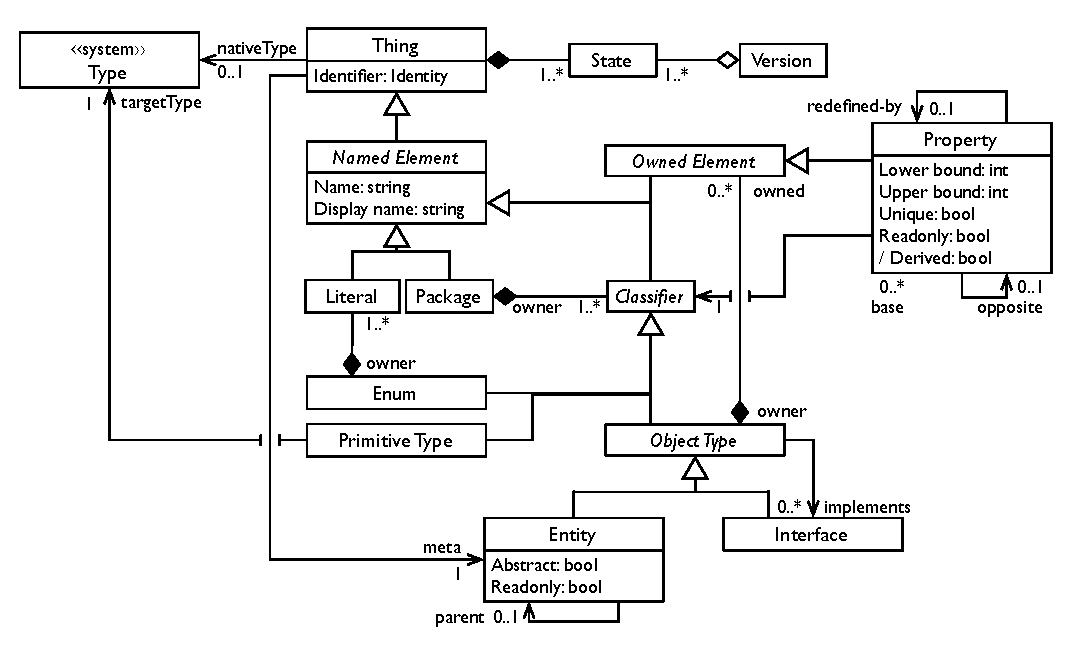
\includegraphics[width=140mm]{oghma_core_architecture}
  \caption{Implementation model of the structural meta-model for the Oghma framework}
  \label{fig:oghma_core_architecture}
\end{figure}

\section{Ruby}\label{sec:ruby}

Ruby is a dynamic, purely object-oriented programming language. It was created by Japanese programmer Yukihiro Matsumoto and it was first released to public in 1995. In its author words, Ruby was created to be a ``a dynamic, open source programming language with a focus on simplicity and productivity. It has an elegant syntax that is natural to read and easy to write''~\cite{ruby}. It was inspired by many different languages such as Lisp, Smalltalk, Perl and Ada, and possesses a series of characteristics that make it extremely attractive~\cite{ruby}.

The Ruby language was designed with a meta-architecture in mind: it allows for changes to class definitions in runtime, constantly adapting to change. It does so by providing open, active class definitions. A common part of the development process when writing a Ruby program is to extend the language by extending the core language classes (such as \verb!String! and \verb!Float!) with custom methods~\cite{metaprogramming_ruby}.

\subsection{Ruby Metaprogramming}\label{sec:ruby_metaprogramming}

Ruby uses metaprogramming techniques extensively --- in fact, metaprogramming is an integral part of some of the language constructs. Take the example from Listing~\ref{fig:ruby_class_metaprogramming}

\begin{lstlisting}[language=ruby, float=htb, label=fig:ruby_class_metaprogramming, caption=Metaprogramming in Ruby classes.]
 class Person
   attr_accessor :name, :age
 end
\end{lstlisting}

The use of the \verb!attr_accessor! declaration is actually a shortcut method for a \emph{getter} and \emph{setter} for the \verb!name! and \verb!age! attributes of the \verb!Person! class. It does so by automatically creating the necessary methods inside a \verb!class_eval! context --- effectively modifying the class definition by evaluating code in runtime. Figure~\ref{fig:ruby_class_metaprogramming_after} represents the code generated internally by the Ruby interpreter when interpreting Listing~\ref{fig:ruby_class_metaprogramming}:

\begin{lstlisting}[language=ruby, float=htb, label=fig:ruby_class_metaprogramming_after, caption=Code generated by Ruby metaprogramming constructs.]
 class Person
   def name=(val)
     @name = val
   end
   def name
     @name
   end
   
   def age=(val)
     @age = val
   end
   def age
     @age
   end
 end
\end{lstlisting}

The usage of the metaprogramming facilities present in Ruby is important in the context of AOM architectures: as a dynamic language, it is able to manipulate and generate code in runtime. This special property of Ruby (and other dynamic languages, such as Python) allows the simplification of many of the patterns described before, especially \textsc{Property} --- by using the capabilities of the language, these patterns are absorbed by the language itself, becoming a normal part of development.

\subsection{Ruby On Rails}\label{sec:ror}

Ruby on Rails is a full-stack Web framework, initially developed by Hansson in 2003, based on the MVC design pattern. As stated by~\cite{rubyonrails}:

\begin{quote}
  ``Ruby on Rails is an open-source that's optimized for programmers happiness and sustainable productivity. It lets you write beautiful code by favoring convention over configuration.''
\end{quote}

In regards to code generation, the Ruby on Rails framework includes a series of mechanisms for system artifacts generation, be it Models, Controllers or even Views. It does so by analyzing the underlying relational database model and deriving the model specifications from the column's type and name. However, RoR does not generate a static model definition, as it deduces the necessary information whenever the system is loaded. Instead, it uses these informations to create an adequate code skeleton for basic CRUD operations in views, greatly accelerating the development process by providing the developers with a basic blueprint of a fully functional system that can be refined and tailored to specific needs~\cite{rails_generators}.

\chapter{Problem Statement}\label{chap:problem_statement}

While Ruby on Rails is built to maximize the developers productivity, it does so by providing a comprehensive set of tools that perform most of the work. The RoR framework is also designed for easy system evolution through \emph{migrations} --- which allow developers to easily add, remove and modify tables and table rows, while minimizing the effort of maintaining application consistency. While this is a solid, proven approach to improve an application's variability over time, it is often less flexible than one might wish, often leading to complicated data migration tasks which may involve modifying production data while ensuring consistency --- this can pose as a problem when the amount of data is extensive and highly variable in nature. As such, the use of a static database schema coupled with migrations may not be entirely desirable for applications highly variable in nature.

As presented on Chapter~\ref{chap:sota}, the usage and application of adequate design patterns is capable of mitigating some of these issues, improving both an application's variability and maintainability.

The main concerns of this thesis are how these architectural and design patterns can be effectively applied to a somewhat (architecturally speaking) restrictive framework, and how these techniques can be combined with a schema-oriented MVC architecture used by the Ruby on Rails Framework. One other point this work is concerned with is how can the variability of such systems increase and how effective they are in terms of development and performance.

\section{Architectural Patterns}\label{sec:architectural_patterns}

The application of architectural patterns is outside the scope of this project, mainly because the project which will serve as a base to the case studies herein described is tied to the Ruby on Rails framework and its implementation of the MVC architecture for software systems. Trying to tackle the problem by changing the underlying architecture would mean that the application would mostly have to be rebuilt from scratch, with the team having to stop development to rewrite the application and learning a whole new set of skills, which is simply not feasible. This process is usually done incrementally and opportunistically, as needs and opportunities appear. Moreover, financial issues would arise from the fact that the escolinhas.pt team would have to be trained in whichever new platform would be used.

\section{Design Patterns}\label{sec:design_patterns}

As the modification of the underlying architecture has been discarded for the reasons stated in \ref{sec:architectural_patterns}, the next step is to try to modify only \emph{parts} of the application design, focusing on a number of different areas --- also known as hotspots --- chosen for their unique requirements in terms of variability. Having chosen these areas, it is important to define which AOM-related design patterns should be applied to solve their problems, and why.

\section{Case-study Areas}\label{sec:case-study_areas}

In order to identify the most adequate areas to focus in, a study of the design of the whole system was necessary --- this allowed the identification of the areas that had naturally occurring highly-variable requirements. For this study, three hotspots within the application were chosen:

\subsection{Roles}\label{sec:case-study_areas_roles}

In escolinhas.pt, a user is associated with a number of different roles. These roles allow to users to perform many different tasks and to have access to a number of distinct sections of the platform --- meaning they are used as the credentials to access and interact with the application. These roles are implemented using a variant of the \textsc{Organization Hierarchy} as described by Martin Fowler in \cite{fowler_accountability}. This implementation leads to a restrictive design, making the task of creating new roles or access rules unnecessarily complicated.
  
\subsection{Social network and contacts}\label{sec:case-study_areas_social_network}
Escolinhas.pt is a social platform for children aged 6 to 10. As such, the network generated by the users is a big part of the application. At this time, this network is built dynamically upon request, by analyzing the relations between users. These relations are derived from the user's school, groups, and friendships. However dynamic, this method proves too restrictive, as there is no convenient and correct way to introduce exceptions in the network --- the only way would be to pollute the code with hard-coded rules. As such, the need for a more flexible system arises.

\subsection{Document Editor}\label{sec:case-study_areas_document_editor}
The document editor present in escolinhas.pt (Fig.~\ref{fig:escolinhas_pt_doc_editor}) is one of the most used parts of the platform. It produces documents which, in their simplest form, have a title and a series of orderable blocks that serve as a placeholder for many different types of content (text, images, drawing, maps, etc). These documents are able to maintain a history of the modifications, in order to audit changes to its content, and to be able to publish a specific version of the document to the platform. While the editor was built with expansibility in mind, the process to create a new type of block is not as streamlined as one may wish. On top of that, the versioning system implemented is very tightly coupled with the \textsc{ActiveRecord} implementation provided by the Ruby on Rails framework, which makes the logic for versioning unnecessarily complicated. This makes the document editor a very interesting area for this kind of study.


\chapter{Approach \& Results}\label{chap:approach_results}

This Chapter presents the main body of work resultant of the study performed for this dissertation, and it is divided in two main parts. The first one is related to research design and it starts by describing how the current design of the \emph{escolinhas.pt} platform was performed and which tools were used to perform said analysis, and how the variability needs for each one of the areas described in \ref{sec:case-study_areas} were identified. The second part describes the development process of each one of the case-study areas: Roles, Social Network and Document Editor. For each one of these areas, it will present the current design and variability requirements. Based on these informations, candidate patterns will be presented, as well as the chosen patterns used to solve the problem and the rationale behind it, outlining why certain patterns were discarded. Then, implementation details will follow, concluding each section with an analysis of the impact each solution had, as well as some results (where applicable).

\section{Research Design}\label{sec:research_design}

The first step taken in order to identify potential problems was to study its current design. This step led to the identification of several points that negatively impacted the variability of the application. After the identification of these points, variability requirements were gathered, so that small, functional prototypes could be built and their impact analyzed within the platform.

\subsection{Current Design Analysis}\label{sec:current_design_analysis}

A thorough analysis of the current design of the application was the first step taken, in order to identify potential problems within the platform. This study was conducted using a series of tools\footnote{Rubymine 2.0 \cite{rubymine} and Rails ERD \cite{rails_erd}} that, unfortunately (at the time of writing), proved unsuccessful in extracting an \emph{Entity Relationship Diagram} from the code of the application --- either they did not work with the current versions of Ruby/Rails used by the platform (Rails ERD) or generated an inaccurate graph. As such, another approach was taken: the product owner of the platform was queried on what he felt were the variability ``hotspots'' of the application: this narrowed the scope of the current design analysis, allowing focus on three different areas, as stated in~\ref{sec:case-study_areas}. These areas were then manually studied --- by analyzing the current database schema, as well as the Model (MVC) source files --- in order to extract the \emph{Entity Relationship Diagrams} relative to each one --- shown ahead on \ref{sec:fa_roles_variability_requirements}, \ref{sec:fa_social_network} and \ref{sec:fa_documents} --- which allowed analyzing each one as independently as possible, so that the applied design patterns (if any) would emerge --- making the task of pinpointing exactly what was wrong with each approach much easier.

\subsection{Variability Analysis}\label{sec:variability_analysis}

Each one of the areas --- Roles, Social Network and the Document Editor --- referred in \ref{sec:case-study_areas} was then studied in order to determine their variability requirements, and to which degree this variability should exist: developer, system administrator, or even end-user. These requirements were defined by the carefully considering the opinions from the users of the platform, the product owner and the main developers. These requirements were then used to determine which design patterns would be more appropriate to achieve the problems posed by each of the areas, and why.

\subsection{Implementation \& Impact Analysis}

For each one the three focus areas, functional prototypes were developed, either directly on top of the platform (Social Network, \ref{sec:fa_social_network}, and User Roles, \ref{sec:fa_roles}) or as an independent proof-of-concept application (Document Editor, \ref{sec:fa_documents}), that, as soon as possible, will be integrated into the main platform. These prototypes, however simplistic (and not yet in production), will be able to validate the research and decisions made throughout the next sections. All of the prototypes are implemented using Ruby 1.9.1 and Rails 2.3.9, as used in the production and development environments of \emph{escolinhas.pt}.

The impact analysis for each of these areas will be made in two different fronts: variability and performance. Variability impact analysis will be concerned with the increase in flexibility/configurability of a certain component, and how it measures to the objectives established beforehand. Performance analysis will (if applicable) examine the how much more (or less) performant each one of the implementations is, compared to the previous solutions.

\section{Development}\label{sec:development}

After studying the current design of the application and collecting the necessary requirements, the development phase took place: the major variability requirements were outlined, and a set of design patterns carefully considered, with their benefits and disadvantages weighed in order to correctly choose the most appropriate solution. Finally, proof-of-concept prototypes were built so that the choice of patterns could be validated and the impact resultant from said implementations measured.

\subsection{User Roles}\label{sec:fa_roles}

Roles play a very important part in any application: by attaching them to users, they allow the application to authenticate and authorize users based on their roles. If an application has a strong tendency to evolve, so do its roles and authorization sets. This section describes the work involved in making the current system of roles used in \emph{escolinhas.pt} as adaptable as possible.

\subsubsection{Variability Requirements}\label{sec:fa_roles_variability_requirements}

Authorization is one of the most sensitive areas of any closed software system: it ensures everyone does only what it should in order to guarantee everything works as expected. In a constantly evolving system, the accesses granted by user roles have a tendency to shift and evolve alongside the application --- either because of new features or a new type of user is required in the system to perform specific tasks. In the context of \emph{escolinhas.pt} this problem ties itself with the ACL used: because of the diversity of roles (Fig.~\ref{fig:user_roles_current}) and the three different usage plans, a lot of different rules are applied to determine if a user can or can not perform certain actions; allied to the growing number of features of the platform, this means that the authorization scheme has to be as flexible as possible to ensure minimal overhead when determining new types of permission sets.

\begin{figure}[h]
  \centering
  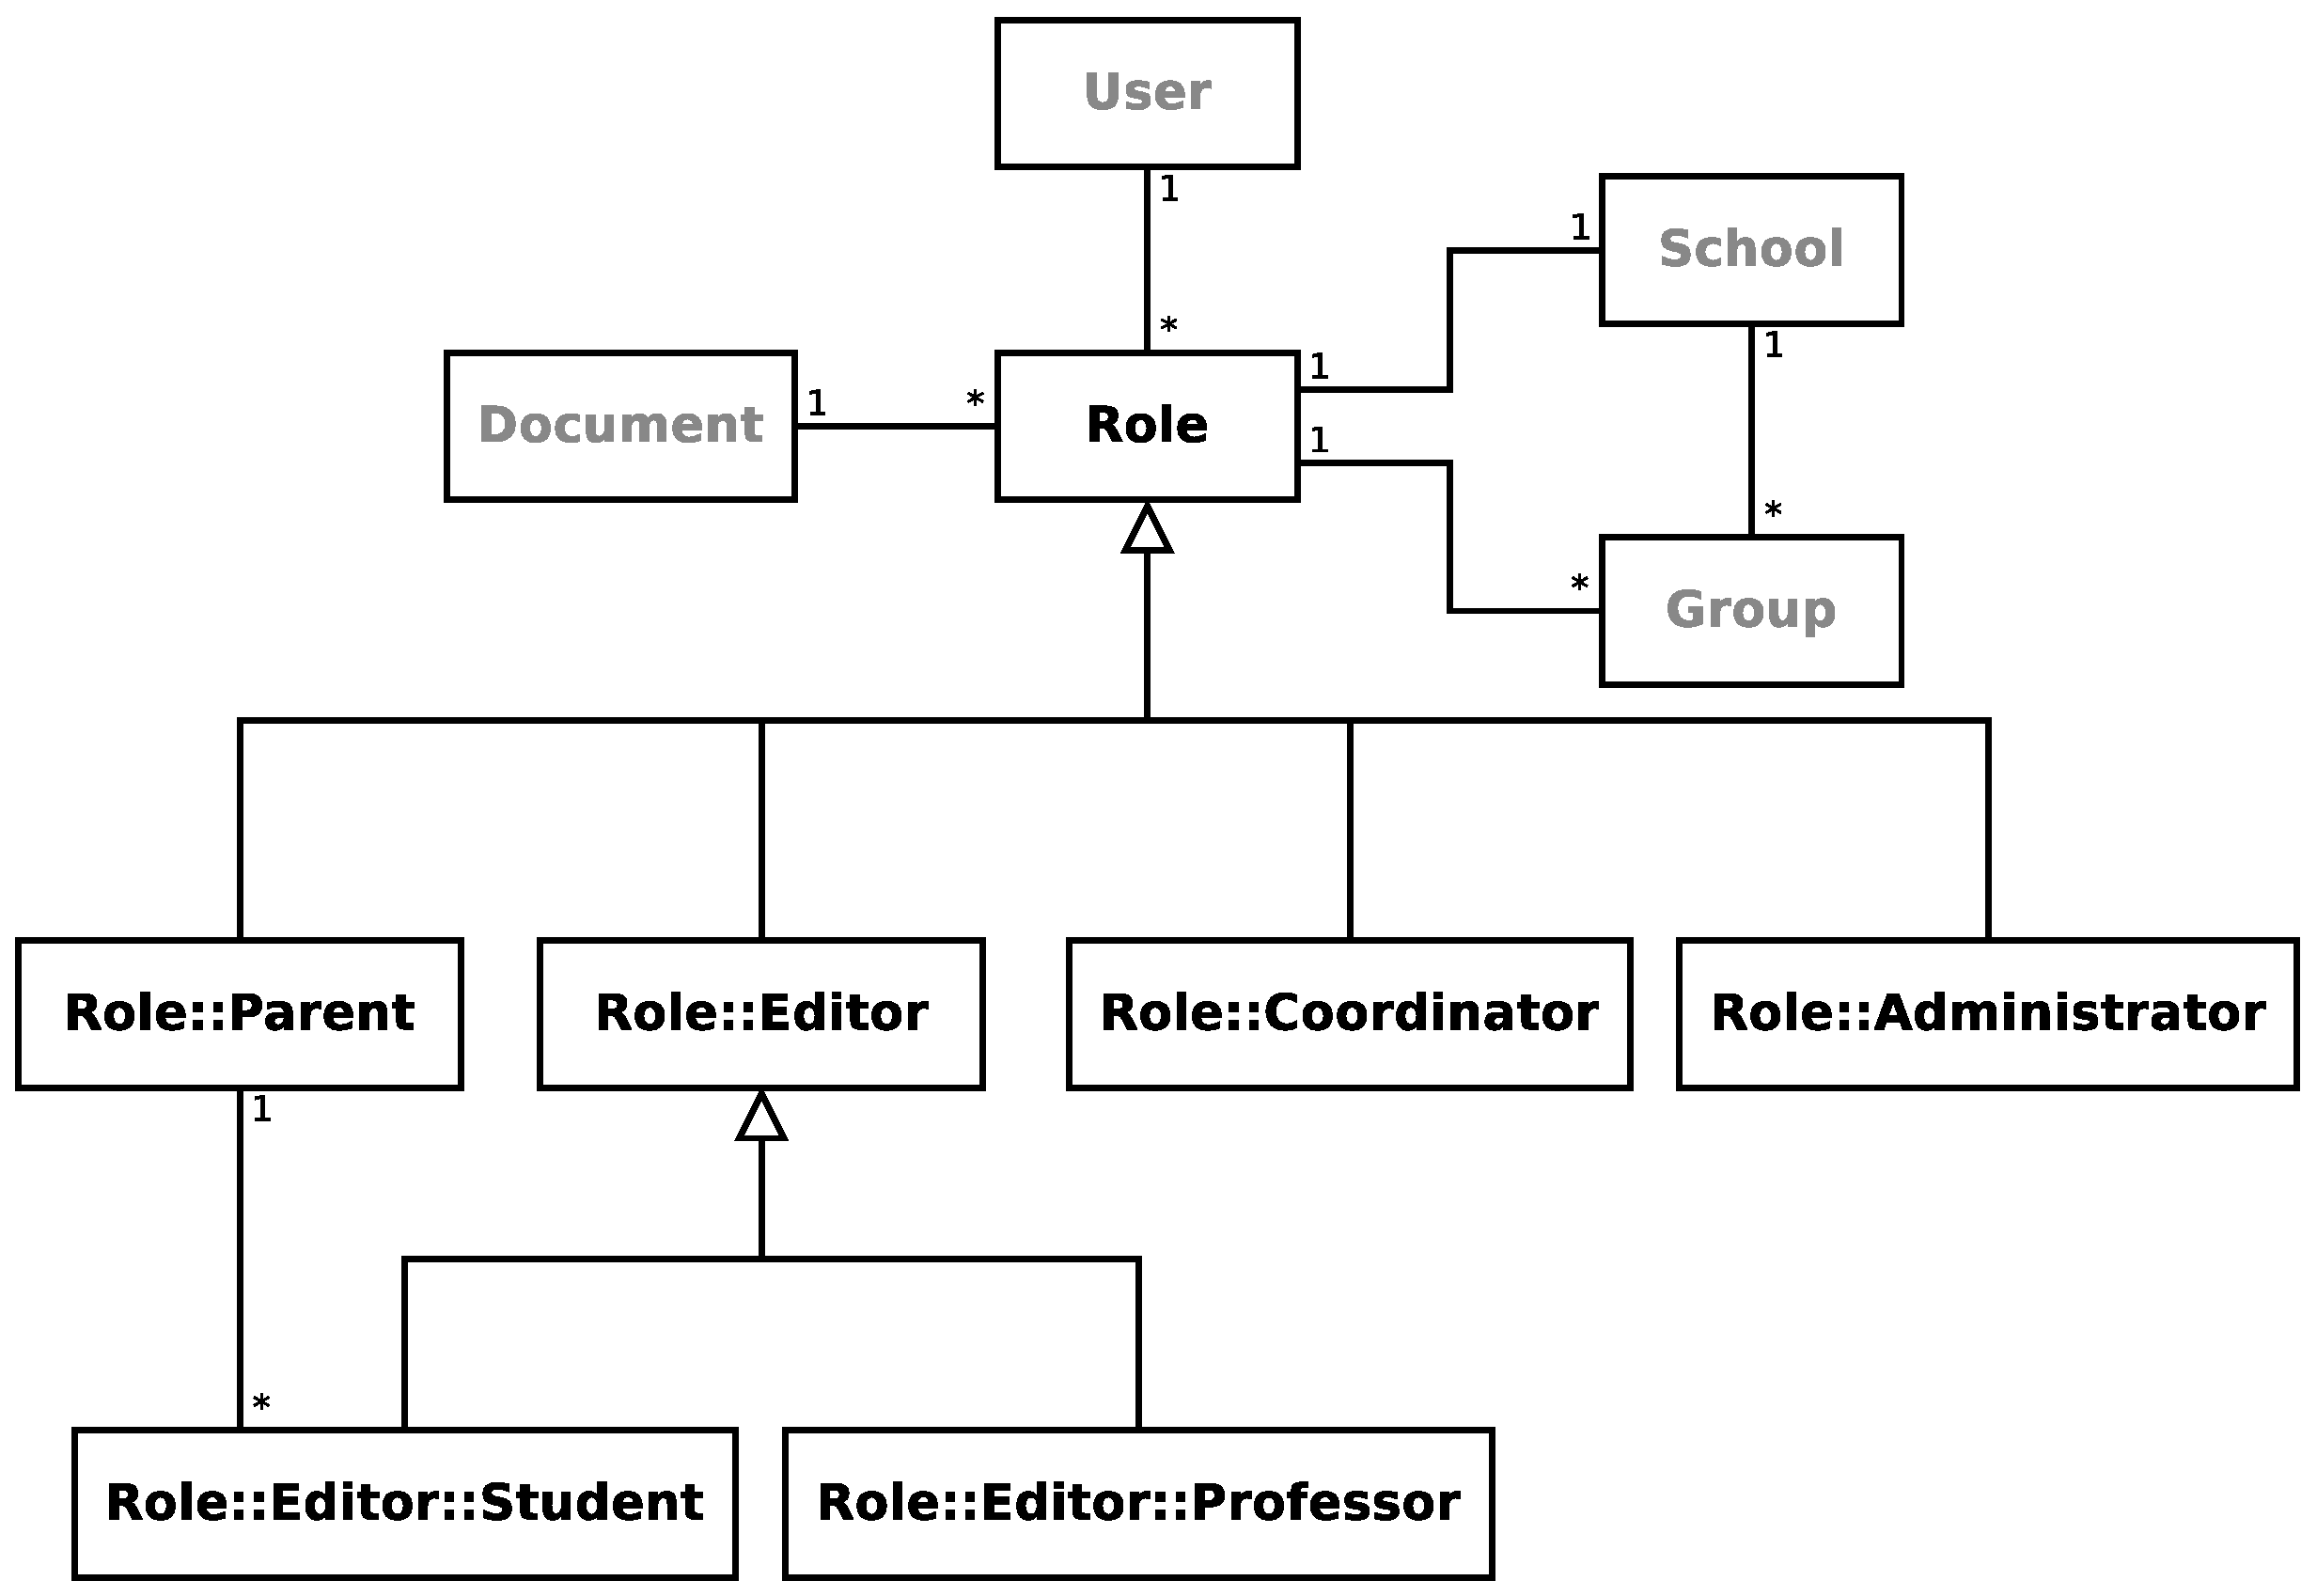
\includegraphics[width=130mm]{user_roles_current}
  \caption{Current User Roles Model}
  \label{fig:user_roles_current}
\end{figure}

\subsubsection{Candidate Patterns}\label{sec:fa_roles_candidate_patterns}

The current logic on roles and users states that a user may be a professor, a student, a parent, a coordinator (in which case it also has a professor role associated), or an administrator. Of these five different types of roles, only two of them are allowed editing privileges, which means that only students and professors have to ability to create and edit documents, which leads to an unnecessary level of complexity. If, for example, it was necessary to have a parent with editing privileges, a new Role, descendant of Role::Editor, would have to be created just for that user.

An obvious solution to this problem would be to tie a ``traditional'' \textsc{Access Control List} (as described in \cite{acls}) to the roles actually in use: this would allow to fine-tune each one of the users permissions and authorization sets while maintaining the codebase clean --- however, the logic surrounding authorization schemas and user roles is built around the \emph{CanCan} Ruby gem \cite{cancan}, which authorizes an user based on his or her roles, while keeping the necessary logic to a minimum.

As such, the usage of a full-fledged ACL is unnecessary. As \emph{CanCan} rules are written in Ruby and are based on the AR engine used by Rails, \emph{CanCan} is capable of handling authorizations based either on Models (MVC) or \emph{instances} of these Models. The application of an ACL to define user permissions would allow a fine-grained control over the actions of every individual --- instances of \emph{User} Model --- on the system. However, the cases when this kind of control is necessary are rare, which would mean that the increase in complexity brought with the usage of an ACL would not be surpassed by its usefulness: it would be necessary to rewrite every rule already defined within \emph{CanCan} and then associate each user on the system with a specific set of rules, instead of maintaining the current setup and writing a few (rare) exceptions for the users the system administrator saw fit.

\subsubsection{Chosen Patterns \& Rationale}\label{sec:fa_roles_chosen_patterns_rationale}

As the implementation of an ACL was discarded in \ref{sec:fa_roles_candidate_patterns}, the best solution is to enhance the already present roles system: a flat Role hierarchy, as described in \cite{baumer_riehle_role_object} would allow for a more flexible authorization scheme, where a User could have one or more roles associated, depending on what actions he would be allowed to do, as shown on Fig.~\ref{fig:user_roles_conceptual}. This also makes the task of creating new roles with different authorization schemes much easier, as there is not a need to conform to any special hierarchy scheme: a new role simply means a new type of user. This clearly contrasts with the previous role's logic, where a multi-level hierarchy was in place.

\begin{figure}[H]
  \centering
  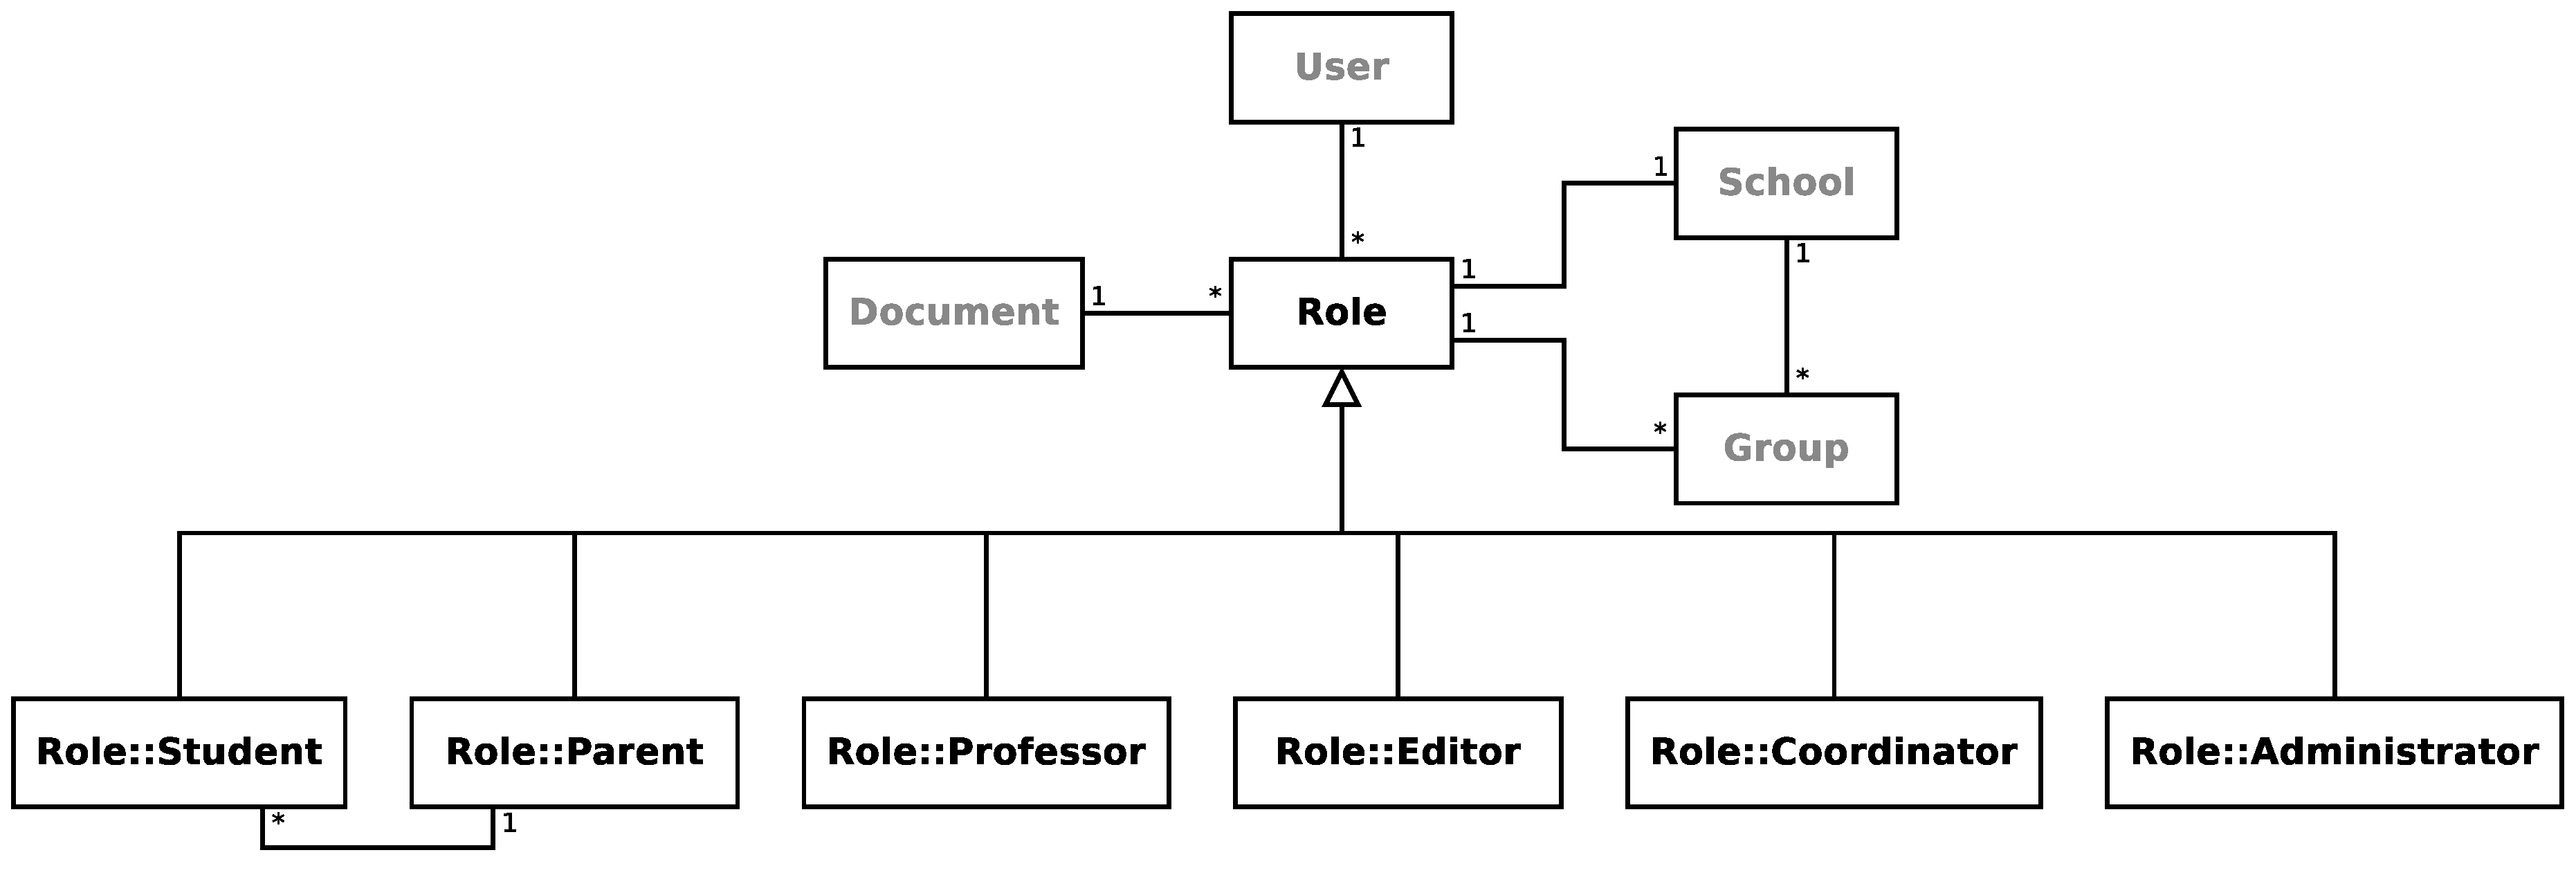
\includegraphics[width=160mm]{user_roles_conceptual}
  \caption{Conceptual User Roles Model}
  \label{fig:user_roles_conceptual}
\end{figure}

\subsubsection{Implementation}\label{sec:fa_roles_implementation}

The refactoring of the roles infrastructure was of very low impact, as codebase and database schema are regarded. The hierarchy of Role classes was flattened, keeping it at only two levels: a generic, non-instantiable class \emph{Role}, and all of its currently existent subclasses: \emph{Editor, Parent, Student, Professor, Coordinator} and \emph{Administrator}. Then, the existent rules were adapted to fit this new hierarchy. The last steps pertains to the modification of the current data to fit the new role organization, which entails analyzing each user current roles and performing the adequate substitutions from the previous roles schema. 

\subsubsection{Impact Analysis}\label{sec:fa_roles_impact_analysis}

The main issues related to the current Roles schema and consequent authorization strategies are caused by the difficulty to capture the constantly evolving necessities of different types of users. As the platform evolves, so do its users and their associated roles. If a new feature is added to the application, it is necessary to define the privileges each user type has over it. The flattening of the Roles hierarchy allows the representation of this Roles as separate, independent objects, allowing the different contexts they refer to be kept separate and also simplify the system configuration.

The usage of a \emph{matricial} ACL implementation, as discussed in \ref{sec:fa_roles_candidate_patterns} would simplify the configuration regarding the privileges of specific users --- allowing a system administrator to have full control over them. Ultimately, this means that the roles would play a very small part in authorization granting, serving only as pre-defined rule sets to be applied to new users.

The usage of a \emph{declarative} ACL (\emph{CanCan}) in conjunction with the \textsc{Role Object} pattern, leads to some important consequences: despite losing the ability to \emph{easily} control the specific set of rules of each user\footnotemark and increasing the difficulty of maintaining constraints between roles, it allows the independent evolution of each \emph{Role}, while making the task of defining their key abstractions regarding each role's position within the platform much more simple and concise.

\footnotetext{This ability  is not completely lost: if necessary, \emph{CanCan} can be used to define authorizations based on a User instance (a specific user)}

%The only relevant point of impact is related to variability. Albeit a low-impact modification, the refactoring of the Roles hierarchy allows for a much quicker role engineering process. This is because a Role now corresponds to a single set of rules, without any hindrance resulting from the previous rule hierarchy. The fact that a multitude of Roles can be associated with a single user allows for a much more wider range of authorizations schemes, as privileges originating from different Roles can be mixed to create unique privilege sets, adapting to a number of different needs.

%\ \\
%\textbf{FIXME: briefly explain how conflicting rules work}





\section{Social Network}\label{sec:fa_social_network}

The current design for the escolinhas.pt social network is dynamic in nature, and extracted from the relationships formed through the connections between users and their roles with schools, groups, and even another roles, as depicted in Fig.~\ref{fig:social_network_current}. This allows the construction of a network where all the connections can be inferred dynamically and where an user can be identified another through their connections: friends, classmates, parent--child, teacher--student, and so on. This network is used mainly in the internal messaging system (and, in a brief future, the instant messaging, or chat system) of \emph{escolinhas.pt}, which allows users to communicate with each other within the platform.

\begin{figure}[H]
  \centering
  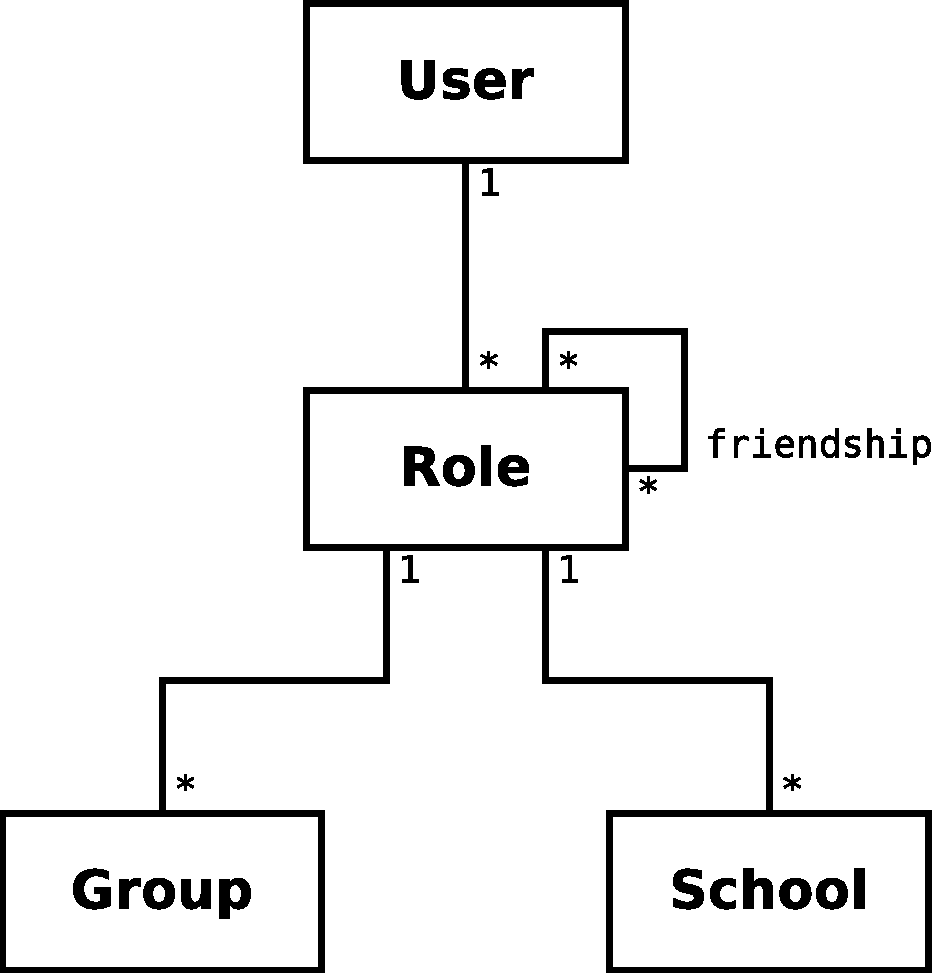
\includegraphics[width=65mm]{social_network_current.pdf}
  \caption{Current User Network Model}
  \label{fig:social_network_current}
\end{figure}

\subsection{Variability Requirements}\label{sec:fa_social_network_variability_requirements}

This model, however useful, offers a very small degree of variability. Due to the closed nature of the platform, there is a need to provide mechanisms able to fine-tune these connections in order to cater to each school specific needs. These mechanisms need to be available at the system administrator level, in order to easily manipulate these links without the need to pollute the application's codebase with hard-coded rules and without the need for redeployement.

\subsection{Candidate Patterns}\label{sec:fa_social_network_candidate_patterns}

Ideally, the user network would be described with a simple, self-referencing model, as shown in figure~\ref{fig:ideal_social_network_users}. This would allow the creation of static relationships between any two users that could be edited as needed. This would work great if all that was needed was to create realtionships between users. However, it is often necessary to create connections between users and other entities in the system, such as groups and schools. Thus, this simple model needs to be abstracted in order to connect any two entities present in the system, whichever they may be, as shown in Fig.~\ref{fig:ideal_social_network_things}.

\begin{figure}[H]
  \centering
  \subfloat[Users Network]{\label{fig:ideal_social_network_users}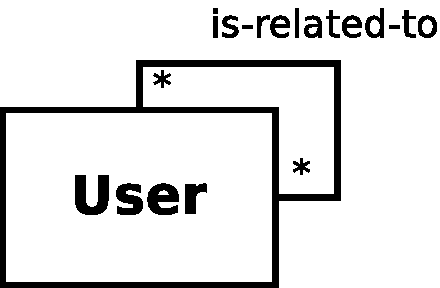
\includegraphics[width=25mm]{ideal_social_network_users}}
  \hspace{20mm}
  \subfloat[Entities Network]{\label{fig:ideal_social_network_things}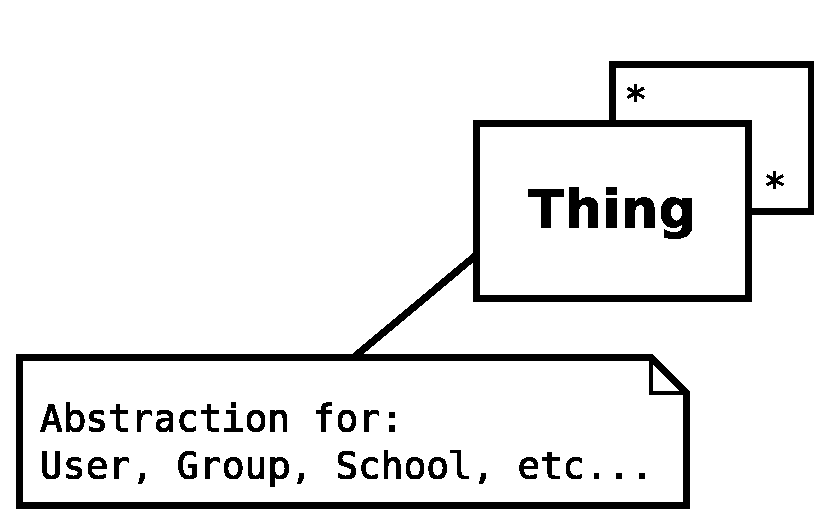
\includegraphics[width=55mm]{ideal_social_network_things}}
  \caption{Simplified Network Models}
  \label{fig:simplified_network_models}
\end{figure}

\subsection{Chosen Patterns \& Rationale}\label{sec:fa_social_network_chosen_patterns_rationale}

Despite solving the majority of the problem, the solutions described in \ref{sec:fa_social_network_candidate_patterns} are less than ideal, as they do not allow the identification of an user before another, because only a direct connection between two different entities is contemplated. As such, for this particular problem, it is necessary to be able to connect any two entities in the system, with an optional third entity to serve as hint as to how the original entities are connected. This problem can be solved by using the \textsc{Accountability} pattern (see \ref{sec:relationships_between_entities}) by Martin Fowler \cite{fowler_accountability}: it allows a bi-directional relationship between two entities (also known as \emph{parties}) while maintaining an AccountabilityType which can be used to store aditional data about the connection. As such, this AccountabilityType can be used to store an optional third party, responsible for identifying how the two other parties are connected --- effectivelly granting means to identify an user before an other, which is part of the original problem formulation (\ref{sec:fa_social_network}).

\subsection{Implementation}\label{sec:fa_social_network_implementation}

A variant of the \textsc{Accountability} design pattern was chosen (shown in Fig.~\ref{fig:social_network_conceptual}). This implementation follows the original description of the pattern by using all the usual entities present in the original \textsc{Accountability} pattern \cite{fowler_accountability} --- however, it denormalizes the AccountabilityType entity \emph{into} the Accountabilities themselves, by placing the AccountabilityType attributes (\verb!type!, \verb!through!, \verb!school_year!, \verb!active!) in the Accountability. Despite creating some data redundancy, this option provides a more performant implementation: as the Accountabilities table is to be constantly accessed, the decision to have the AccountabilityTypes in a separate table would lead to expensive \verb!JOIN! operations. This, in turn, would lead to a less than desirable performance and complexity.

\begin{figure}[H]
  \centering
  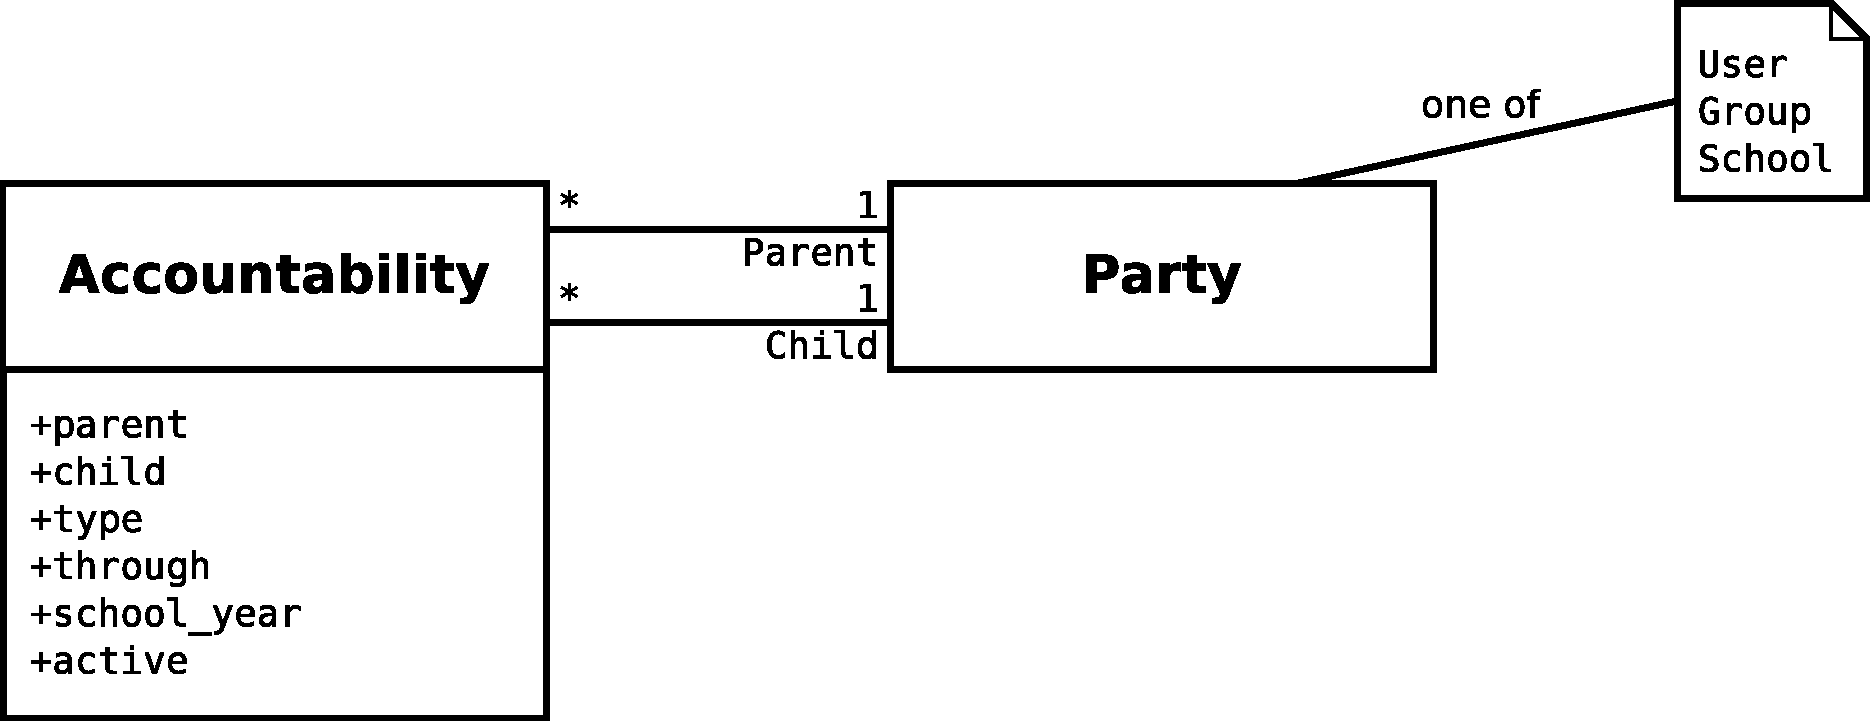
\includegraphics[width=115mm]{social_network_conceptual}
  \caption{Accountability Implementation for User Network}
  \label{fig:social_network_conceptual}
\end{figure}

A series of different AccountabilityTypes were created, in order to cater to a multitude of relationship types:

\begin{itemize}
  \item \textbf{group\_professor:} establishes a connection between a \emph{Group} and a \emph{Professor}, meaning that the user is one of the teacher of \emph{Group}
  \item \textbf{professor:} establishes a connection between two \emph{Users} --- a \emph{Professor} and a \emph{Student} --- creating a teacher-student relationship between them through whichever \emph{Group} they are related to
  \item \textbf{group\_student:} establishes a connection between a \emph{Group} and a \emph{Student}, meaning that the user is part of the \emph{Group} and taught by the \textbf{group\_professors} associated with the aforementioned \emph{Group}
  \item \textbf{school\_professor:} establishes a connection between a \emph{School} and a \emph{Professor}
  \item \textbf{school\_student:} establishes a connection between a \emph{School} and a \emph{Student}
  \item \textbf{parent:} establishes a parenthood relationship between two users
  \item \textbf{school\_coordinator:} dictates an \emph{User} is a coordinator (also known as an administrator) of a certain \emph{School}
  \item \textbf{colleague:} establishes a connection between two \emph{Users} --- either a \emph{Coordinator} or a \emph{Professor} --- through a \emph{School} they both work in
  \item \textbf{student:} establishes a relationship between a \emph{Coordinator} and a \emph{Student} through a \emph{School}
  \item \textbf{school\_parent:} establishes a relationship between a \emph{Coordinator} and a \emph{Parent} through a \emph{School}
  \item \textbf{friend:} establishes a connection between any two \emph{Users} of the system --- whichever their roles may be --- to indicate a friendship relation exists between them
\end{itemize}

% generated with http://truben.no/latex/table/
%\begin{table}
% \begin{tabular}{|l|l|l|l|l|}
%  \hline
%   group\_professor  & Group                 & Professor             & -      & - \\ 
%   professor         & Professor             & Student               & Group  & - \\ 
%   group_student     & Group                 & Student               & -      & - \\ 
%   school\_professor & School                & Professor             & -      & - \\ 
%   school\_student   & School                & Student               & -      & - \\ 
%   parent            & Parent                & Student               & -      & - \\ 
%   school_cordinator & School                & Coordinator           & -      & - \\ 
%   colleague         & Coordinator/Professor & Coordinator/Professor & School & - \\ 
%   student           & Coordinator           & Student               & School & - \\ 
%   school\_parent    & Coordinator           & Parent                & School & - \\ 
%   friend            & User                  & User                  & -      & - \\
%  \hline
% \end{tabular}
%\end{table}

Some of the aforementioned AccountabilityTypes are representative of every type of interpersonal relationship existent in the escolinhas.pt platform. At first sight, some of the AccountabilityTypes created may seem redundant, such as student and school\_parent: they exist because the school coordinator needs to be able to contact everyone who is part of the school. One could argue these connections could easily be inferred through the relations between the coordinator and his or her school, and the relations existent between the school and its students, and finally use the existent parenthood relationships. However, as described in \ref{sec:fa_social_network_variability_requirements}, one of the major design flaws (regarding variability), was the completely dynamic nature of the contacts network. Thus, the choice to implement apparently redundant AccountabilityTypes tied itself with the necessity to have full controll over the existent social relationships. The remainder of the AccountabilityTypes are used to store and facilitate access to membership-like relationships, by stating a certain user is part of a school or group at a given school year. This also allows the platform to keep a history of past (inactive) relationships between entities in the system.

\subsection{Impact Analysis}\label{sec:fa_social_network_impact_analysis}

The usage of this design pattern not only solved some of the existing variability and performance problems, but introduced a new possibility: the ability to create relationships between any two entities in the system. This leads to a very flexible network, capable of being modified at the M0 (data) level (see \ref{sec:aom_architecture}), which is a pre-requisite for end-user level variability.

A second objective pertaining to the application of this pattern was to improve the performance related to contact list creation and the identification of these before the user. This task is currently extremely expensive, with an edge case of 5724 queries needed to fetch and identify 715 contacts. A user with only 18 contacts generates 154 queries. This means that an average of 8 queries are performed for each one of the contacts, meaning the cost of this operation is linear ($O(n)$) in nature, as depicted in Fig.~\ref{fig:queries_per_contacts}. 

The graph in Fig.~\ref{fig:queries_per_contacts} represents the average number of queries performed per number of contacts a user has, and it was sampled from a population of 10000 random users of the platform. One interesting fact arising from this analysis is that the cost growth of the function is not completely linear: due to the dynamic nature of the network, some users may have a sparser network --- e.g. less groups associated with, but more users associated with each group the user is part of --- which can explain the unexpected decrease in the number of queries around the 200-mark and the irregularities in users with less than 100 contacts. However, in practice, this cost is linear enough that one can infer that the number of queries performed is approximately 8 times the number of contacts, which represents a very serious performance issue for one of the most used features of the platform.

%The data used to build the chart can be found in \nameref{sec:appendix_a}

\begin{figure}[H]
  \centering
  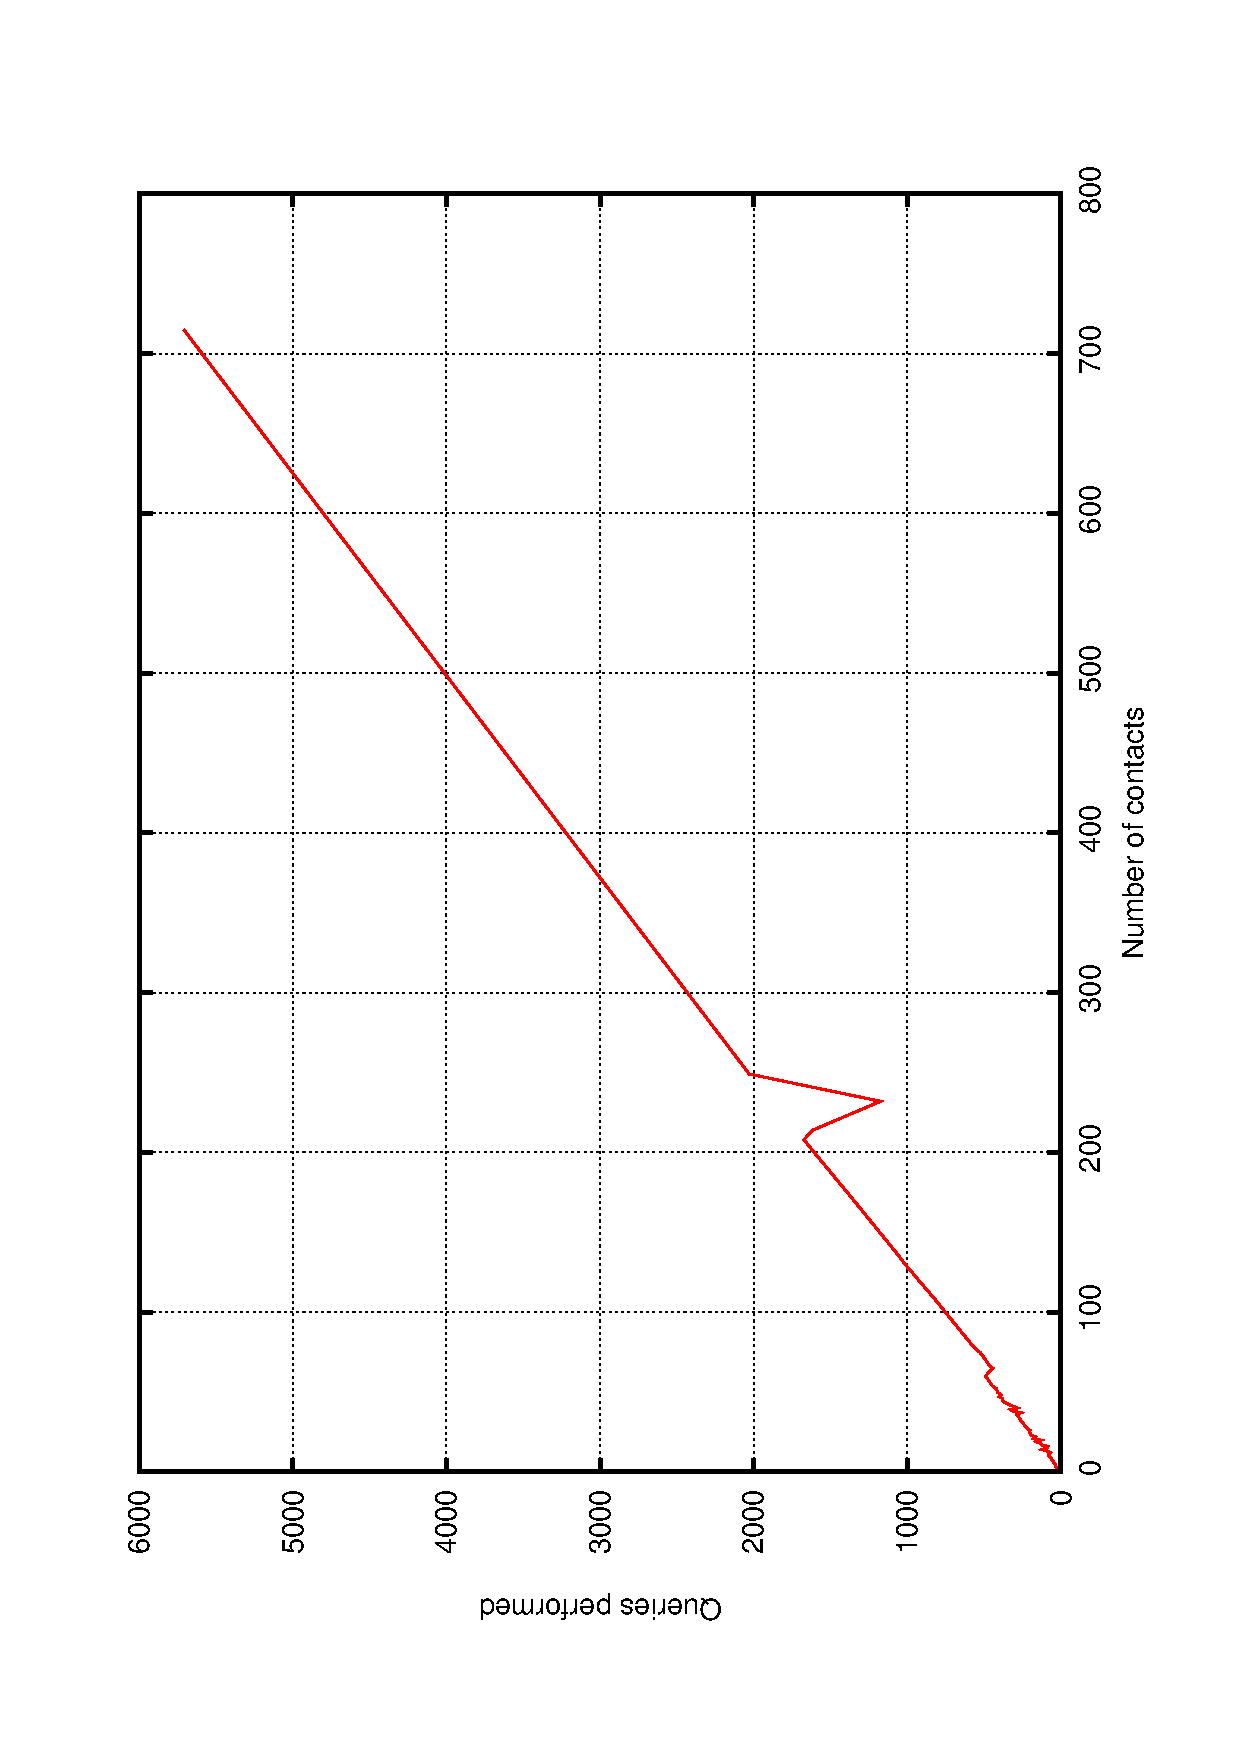
\includegraphics[width=155mm]{queries_per_contacts}
  \caption{Number of queries performed per number of contacts}
  \label{fig:queries_per_contacts}
\end{figure}

The implementation of the \textsc{Accountability} pattern to maintain the relationships between users was able to reduce the cost of the abovementioned task to $O(1)$: only 11 queries are performed to fetch and identify an user contacts, regardless of the size of said contact list. This means that the platform is able to sustain a considerable growth without suffering serious impacts on the performance of seemingly trivial operations.

\ \\
\textbf{NOTE: should Big O notation be used to express operation costs (i.e. number of queries performed)?}








\section{Documents}\label{sec:fa_documents}

\subsection{Variability Requirements}\label{sec:fa_documents_variability_requirements}

The document editor present in \emph{escolinhas.pt} is one of the core components of the system and one of the used features of the platform. This being the case, and due to the constantly evolving nature (\textbf{FIXME: it's not the nature that constantly evolves, but the product}), it is also one of the most modified parts of the system. As it can be seen in Fig.~\ref{fig:documents_current}, this structure has to grow both in size and complexity every time a new type of block content is introduced --- represented by the gray entities in Fig.~\ref{fig:documents_current}. This means that whenever a new type of content is introduced in the system, which happens somewhat frequently --- from three types of blocks (\emph{Paragraphs}, \emph{Drawings} and \emph{ImageDocuments/Photos}) in September 2009 to seven in April/May 2010 --- it is necessary to setup a new \textsc{ActiveRecord} class (along with all the logic for versioning) and a new \textsc{Controller} to accept the requests necessary to create, edit or delete any of these entities. Despite working as intended, this workflow is not adequate to the constant evolution and prototyping the document editor is subjected to.

\begin{figure}[H]
  \centering
  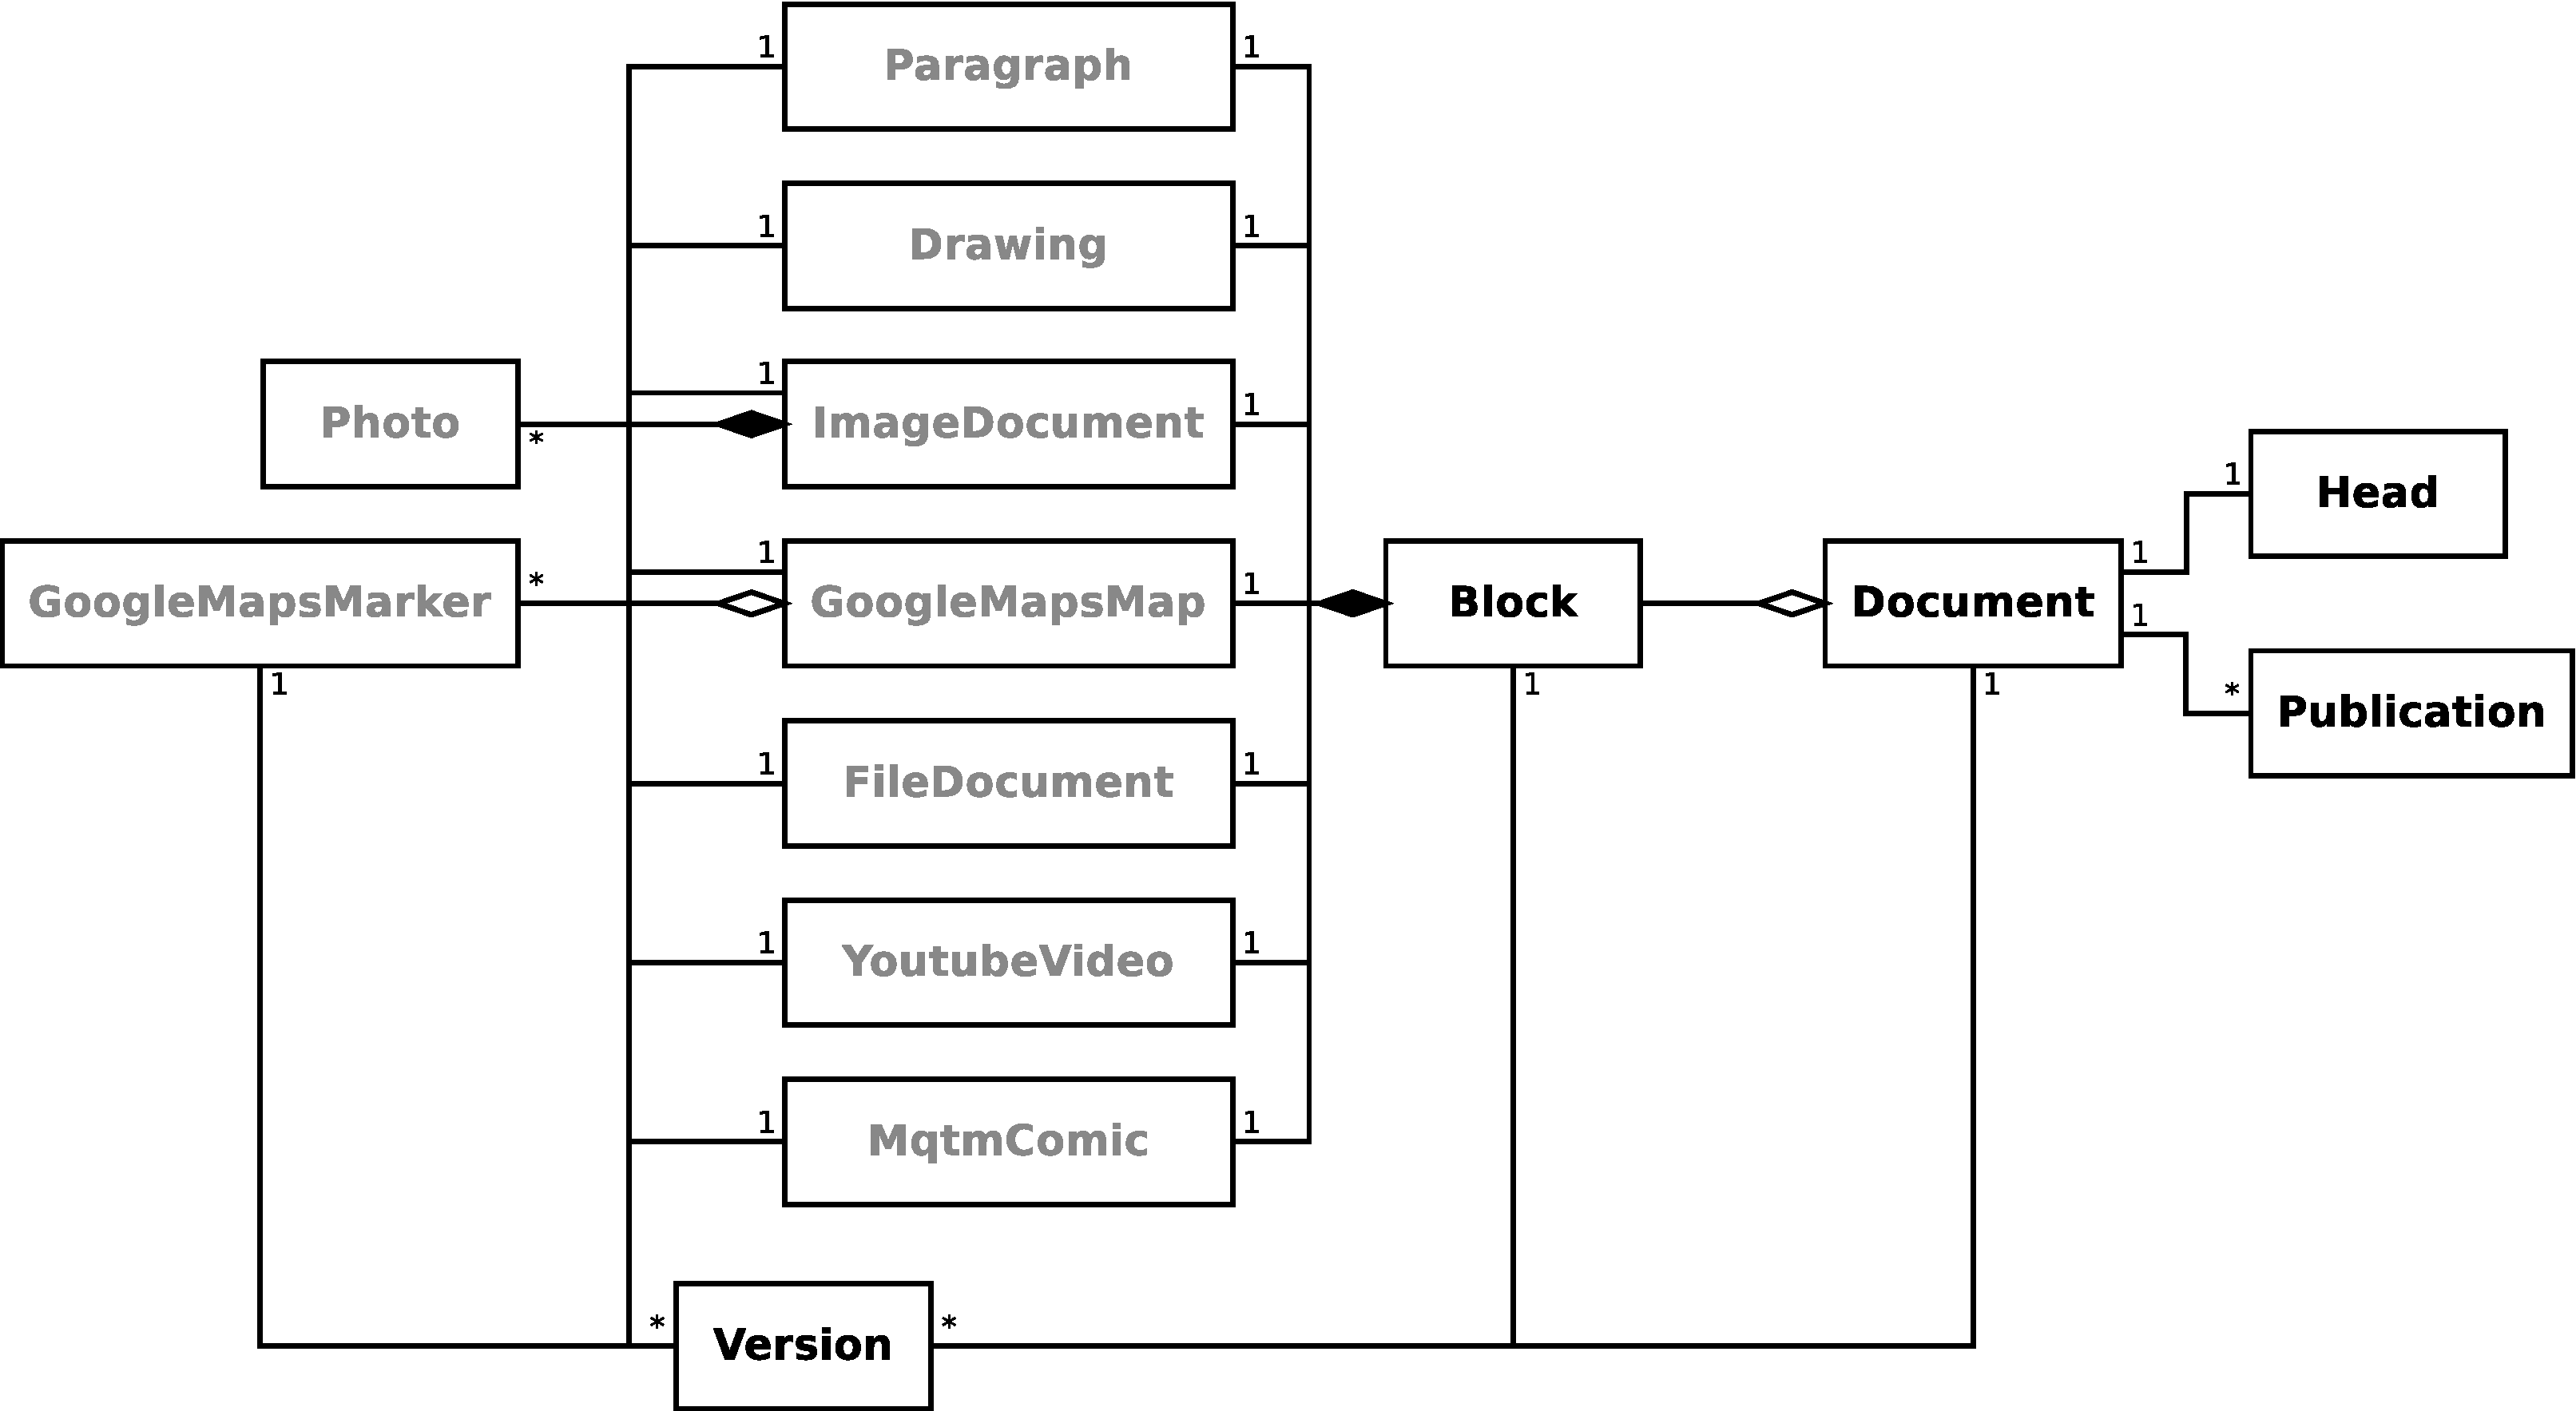
\includegraphics[width=165mm]{documents_current.pdf}
  \caption{Current Documents Model}
  \label{fig:documents_current}
\end{figure}

\subsection{Candidate Patterns}\label{sec:fa_documents_candidate_patterns}

\subsection{Chosen Patterns \& Rationale}\label{sec:fa_documents_chosen_patterns_rationale}

The pattern used is a composite design pattern as described in \cite{riehle_composite_patterns}, where various smaller design patterns work in tandem to create a more complex pattern:

\begin{itemize}
  \item \textsc{Memento} - used for versioning
  \item \textsc{Property} (simplified variant) - used for decoupling a \emph{Block content} from the database schema
  \item \textbf{INVESTIGATE: pattern 3} - the fact that a \emph{Publication} points to a specific \emph{Version} of a \emph{Document} may be a pattern --- it works as a \emph{tag} in a VCS (version control system) system such as git or SVN.
\end{itemize}

\begin{figure}[H]
  \centering
  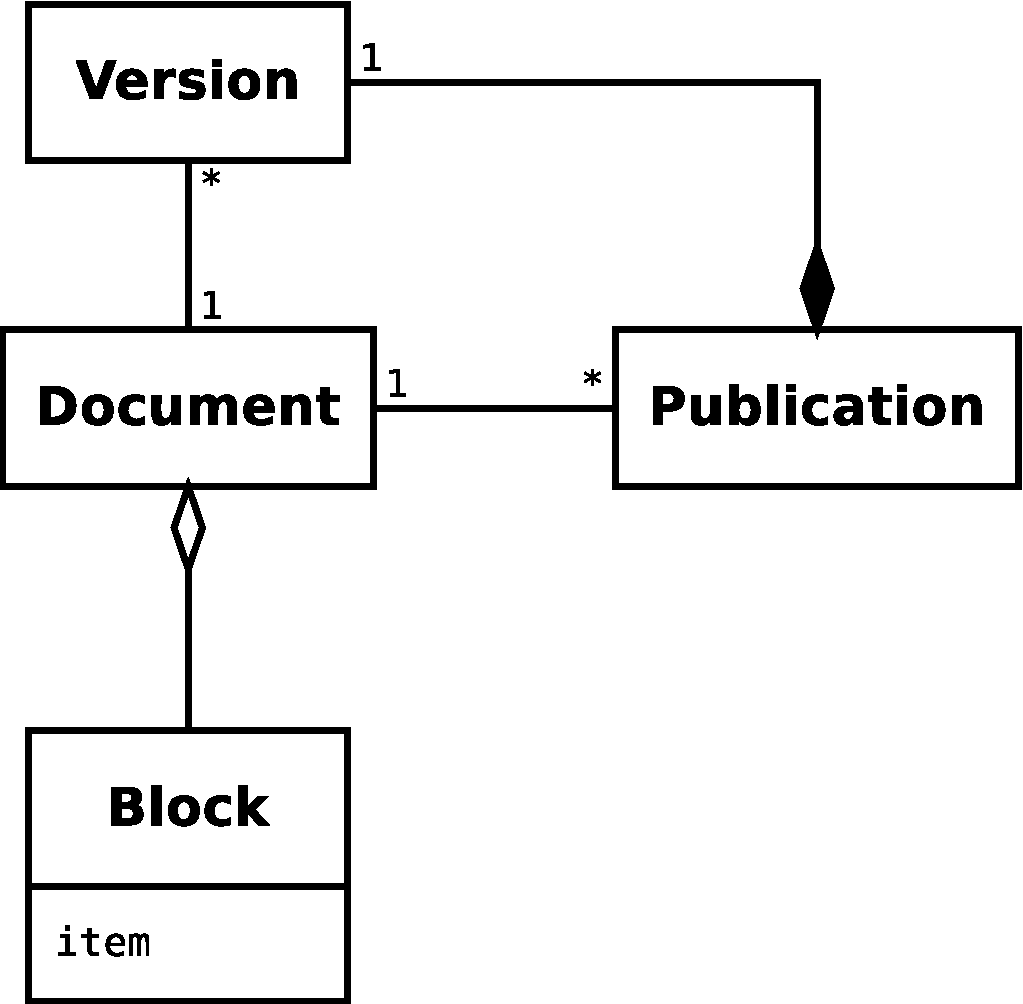
\includegraphics[width=75mm]{documents_conceptual.pdf}
  \caption{Conceptual Documents Model}
  \label{fig:documents_conceptual}
\end{figure}

The variant of the \textsc{Property} pattern implemented is simplified due to the highly dynamic nature of the Ruby language --- which means that, for this particular problem, it is able to build new types of objects or even create new class definitions in runtime, which allows discarding the \textsc{Property}--\textsc{PropertyType} pair (see \ref{sec:property_pattern}) in favour of a single entity, \emph{content}.

\subsection{Implementation}\label{sec:fa_documents_implementation}

The implementation of this composite pattern takes advantage of the highly dynamic nature of the Ruby language and the API provided by the \textsc{ActiveRecord} implementation of Rails.

\emph{Document}, \emph{Block}, \emph{Version} and \emph{Publication} are all AR objects, which means that, according to the AR pattern and the Rails framework conventions, each one of them is stored inside an SQL table, with a row for each one of the attributes. This structure provides the basic blueprint (as stated in \ref{sec:case-study_areas_document_editor}) for the documents to be produced by the editor --- it allows a title, an arbitrary number of orderable blocks, and a snapshot (version) of each modification. It also allows for publications, which essentially point to a specific version of a document.

There is nothing really remarkable about \emph{Blocks}, \emph{Documents} of even \emph{Publications} --- they are ordinary \textsc{ActiveRecord} objects, with associations to each other (as pictured in Fig.~\ref{fig:documents_conceptual}), and explaining how they work is outside of the scope of this study.

However, a \emph{Version} is a bit more complex than a simple AR object, in the sense that it contains a full representation of another AR object at a given point in time --- in this case, a \emph{Document}. This is achieved by serializing a \emph{Document} and all its associations (\emph{Blocks}) in the JSON format, which preserves all the necessary information needed to rebuild a specific \emph{Document} at whichever time that \emph{Version} refers to --- which means that a \emph{Version} effectively implements the \textsc{Memento} design pattern to keep a history of each \emph{Document}.

Finally, a \emph{Block} content possesses special properties that, together with AR, create a dynamic and variable foundation for the development of different types of content. As a \emph{Block} is simply a generic container for an arbitrary type of content, a \emph{Block} content can't be constrained to a single class or object type. The solution is to serialize the content inside the \emph{content} attribute of a \emph{Block}. This way, a \emph{Block} content is simply a string that represents a serialized object --- which can be de-serialized, accessed and modified at runtime. This means that, whichever a \emph{Block} content may be, the content itself is responsible for its representation and life cycle.

In order to further simplify and streamline the development, a \emph{DocumentItem} (super)class was created. This class serves as a staple for further specialization through inheritance, and handles cross-cutting concerns such as object initialization, default values and validations for each of these attribute's values. The need for a specific controller for each one of the different Block items has also been discarded in favour of a single controller, responsible for handling the user input regarding the modification of blocks and their content.

\subsection{Impact Analysis}\label{sec:fa_documents_impact_analysis}

The refactoring of the Document Editor infrastructure had two major points of impact: performance, and variability.


\subsubsection{Performance}

With the current foundation for the editor the number of queries grows linearly with the number of blocks that constitute a document, as it is necessary to perform a query for each one the items related to each one of the blocks. The usage of eager loading is limited due to the polymorphic nature of the blocks and each respective content, which is unknown \emph{a priori}.

From an universe of 3990 documents currently residing in the system (representative of all the documents present in the system as of November 23rd, 2010), the graph present in Fig.~\ref{fig:queries_per_blocks_in_document} shows a linear growth in the number of queries necessary to render a Document: the number of queries necessary are directly proportional to the number of blocks in a document with a 1:1 ratio. Just like in \ref{sec:fa_social_network_impact_analysis}, this represents a serious performance issue: as the most used feature in the \emph{escolinhas.pt} platform, a sustainable growth is very difficult to achieve if the database load increases linearly with the number of existent Documents.

\begin{figure}[H]
  \centering
  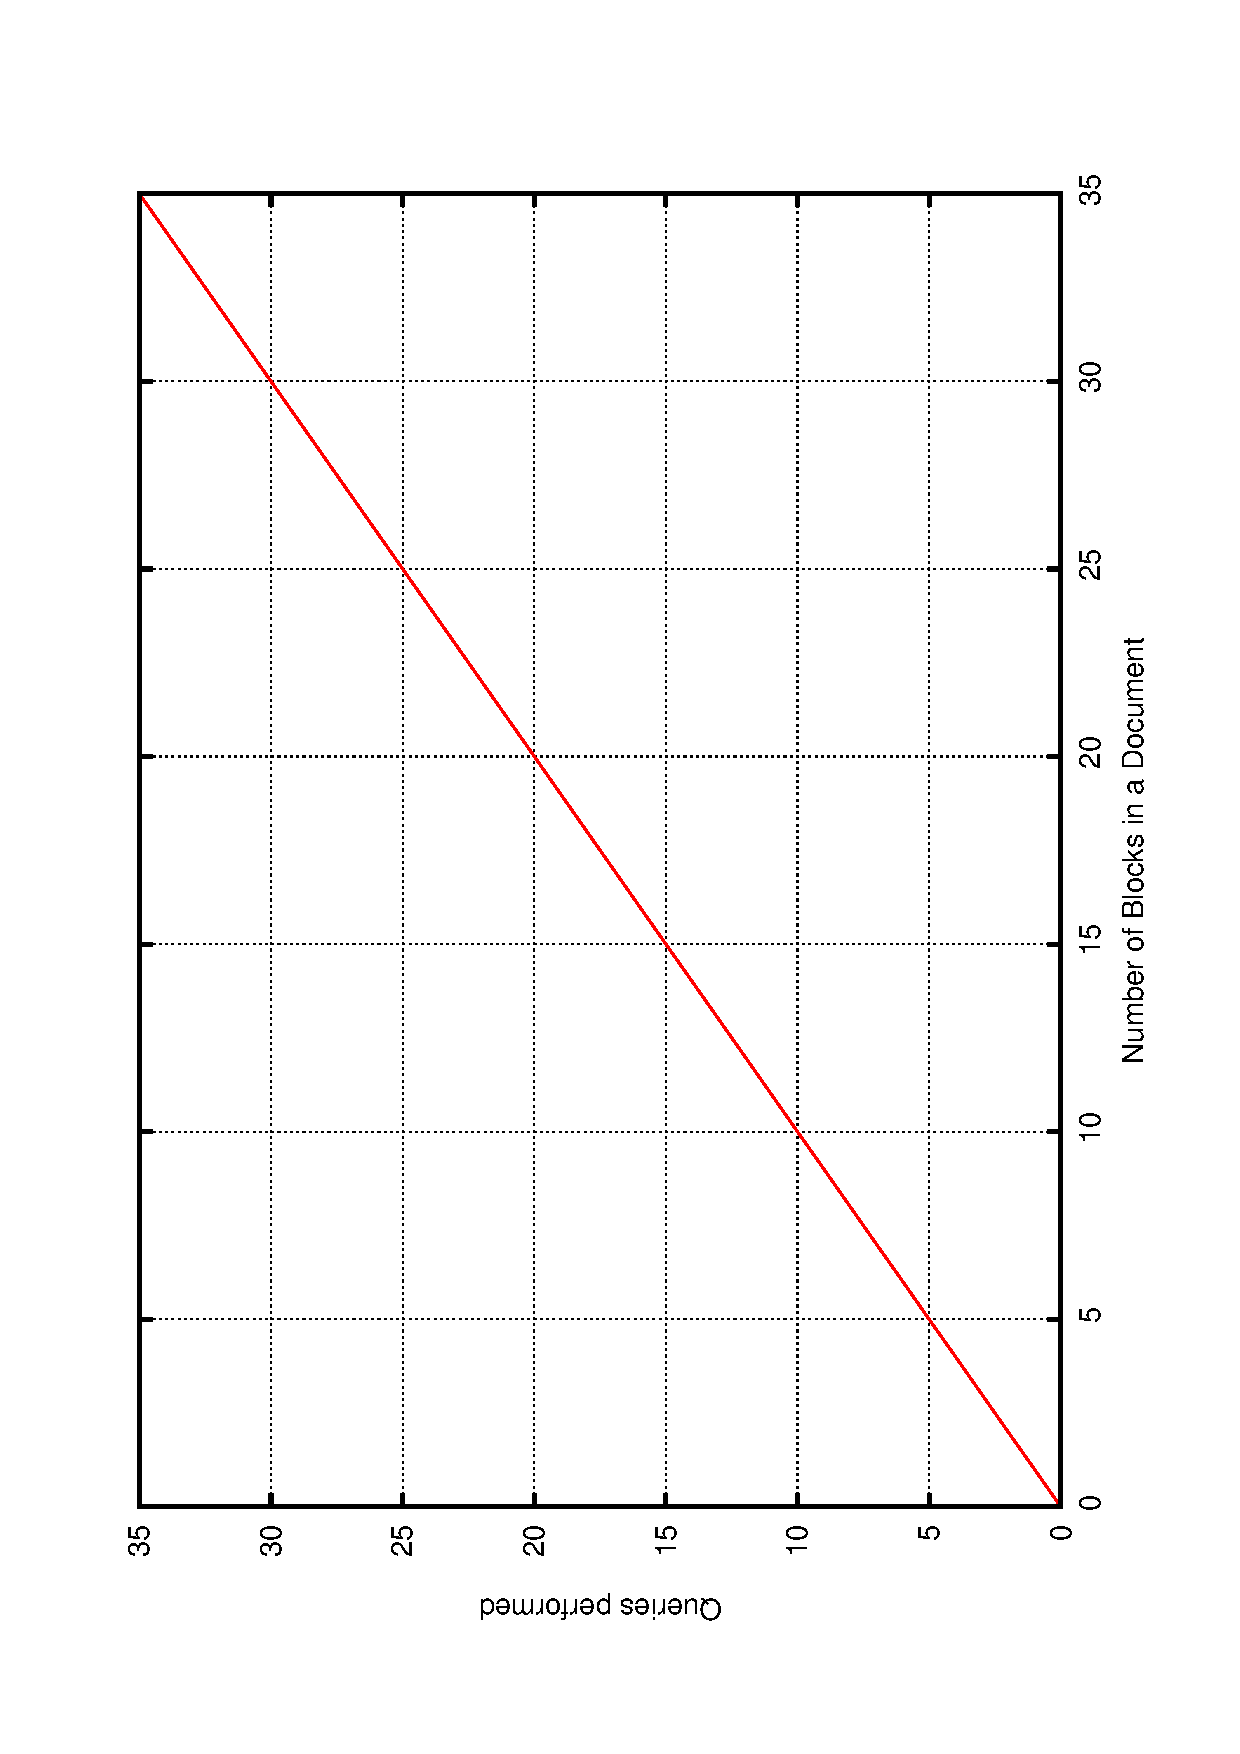
\includegraphics[width=145mm]{document_queries}
  \caption{Number of queries performed per number of Blocks in a single Document}
  \label{fig:queries_per_blocks_in_document}
\end{figure}

The introduction of the model described in \ref{sec:fa_documents_chosen_patterns_rationale} makes the number of queries necessary to display a \emph{Document} to be constant (only 2 queries are performed), as only the Blocks and the Document itself are AR objects --- as the item that constitutes a Block is an integral part of a Block, no queries are necessary to fetch it.

\subsubsection{Variability}

With the introduction of this model, the work necessary to create new types of blocks has been greatly reduced. This allows for much shorter prototyping and testing iteration times --- no database schemas or migrations to worry about, allowing the developers to focus on the details of the model rather than implementation details --- which ultimately leads to a higher degree of variability.











\section{Conclusions}\label{sec:approach_results_conclusions}

This chapter detailed how the study of the current design of the platform was conducted, and the tools used to do so. It described how the data gathered from that study was used to identify what the main problems within the platform were, and how they could be solved. It also described a vast set of applicable design patterns and how this set was reduced to choose the patterns that best solved the problem at hand. Finally, this chapter details the impact regarding the usage of each chosen pattern in terms of variability and performance.




\subsection{User Roles}\label{sec:fa_roles}

Roles play a very important part in any application: by attaching them to users, they allow the application to authenticate and authorize users based on their roles. If an application has a strong tendency to evolve, so do its roles and authorization sets. This section describes the work involved in making the current system of roles used in \emph{escolinhas.pt} as adaptable as possible.

\subsubsection{Variability Requirements}\label{sec:fa_roles_variability_requirements}

Authorization is one of the most sensitive areas of any closed software system: it ensures everyone does only what it should in order to guarantee everything works as expected. In a constantly evolving system, the accesses granted by user roles have a tendency to shift and evolve alongside the application --- either because of new features or a new type of user is required in the system to perform specific tasks. In the context of \emph{escolinhas.pt} this problem ties itself with the ACL used: because of the diversity of roles (Fig.~\ref{fig:user_roles_current}) and the three different usage plans, a lot of different rules are applied to determine if a user can or can not perform certain actions; allied to the growing number of features of the platform, this means that the authorization scheme has to be as flexible as possible to ensure minimal overhead when determining new types of permission sets.

\begin{figure}[h]
  \centering
  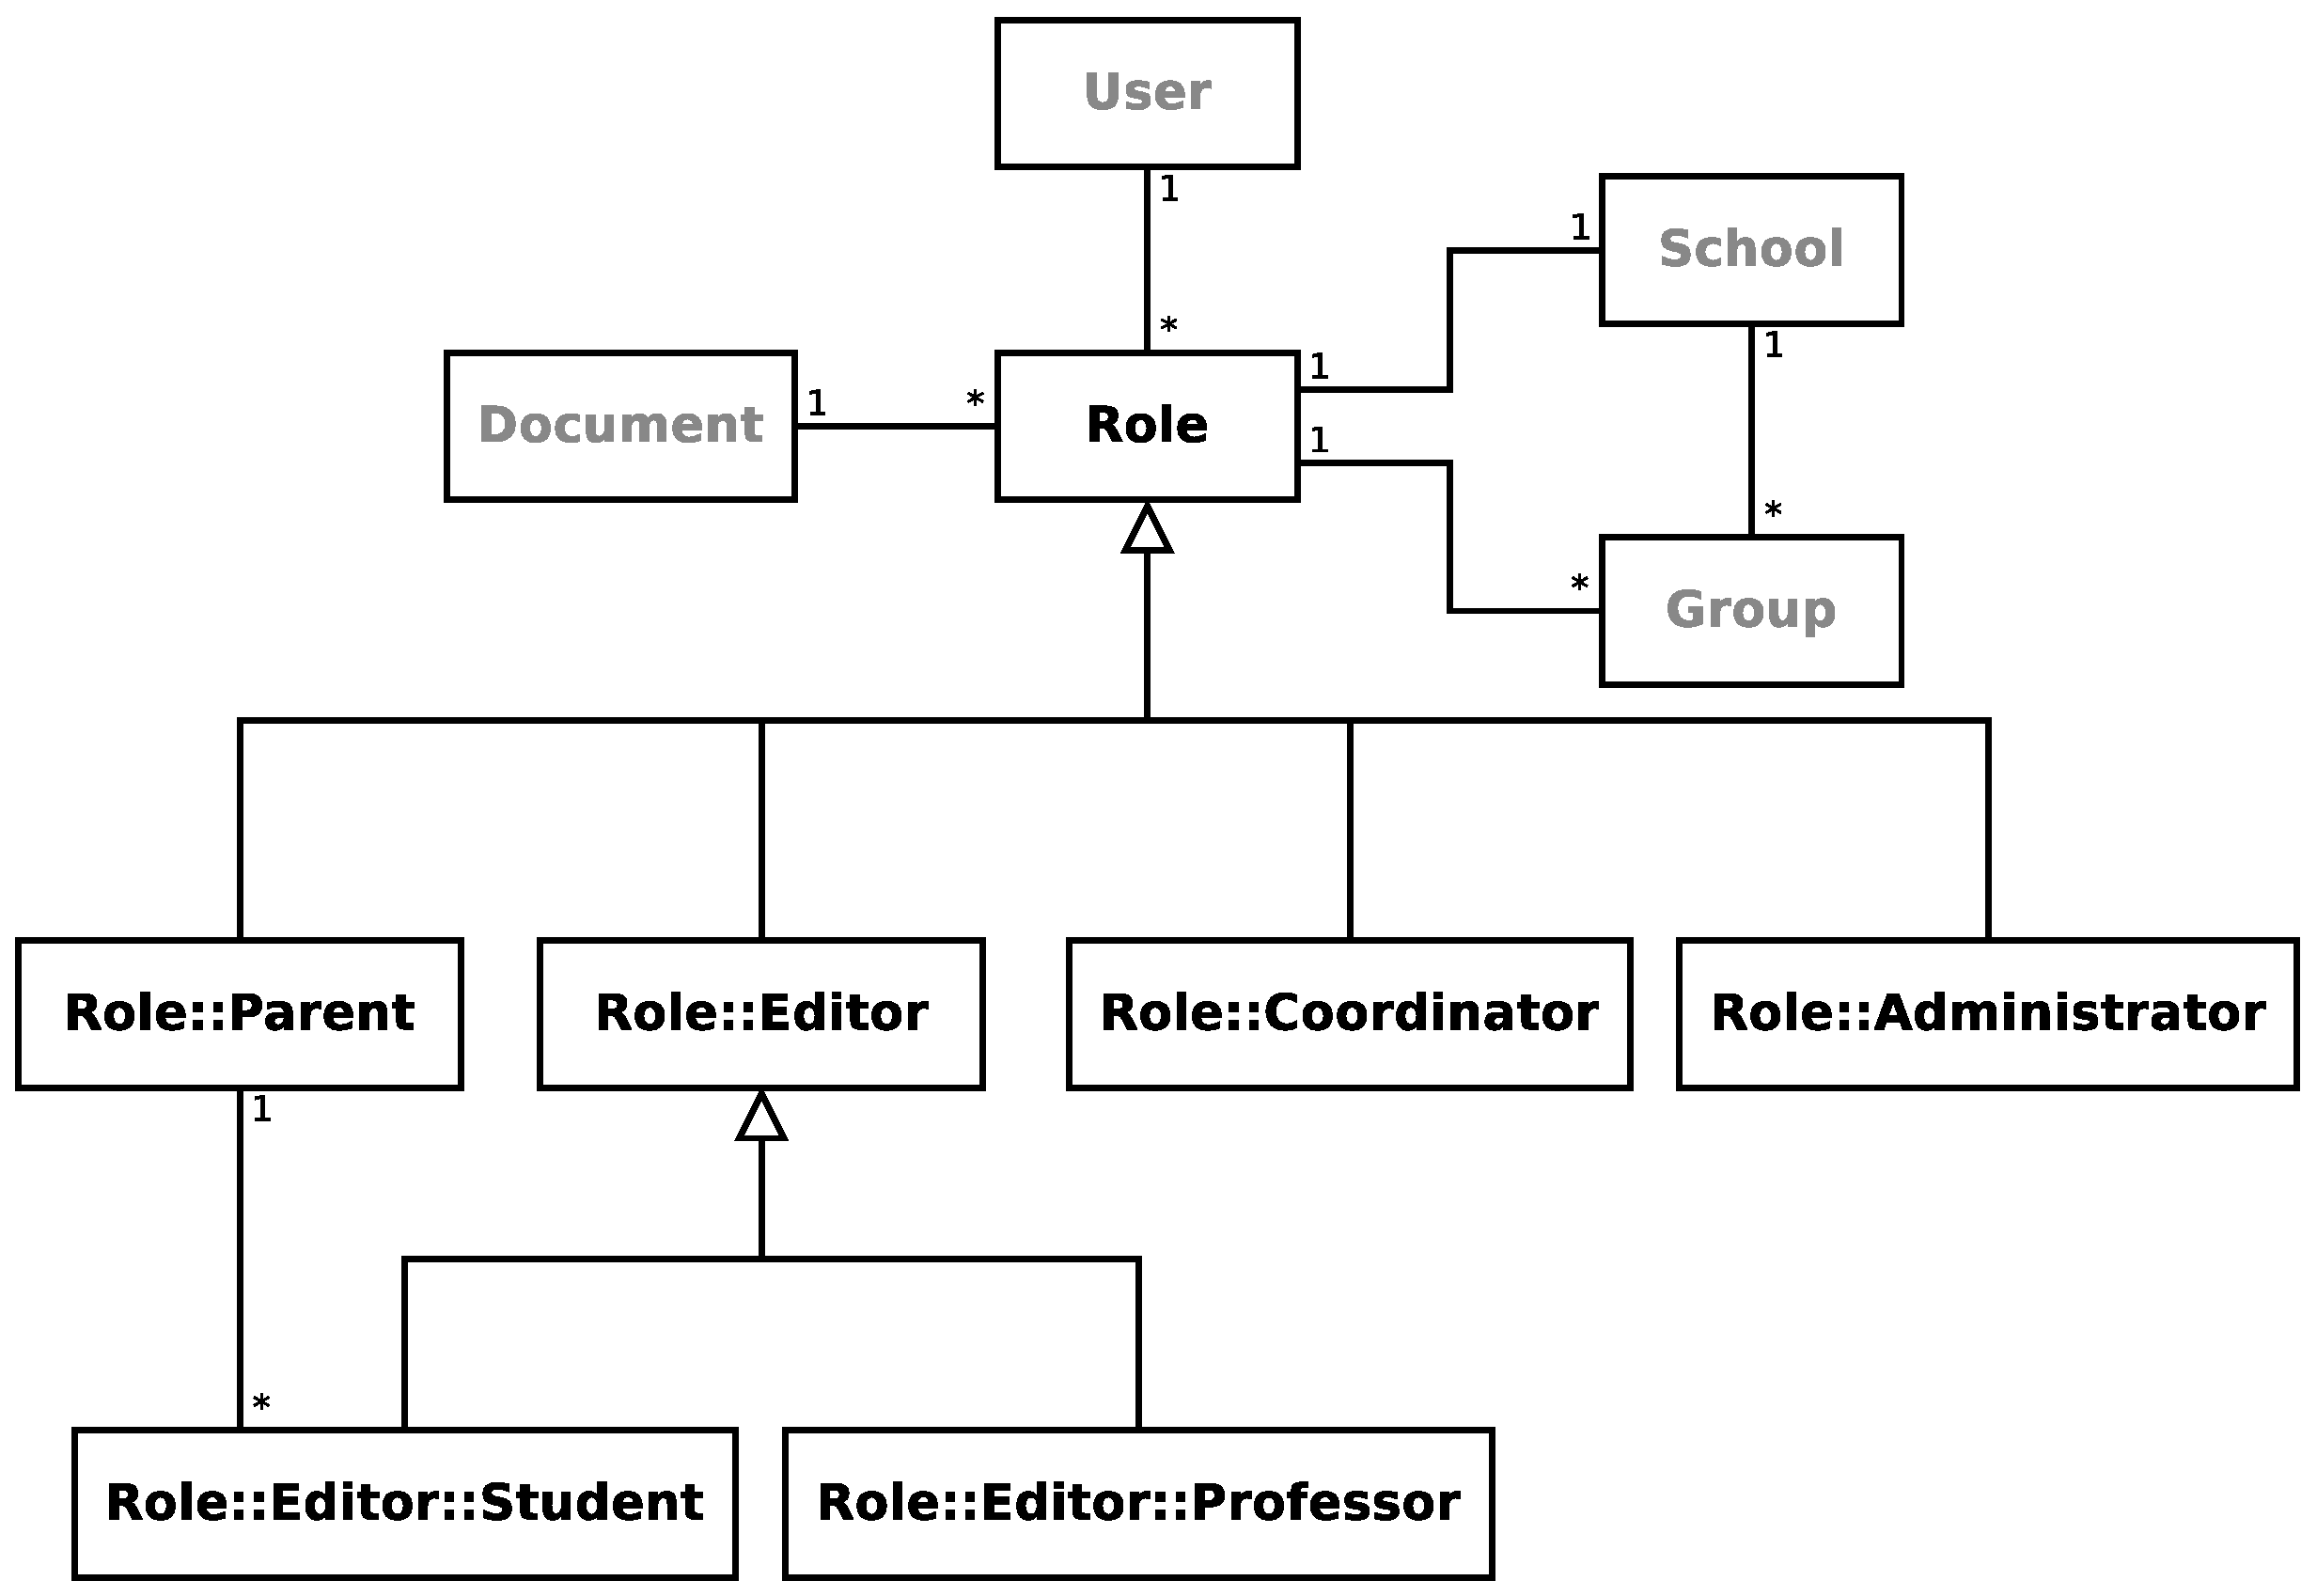
\includegraphics[width=130mm]{user_roles_current}
  \caption{Current User Roles Model}
  \label{fig:user_roles_current}
\end{figure}

\subsubsection{Candidate Patterns}\label{sec:fa_roles_candidate_patterns}

The current logic on roles and users states that a user may be a professor, a student, a parent, a coordinator (in which case it also has a professor role associated), or an administrator. Of these five different types of roles, only two of them are allowed editing privileges, which means that only students and professors have to ability to create and edit documents, which leads to an unnecessary level of complexity. If, for example, it was necessary to have a parent with editing privileges, a new Role, descendant of Role::Editor, would have to be created just for that user.

An obvious solution to this problem would be to tie a ``traditional'' \textsc{Access Control List} (as described in \cite{acls}) to the roles actually in use: this would allow to fine-tune each one of the users permissions and authorization sets while maintaining the codebase clean --- however, the logic surrounding authorization schemas and user roles is built around the \emph{CanCan} Ruby gem \cite{cancan}, which authorizes an user based on his or her roles, while keeping the necessary logic to a minimum.

As such, the usage of a full-fledged ACL is unnecessary. As \emph{CanCan} rules are written in Ruby and are based on the AR engine used by Rails, \emph{CanCan} is capable of handling authorizations based either on Models (MVC) or \emph{instances} of these Models. The application of an ACL to define user permissions would allow a fine-grained control over the actions of every individual --- instances of \emph{User} Model --- on the system. However, the cases when this kind of control is necessary are rare, which would mean that the increase in complexity brought with the usage of an ACL would not be surpassed by its usefulness: it would be necessary to rewrite every rule already defined within \emph{CanCan} and then associate each user on the system with a specific set of rules, instead of maintaining the current setup and writing a few (rare) exceptions for the users the system administrator saw fit.

\subsubsection{Chosen Patterns \& Rationale}\label{sec:fa_roles_chosen_patterns_rationale}

As the implementation of an ACL was discarded in \ref{sec:fa_roles_candidate_patterns}, the best solution is to enhance the already present roles system: a flat Role hierarchy, as described in \cite{baumer_riehle_role_object} would allow for a more flexible authorization scheme, where a User could have one or more roles associated, depending on what actions he would be allowed to do, as shown on Fig.~\ref{fig:user_roles_conceptual}. This also makes the task of creating new roles with different authorization schemes much easier, as there is not a need to conform to any special hierarchy scheme: a new role simply means a new type of user. This clearly contrasts with the previous role's logic, where a multi-level hierarchy was in place.

\begin{figure}[H]
  \centering
  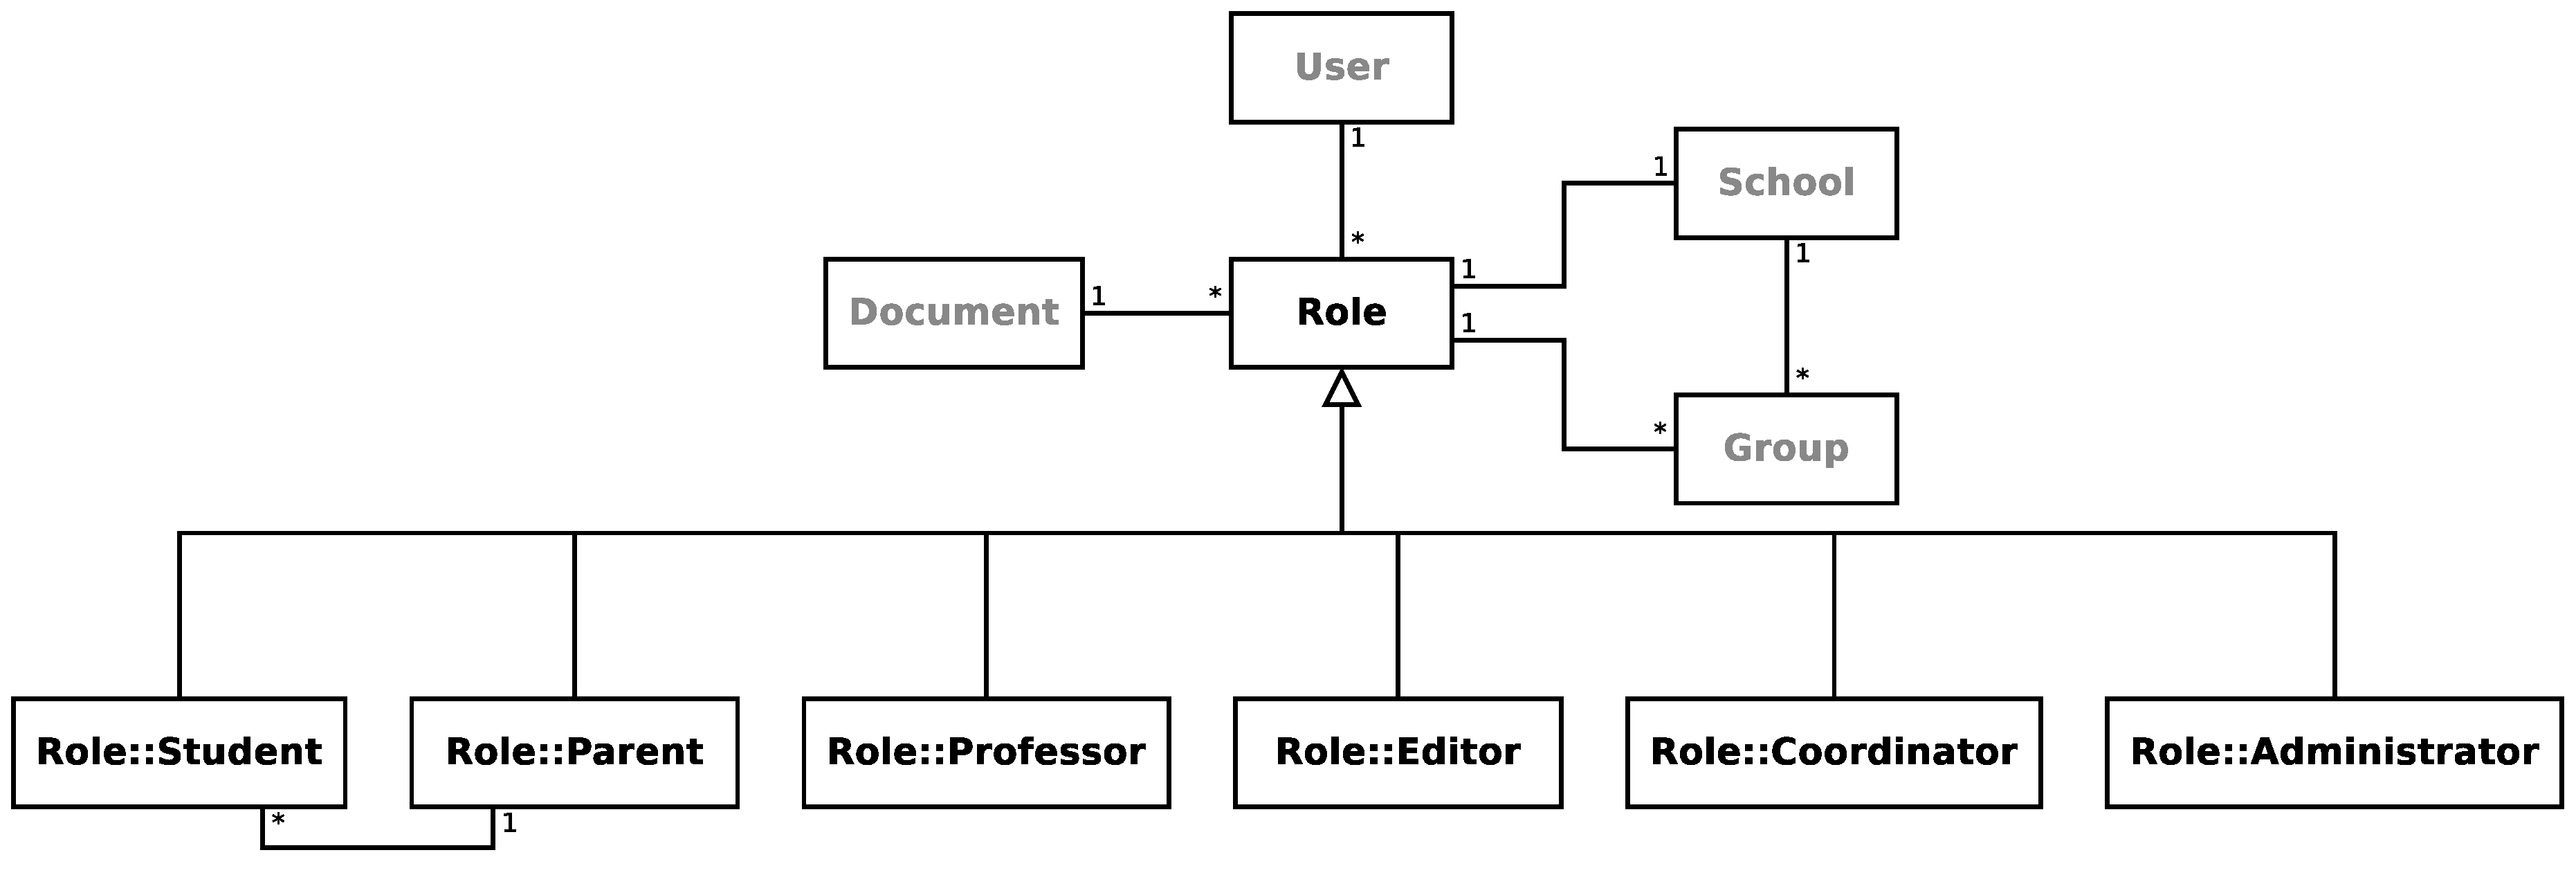
\includegraphics[width=160mm]{user_roles_conceptual}
  \caption{Conceptual User Roles Model}
  \label{fig:user_roles_conceptual}
\end{figure}

\subsubsection{Implementation}\label{sec:fa_roles_implementation}

The refactoring of the roles infrastructure was of very low impact, as codebase and database schema are regarded. The hierarchy of Role classes was flattened, keeping it at only two levels: a generic, non-instantiable class \emph{Role}, and all of its currently existent subclasses: \emph{Editor, Parent, Student, Professor, Coordinator} and \emph{Administrator}. Then, the existent rules were adapted to fit this new hierarchy. The last steps pertains to the modification of the current data to fit the new role organization, which entails analyzing each user current roles and performing the adequate substitutions from the previous roles schema. 

\subsubsection{Impact Analysis}\label{sec:fa_roles_impact_analysis}

The main issues related to the current Roles schema and consequent authorization strategies are caused by the difficulty to capture the constantly evolving necessities of different types of users. As the platform evolves, so do its users and their associated roles. If a new feature is added to the application, it is necessary to define the privileges each user type has over it. The flattening of the Roles hierarchy allows the representation of this Roles as separate, independent objects, allowing the different contexts they refer to be kept separate and also simplify the system configuration.

The usage of a \emph{matricial} ACL implementation, as discussed in \ref{sec:fa_roles_candidate_patterns} would simplify the configuration regarding the privileges of specific users --- allowing a system administrator to have full control over them. Ultimately, this means that the roles would play a very small part in authorization granting, serving only as pre-defined rule sets to be applied to new users.

The usage of a \emph{declarative} ACL (\emph{CanCan}) in conjunction with the \textsc{Role Object} pattern, leads to some important consequences: despite losing the ability to \emph{easily} control the specific set of rules of each user\footnotemark and increasing the difficulty of maintaining constraints between roles, it allows the independent evolution of each \emph{Role}, while making the task of defining their key abstractions regarding each role's position within the platform much more simple and concise.

\footnotetext{This ability  is not completely lost: if necessary, \emph{CanCan} can be used to define authorizations based on a User instance (a specific user)}

%The only relevant point of impact is related to variability. Albeit a low-impact modification, the refactoring of the Roles hierarchy allows for a much quicker role engineering process. This is because a Role now corresponds to a single set of rules, without any hindrance resulting from the previous rule hierarchy. The fact that a multitude of Roles can be associated with a single user allows for a much more wider range of authorizations schemes, as privileges originating from different Roles can be mixed to create unique privilege sets, adapting to a number of different needs.

%\ \\
%\textbf{FIXME: briefly explain how conflicting rules work}





\section{Social Network}\label{sec:fa_social_network}

The current design for the escolinhas.pt social network is dynamic in nature, and extracted from the relationships formed through the connections between users and their roles with schools, groups, and even another roles, as depicted in Fig.~\ref{fig:social_network_current}. This allows the construction of a network where all the connections can be inferred dynamically and where an user can be identified another through their connections: friends, classmates, parent--child, teacher--student, and so on. This network is used mainly in the internal messaging system (and, in a brief future, the instant messaging, or chat system) of \emph{escolinhas.pt}, which allows users to communicate with each other within the platform.

\begin{figure}[H]
  \centering
  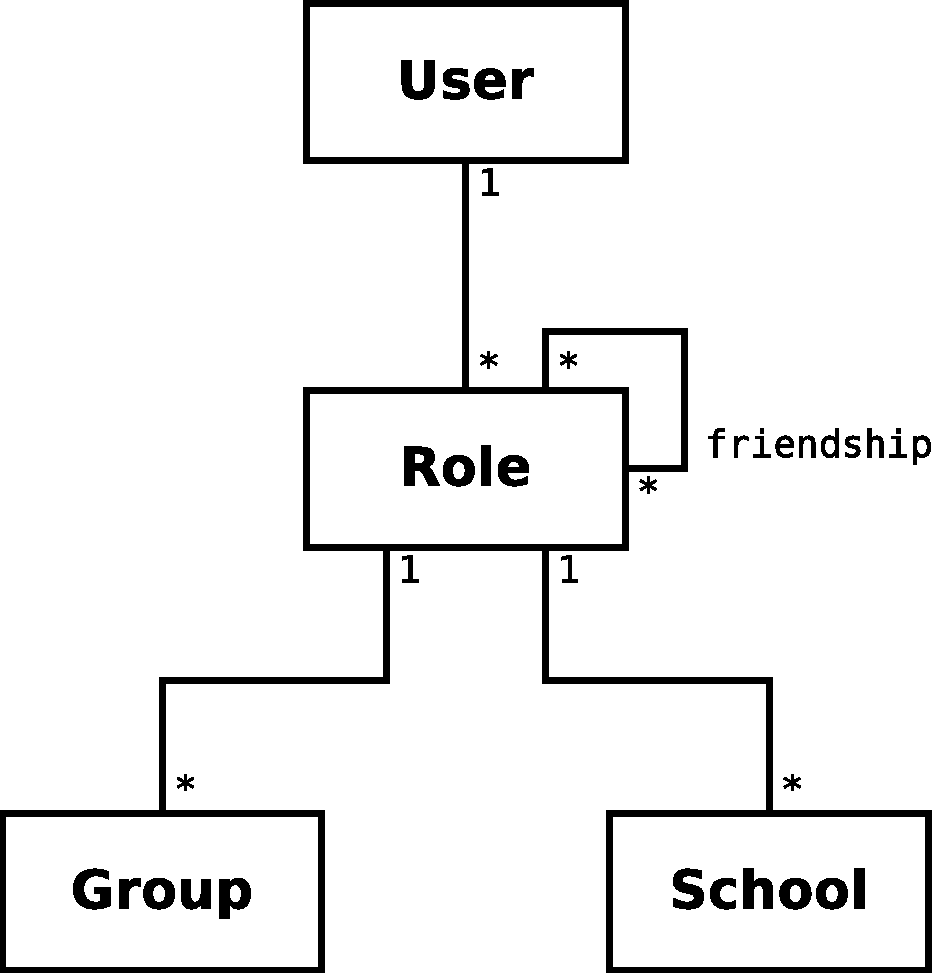
\includegraphics[width=65mm]{social_network_current.pdf}
  \caption{Current User Network Model}
  \label{fig:social_network_current}
\end{figure}

\subsection{Variability Requirements}\label{sec:fa_social_network_variability_requirements}

This model, however useful, offers a very small degree of variability. Due to the closed nature of the platform, there is a need to provide mechanisms able to fine-tune these connections in order to cater to each school specific needs. These mechanisms need to be available at the system administrator level, in order to easily manipulate these links without the need to pollute the application's codebase with hard-coded rules and without the need for redeployement.

\subsection{Candidate Patterns}\label{sec:fa_social_network_candidate_patterns}

Ideally, the user network would be described with a simple, self-referencing model, as shown in figure~\ref{fig:ideal_social_network_users}. This would allow the creation of static relationships between any two users that could be edited as needed. This would work great if all that was needed was to create realtionships between users. However, it is often necessary to create connections between users and other entities in the system, such as groups and schools. Thus, this simple model needs to be abstracted in order to connect any two entities present in the system, whichever they may be, as shown in Fig.~\ref{fig:ideal_social_network_things}.

\begin{figure}[H]
  \centering
  \subfloat[Users Network]{\label{fig:ideal_social_network_users}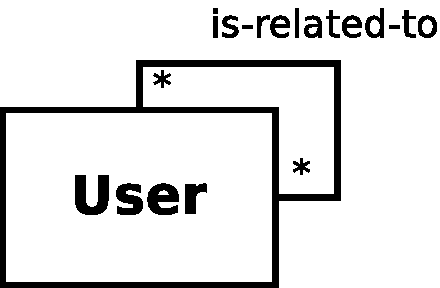
\includegraphics[width=25mm]{ideal_social_network_users}}
  \hspace{20mm}
  \subfloat[Entities Network]{\label{fig:ideal_social_network_things}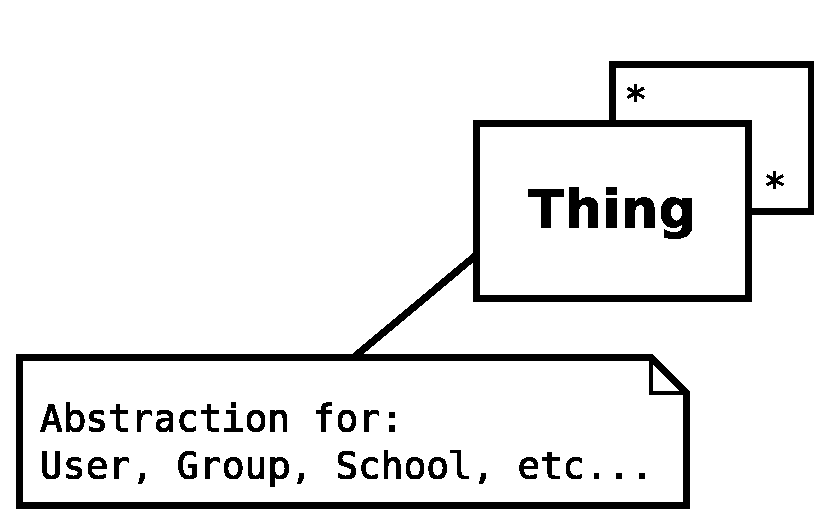
\includegraphics[width=55mm]{ideal_social_network_things}}
  \caption{Simplified Network Models}
  \label{fig:simplified_network_models}
\end{figure}

\subsection{Chosen Patterns \& Rationale}\label{sec:fa_social_network_chosen_patterns_rationale}

Despite solving the majority of the problem, the solutions described in \ref{sec:fa_social_network_candidate_patterns} are less than ideal, as they do not allow the identification of an user before another, because only a direct connection between two different entities is contemplated. As such, for this particular problem, it is necessary to be able to connect any two entities in the system, with an optional third entity to serve as hint as to how the original entities are connected. This problem can be solved by using the \textsc{Accountability} pattern (see \ref{sec:relationships_between_entities}) by Martin Fowler \cite{fowler_accountability}: it allows a bi-directional relationship between two entities (also known as \emph{parties}) while maintaining an AccountabilityType which can be used to store aditional data about the connection. As such, this AccountabilityType can be used to store an optional third party, responsible for identifying how the two other parties are connected --- effectivelly granting means to identify an user before an other, which is part of the original problem formulation (\ref{sec:fa_social_network}).

\subsection{Implementation}\label{sec:fa_social_network_implementation}

A variant of the \textsc{Accountability} design pattern was chosen (shown in Fig.~\ref{fig:social_network_conceptual}). This implementation follows the original description of the pattern by using all the usual entities present in the original \textsc{Accountability} pattern \cite{fowler_accountability} --- however, it denormalizes the AccountabilityType entity \emph{into} the Accountabilities themselves, by placing the AccountabilityType attributes (\verb!type!, \verb!through!, \verb!school_year!, \verb!active!) in the Accountability. Despite creating some data redundancy, this option provides a more performant implementation: as the Accountabilities table is to be constantly accessed, the decision to have the AccountabilityTypes in a separate table would lead to expensive \verb!JOIN! operations. This, in turn, would lead to a less than desirable performance and complexity.

\begin{figure}[H]
  \centering
  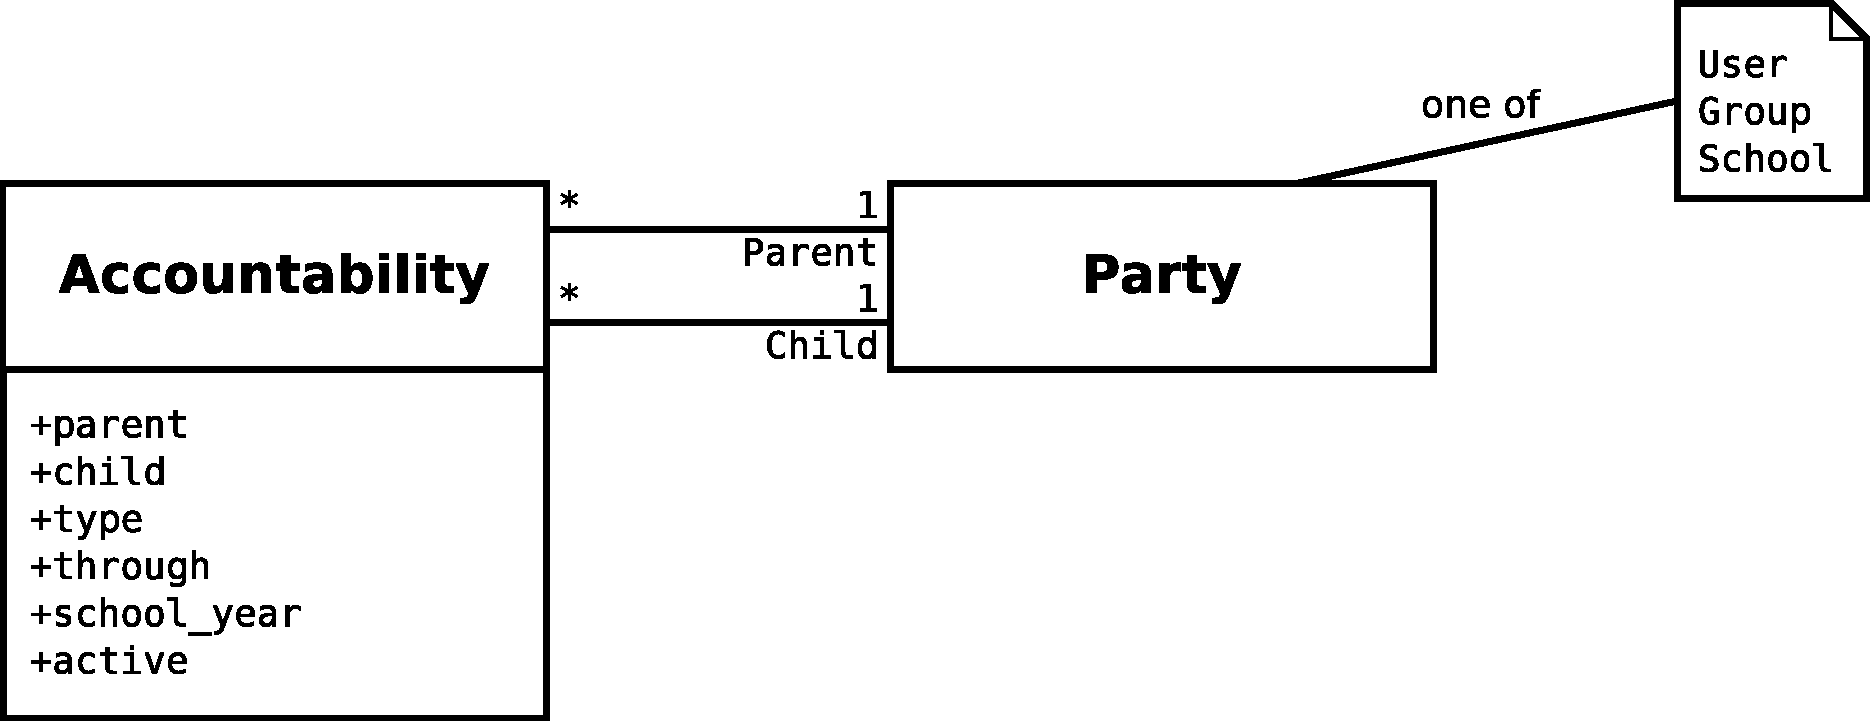
\includegraphics[width=115mm]{social_network_conceptual}
  \caption{Accountability Implementation for User Network}
  \label{fig:social_network_conceptual}
\end{figure}

A series of different AccountabilityTypes were created, in order to cater to a multitude of relationship types:

\begin{itemize}
  \item \textbf{group\_professor:} establishes a connection between a \emph{Group} and a \emph{Professor}, meaning that the user is one of the teacher of \emph{Group}
  \item \textbf{professor:} establishes a connection between two \emph{Users} --- a \emph{Professor} and a \emph{Student} --- creating a teacher-student relationship between them through whichever \emph{Group} they are related to
  \item \textbf{group\_student:} establishes a connection between a \emph{Group} and a \emph{Student}, meaning that the user is part of the \emph{Group} and taught by the \textbf{group\_professors} associated with the aforementioned \emph{Group}
  \item \textbf{school\_professor:} establishes a connection between a \emph{School} and a \emph{Professor}
  \item \textbf{school\_student:} establishes a connection between a \emph{School} and a \emph{Student}
  \item \textbf{parent:} establishes a parenthood relationship between two users
  \item \textbf{school\_coordinator:} dictates an \emph{User} is a coordinator (also known as an administrator) of a certain \emph{School}
  \item \textbf{colleague:} establishes a connection between two \emph{Users} --- either a \emph{Coordinator} or a \emph{Professor} --- through a \emph{School} they both work in
  \item \textbf{student:} establishes a relationship between a \emph{Coordinator} and a \emph{Student} through a \emph{School}
  \item \textbf{school\_parent:} establishes a relationship between a \emph{Coordinator} and a \emph{Parent} through a \emph{School}
  \item \textbf{friend:} establishes a connection between any two \emph{Users} of the system --- whichever their roles may be --- to indicate a friendship relation exists between them
\end{itemize}

% generated with http://truben.no/latex/table/
%\begin{table}
% \begin{tabular}{|l|l|l|l|l|}
%  \hline
%   group\_professor  & Group                 & Professor             & -      & - \\ 
%   professor         & Professor             & Student               & Group  & - \\ 
%   group_student     & Group                 & Student               & -      & - \\ 
%   school\_professor & School                & Professor             & -      & - \\ 
%   school\_student   & School                & Student               & -      & - \\ 
%   parent            & Parent                & Student               & -      & - \\ 
%   school_cordinator & School                & Coordinator           & -      & - \\ 
%   colleague         & Coordinator/Professor & Coordinator/Professor & School & - \\ 
%   student           & Coordinator           & Student               & School & - \\ 
%   school\_parent    & Coordinator           & Parent                & School & - \\ 
%   friend            & User                  & User                  & -      & - \\
%  \hline
% \end{tabular}
%\end{table}

Some of the aforementioned AccountabilityTypes are representative of every type of interpersonal relationship existent in the escolinhas.pt platform. At first sight, some of the AccountabilityTypes created may seem redundant, such as student and school\_parent: they exist because the school coordinator needs to be able to contact everyone who is part of the school. One could argue these connections could easily be inferred through the relations between the coordinator and his or her school, and the relations existent between the school and its students, and finally use the existent parenthood relationships. However, as described in \ref{sec:fa_social_network_variability_requirements}, one of the major design flaws (regarding variability), was the completely dynamic nature of the contacts network. Thus, the choice to implement apparently redundant AccountabilityTypes tied itself with the necessity to have full controll over the existent social relationships. The remainder of the AccountabilityTypes are used to store and facilitate access to membership-like relationships, by stating a certain user is part of a school or group at a given school year. This also allows the platform to keep a history of past (inactive) relationships between entities in the system.

\subsection{Impact Analysis}\label{sec:fa_social_network_impact_analysis}

The usage of this design pattern not only solved some of the existing variability and performance problems, but introduced a new possibility: the ability to create relationships between any two entities in the system. This leads to a very flexible network, capable of being modified at the M0 (data) level (see \ref{sec:aom_architecture}), which is a pre-requisite for end-user level variability.

A second objective pertaining to the application of this pattern was to improve the performance related to contact list creation and the identification of these before the user. This task is currently extremely expensive, with an edge case of 5724 queries needed to fetch and identify 715 contacts. A user with only 18 contacts generates 154 queries. This means that an average of 8 queries are performed for each one of the contacts, meaning the cost of this operation is linear ($O(n)$) in nature, as depicted in Fig.~\ref{fig:queries_per_contacts}. 

The graph in Fig.~\ref{fig:queries_per_contacts} represents the average number of queries performed per number of contacts a user has, and it was sampled from a population of 10000 random users of the platform. One interesting fact arising from this analysis is that the cost growth of the function is not completely linear: due to the dynamic nature of the network, some users may have a sparser network --- e.g. less groups associated with, but more users associated with each group the user is part of --- which can explain the unexpected decrease in the number of queries around the 200-mark and the irregularities in users with less than 100 contacts. However, in practice, this cost is linear enough that one can infer that the number of queries performed is approximately 8 times the number of contacts, which represents a very serious performance issue for one of the most used features of the platform.

%The data used to build the chart can be found in \nameref{sec:appendix_a}

\begin{figure}[H]
  \centering
  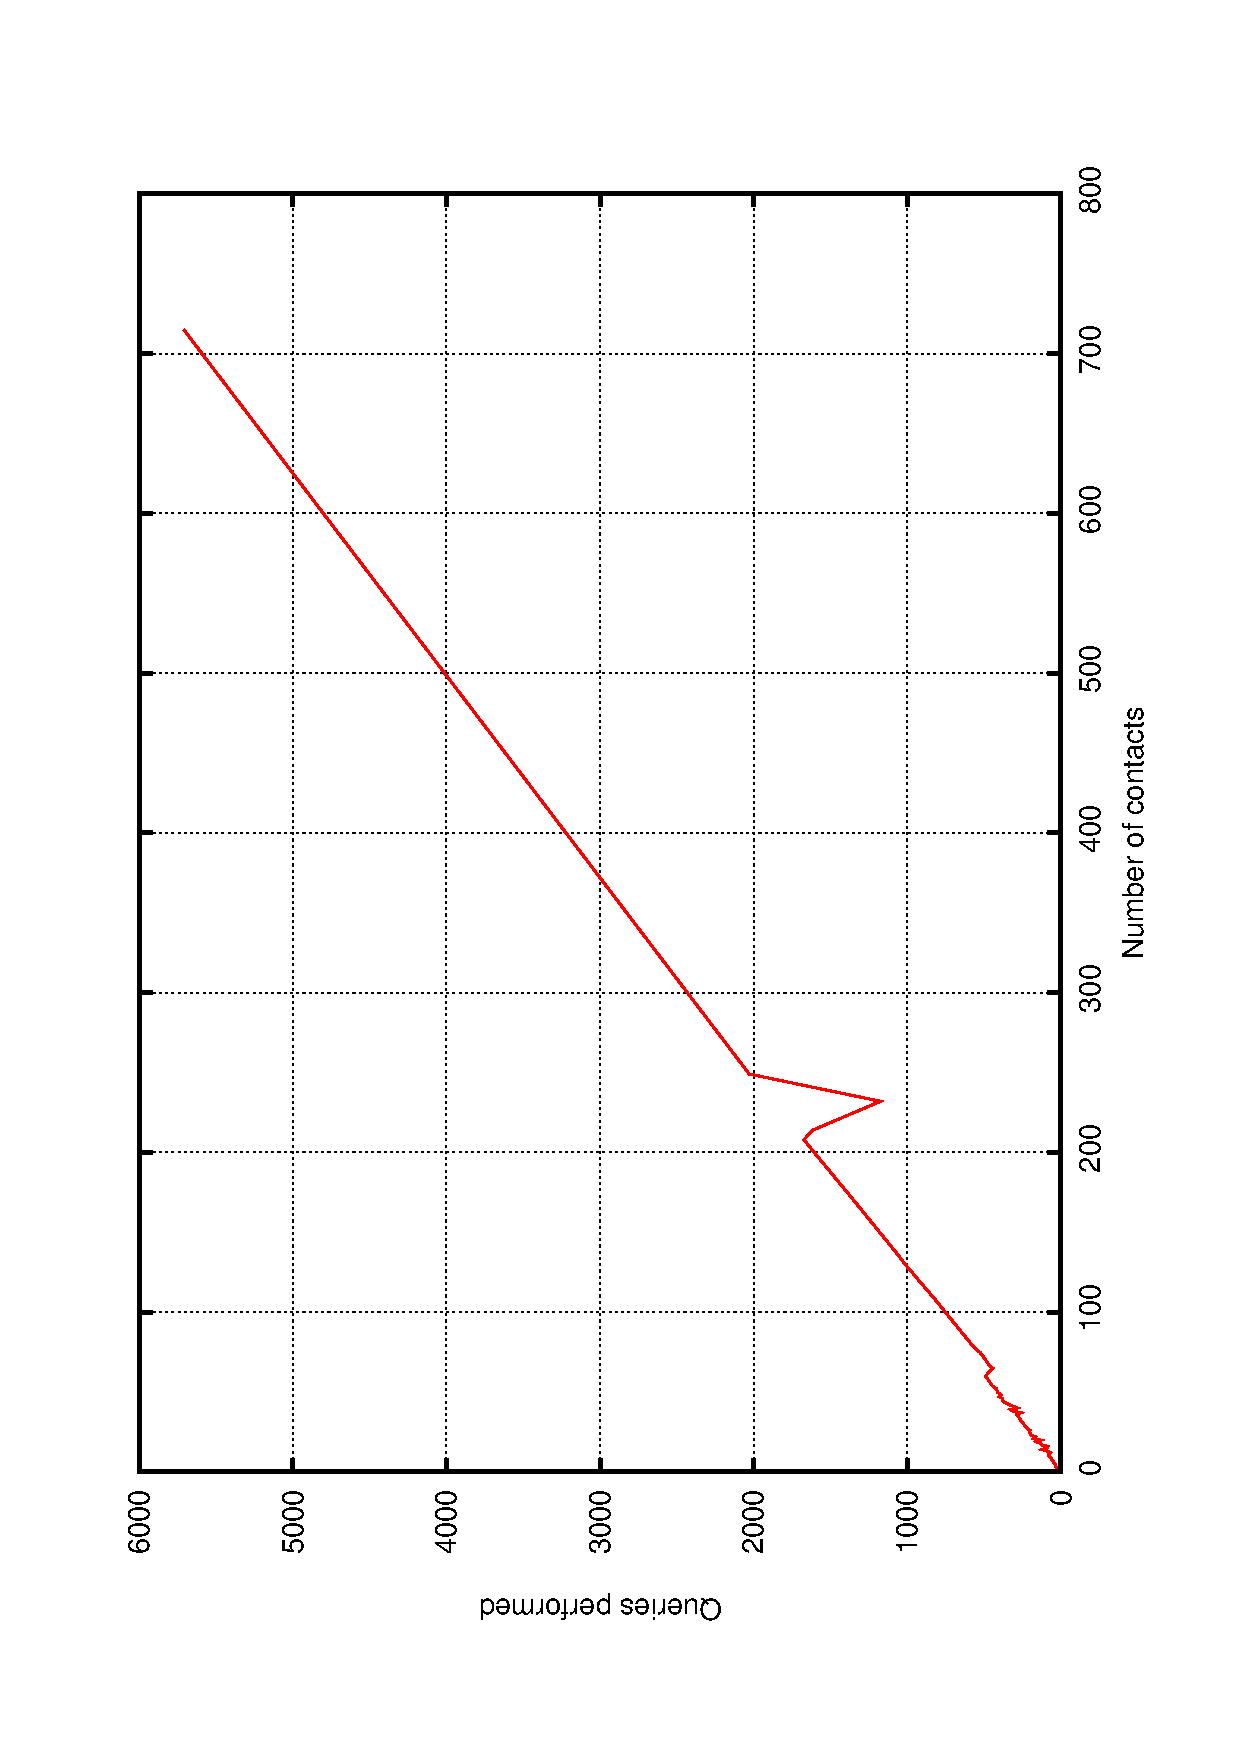
\includegraphics[width=155mm]{queries_per_contacts}
  \caption{Number of queries performed per number of contacts}
  \label{fig:queries_per_contacts}
\end{figure}

The implementation of the \textsc{Accountability} pattern to maintain the relationships between users was able to reduce the cost of the abovementioned task to $O(1)$: only 11 queries are performed to fetch and identify an user contacts, regardless of the size of said contact list. This means that the platform is able to sustain a considerable growth without suffering serious impacts on the performance of seemingly trivial operations.

\ \\
\textbf{NOTE: should Big O notation be used to express operation costs (i.e. number of queries performed)?}








\section{Documents}\label{sec:fa_documents}

\subsection{Variability Requirements}\label{sec:fa_documents_variability_requirements}

The document editor present in \emph{escolinhas.pt} is one of the core components of the system and one of the used features of the platform. This being the case, and due to the constantly evolving nature (\textbf{FIXME: it's not the nature that constantly evolves, but the product}), it is also one of the most modified parts of the system. As it can be seen in Fig.~\ref{fig:documents_current}, this structure has to grow both in size and complexity every time a new type of block content is introduced --- represented by the gray entities in Fig.~\ref{fig:documents_current}. This means that whenever a new type of content is introduced in the system, which happens somewhat frequently --- from three types of blocks (\emph{Paragraphs}, \emph{Drawings} and \emph{ImageDocuments/Photos}) in September 2009 to seven in April/May 2010 --- it is necessary to setup a new \textsc{ActiveRecord} class (along with all the logic for versioning) and a new \textsc{Controller} to accept the requests necessary to create, edit or delete any of these entities. Despite working as intended, this workflow is not adequate to the constant evolution and prototyping the document editor is subjected to.

\begin{figure}[H]
  \centering
  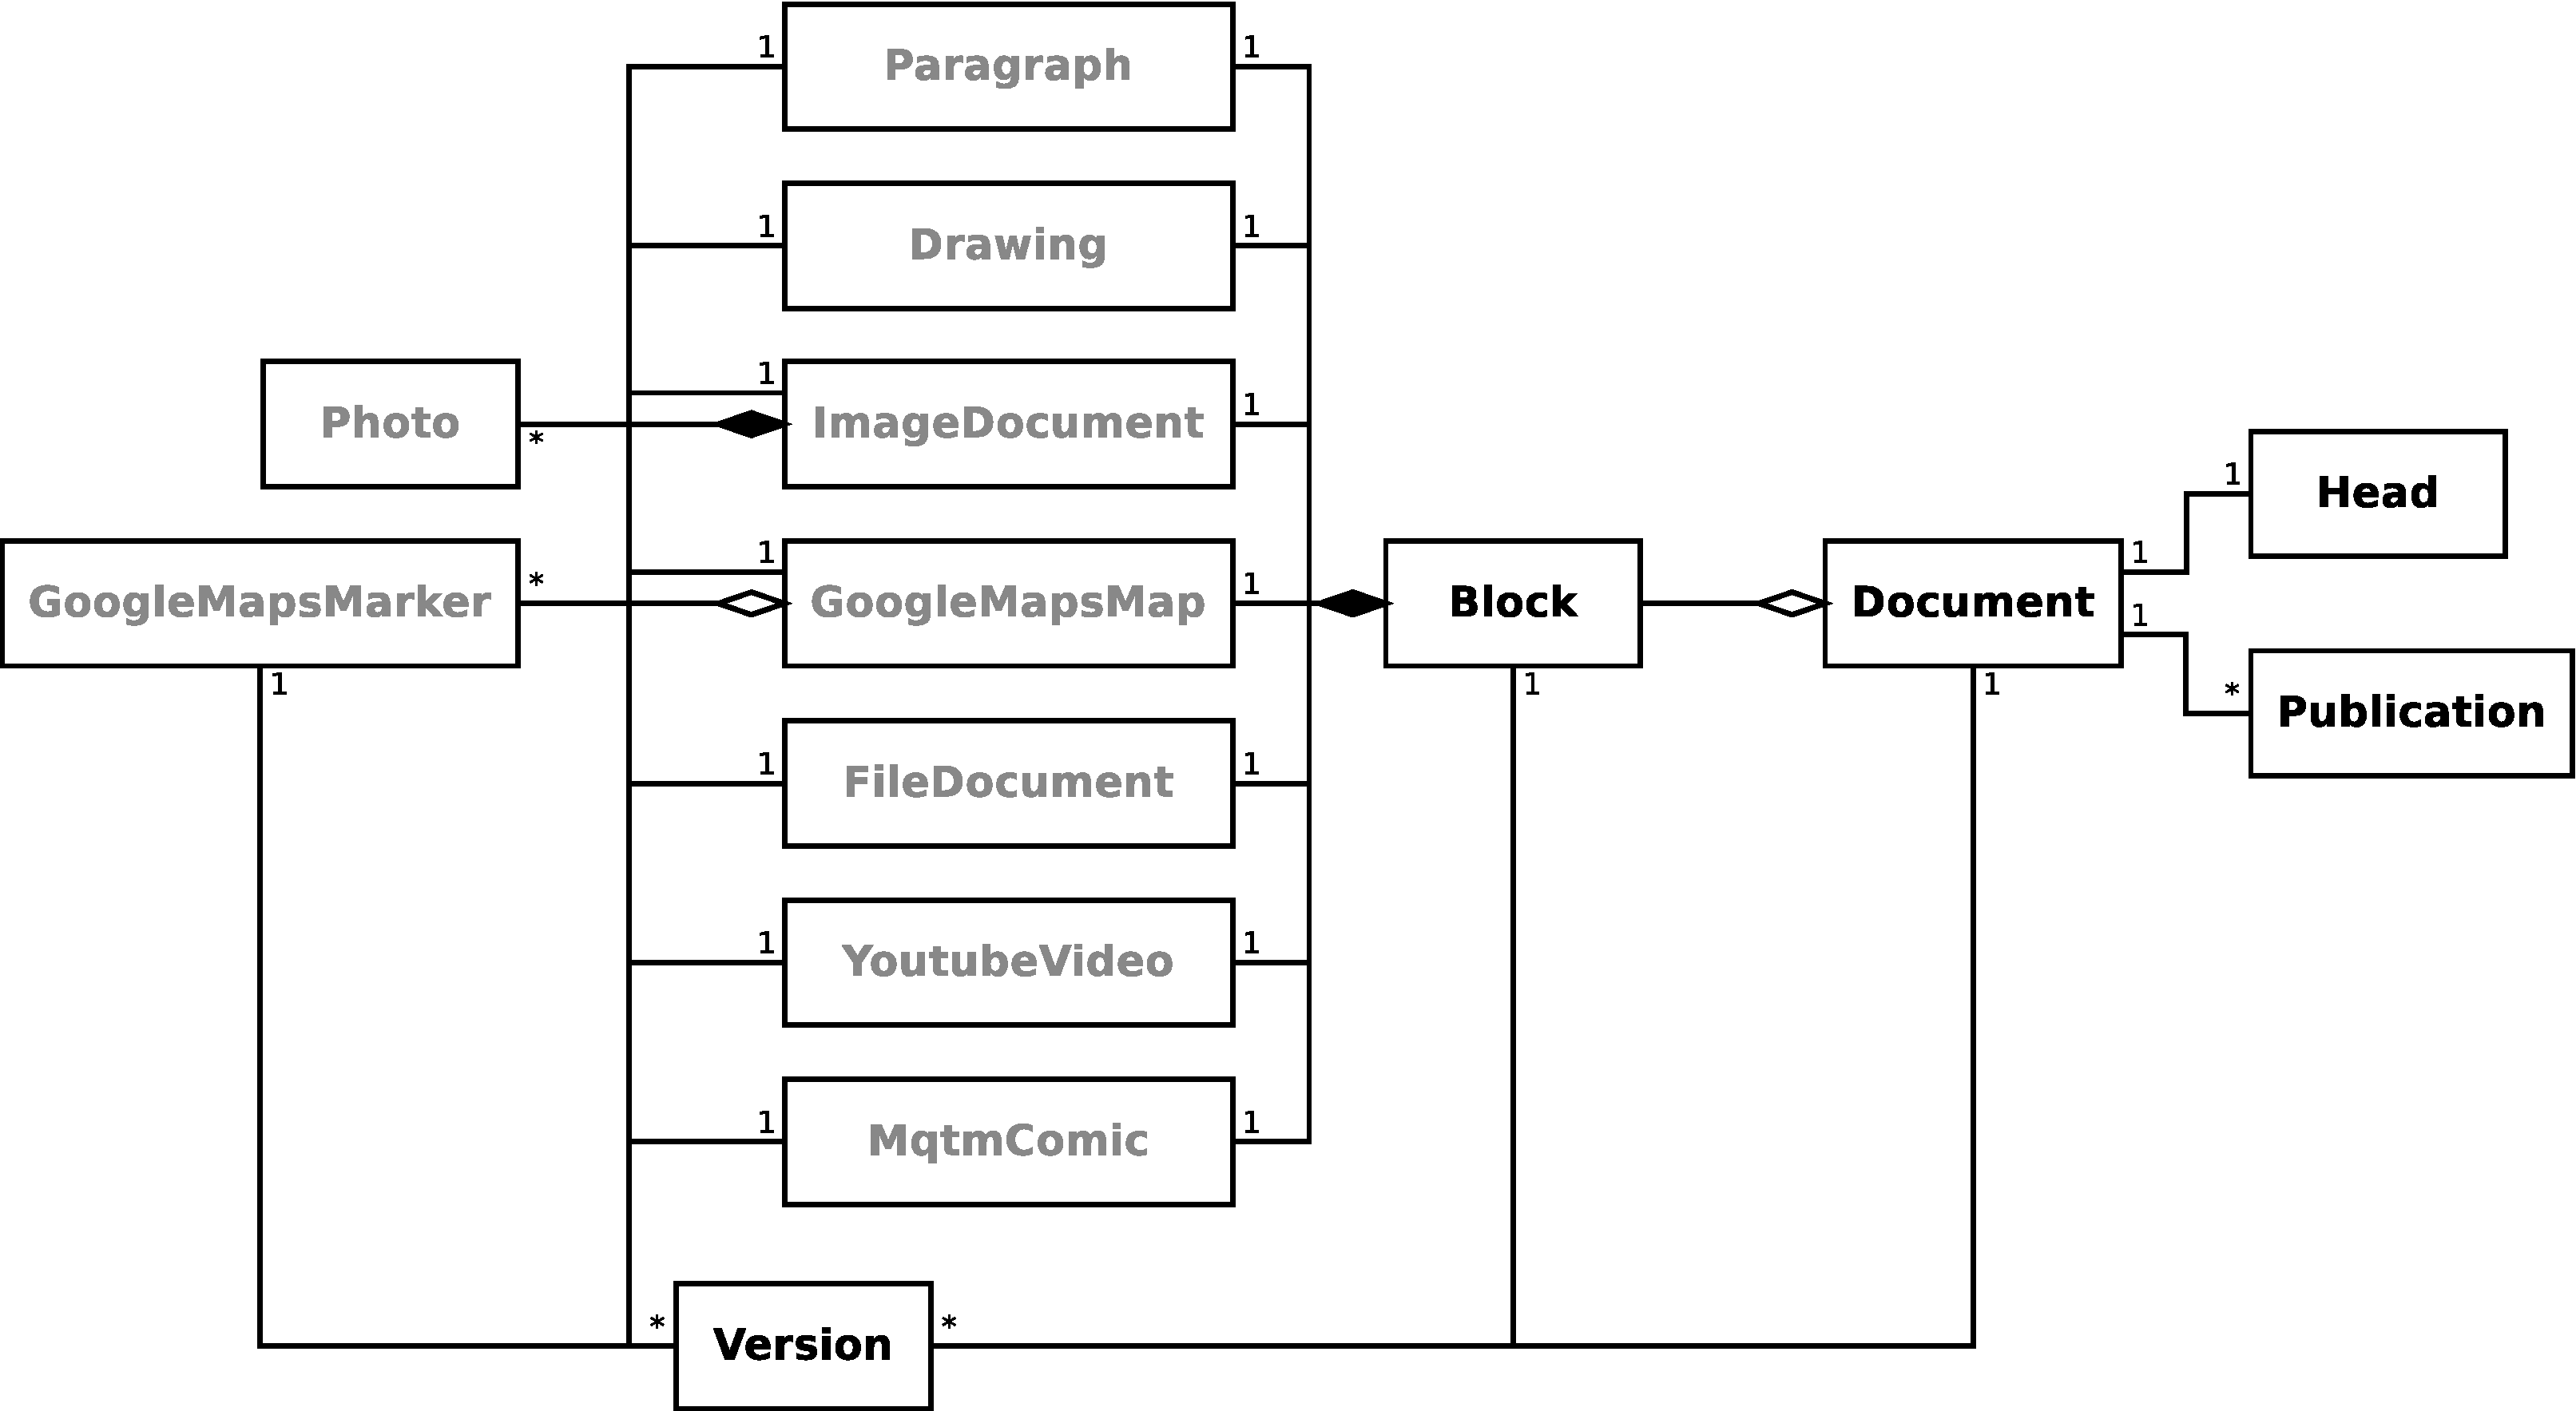
\includegraphics[width=165mm]{documents_current.pdf}
  \caption{Current Documents Model}
  \label{fig:documents_current}
\end{figure}

\subsection{Candidate Patterns}\label{sec:fa_documents_candidate_patterns}

\subsection{Chosen Patterns \& Rationale}\label{sec:fa_documents_chosen_patterns_rationale}

The pattern used is a composite design pattern as described in \cite{riehle_composite_patterns}, where various smaller design patterns work in tandem to create a more complex pattern:

\begin{itemize}
  \item \textsc{Memento} - used for versioning
  \item \textsc{Property} (simplified variant) - used for decoupling a \emph{Block content} from the database schema
  \item \textbf{INVESTIGATE: pattern 3} - the fact that a \emph{Publication} points to a specific \emph{Version} of a \emph{Document} may be a pattern --- it works as a \emph{tag} in a VCS (version control system) system such as git or SVN.
\end{itemize}

\begin{figure}[H]
  \centering
  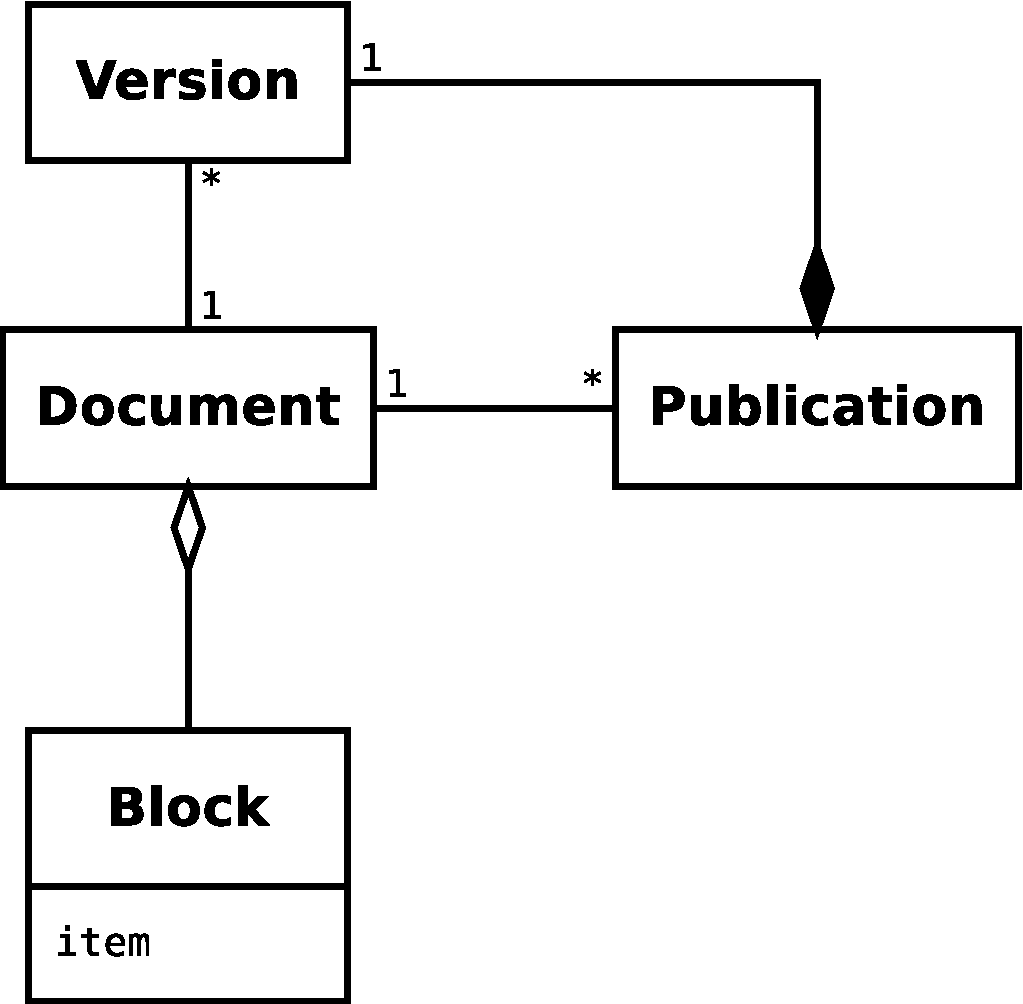
\includegraphics[width=75mm]{documents_conceptual.pdf}
  \caption{Conceptual Documents Model}
  \label{fig:documents_conceptual}
\end{figure}

The variant of the \textsc{Property} pattern implemented is simplified due to the highly dynamic nature of the Ruby language --- which means that, for this particular problem, it is able to build new types of objects or even create new class definitions in runtime, which allows discarding the \textsc{Property}--\textsc{PropertyType} pair (see \ref{sec:property_pattern}) in favour of a single entity, \emph{content}.

\subsection{Implementation}\label{sec:fa_documents_implementation}

The implementation of this composite pattern takes advantage of the highly dynamic nature of the Ruby language and the API provided by the \textsc{ActiveRecord} implementation of Rails.

\emph{Document}, \emph{Block}, \emph{Version} and \emph{Publication} are all AR objects, which means that, according to the AR pattern and the Rails framework conventions, each one of them is stored inside an SQL table, with a row for each one of the attributes. This structure provides the basic blueprint (as stated in \ref{sec:case-study_areas_document_editor}) for the documents to be produced by the editor --- it allows a title, an arbitrary number of orderable blocks, and a snapshot (version) of each modification. It also allows for publications, which essentially point to a specific version of a document.

There is nothing really remarkable about \emph{Blocks}, \emph{Documents} of even \emph{Publications} --- they are ordinary \textsc{ActiveRecord} objects, with associations to each other (as pictured in Fig.~\ref{fig:documents_conceptual}), and explaining how they work is outside of the scope of this study.

However, a \emph{Version} is a bit more complex than a simple AR object, in the sense that it contains a full representation of another AR object at a given point in time --- in this case, a \emph{Document}. This is achieved by serializing a \emph{Document} and all its associations (\emph{Blocks}) in the JSON format, which preserves all the necessary information needed to rebuild a specific \emph{Document} at whichever time that \emph{Version} refers to --- which means that a \emph{Version} effectively implements the \textsc{Memento} design pattern to keep a history of each \emph{Document}.

Finally, a \emph{Block} content possesses special properties that, together with AR, create a dynamic and variable foundation for the development of different types of content. As a \emph{Block} is simply a generic container for an arbitrary type of content, a \emph{Block} content can't be constrained to a single class or object type. The solution is to serialize the content inside the \emph{content} attribute of a \emph{Block}. This way, a \emph{Block} content is simply a string that represents a serialized object --- which can be de-serialized, accessed and modified at runtime. This means that, whichever a \emph{Block} content may be, the content itself is responsible for its representation and life cycle.

In order to further simplify and streamline the development, a \emph{DocumentItem} (super)class was created. This class serves as a staple for further specialization through inheritance, and handles cross-cutting concerns such as object initialization, default values and validations for each of these attribute's values. The need for a specific controller for each one of the different Block items has also been discarded in favour of a single controller, responsible for handling the user input regarding the modification of blocks and their content.

\subsection{Impact Analysis}\label{sec:fa_documents_impact_analysis}

The refactoring of the Document Editor infrastructure had two major points of impact: performance, and variability.


\subsubsection{Performance}

With the current foundation for the editor the number of queries grows linearly with the number of blocks that constitute a document, as it is necessary to perform a query for each one the items related to each one of the blocks. The usage of eager loading is limited due to the polymorphic nature of the blocks and each respective content, which is unknown \emph{a priori}.

From an universe of 3990 documents currently residing in the system (representative of all the documents present in the system as of November 23rd, 2010), the graph present in Fig.~\ref{fig:queries_per_blocks_in_document} shows a linear growth in the number of queries necessary to render a Document: the number of queries necessary are directly proportional to the number of blocks in a document with a 1:1 ratio. Just like in \ref{sec:fa_social_network_impact_analysis}, this represents a serious performance issue: as the most used feature in the \emph{escolinhas.pt} platform, a sustainable growth is very difficult to achieve if the database load increases linearly with the number of existent Documents.

\begin{figure}[H]
  \centering
  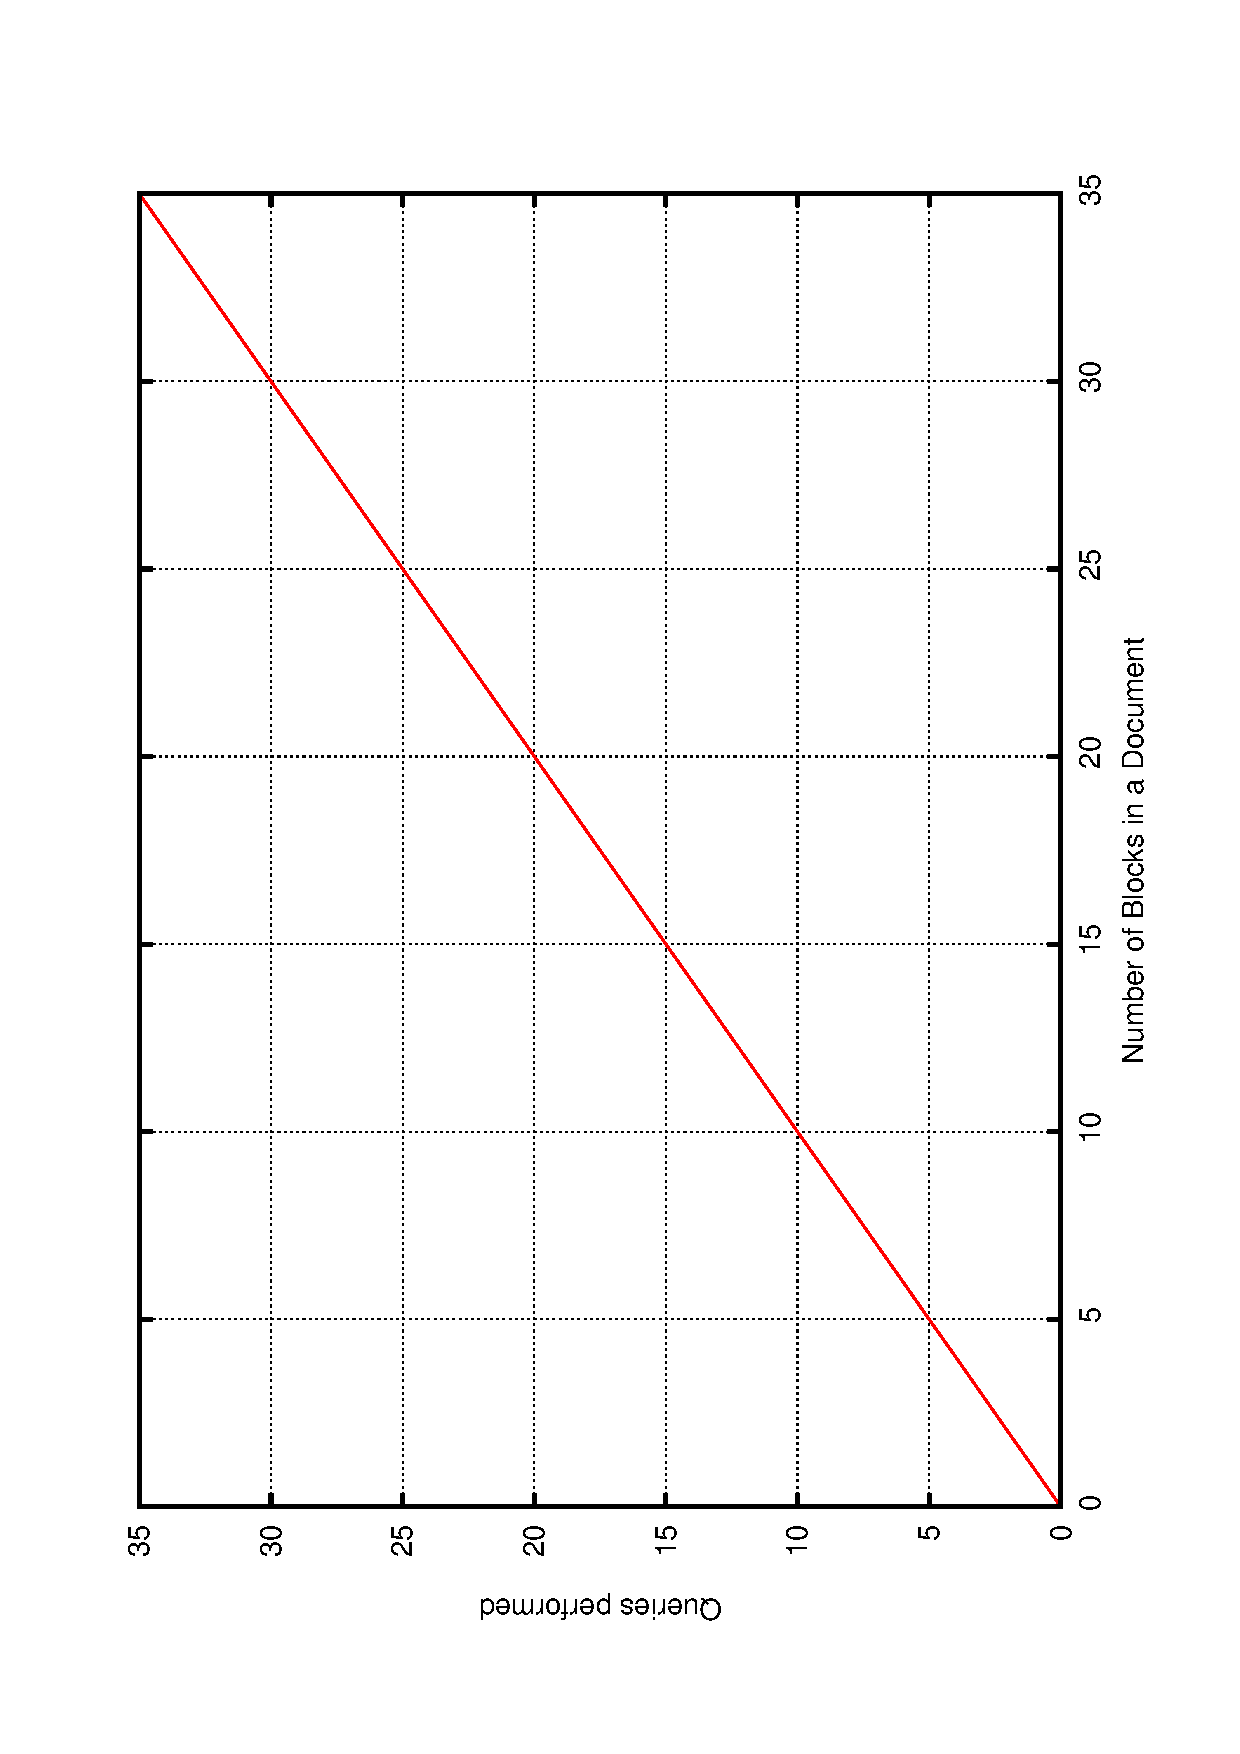
\includegraphics[width=145mm]{document_queries}
  \caption{Number of queries performed per number of Blocks in a single Document}
  \label{fig:queries_per_blocks_in_document}
\end{figure}

The introduction of the model described in \ref{sec:fa_documents_chosen_patterns_rationale} makes the number of queries necessary to display a \emph{Document} to be constant (only 2 queries are performed), as only the Blocks and the Document itself are AR objects --- as the item that constitutes a Block is an integral part of a Block, no queries are necessary to fetch it.

\subsubsection{Variability}

With the introduction of this model, the work necessary to create new types of blocks has been greatly reduced. This allows for much shorter prototyping and testing iteration times --- no database schemas or migrations to worry about, allowing the developers to focus on the details of the model rather than implementation details --- which ultimately leads to a higher degree of variability.










\chapter{Validation}\label{chap:validation}

\chapter{Conclusion}\label{chap:conclusion}

The problem described in chapter \ref{chap:problem_statement} has been solved according to the solution presented in chapter \ref{chap:approach_results} and the results achieved from this approach have been presented in the same chapter. In this last chapter, Section \ref{sec:conclusions}, some last remarks will be made about this study, as well as a summary of the main achievements and results. In Section \ref{sec:further_developments} the further improvements to the project will be presented and in Section \ref{sec:future_works} the future works will be described.

\section{Conclusions}\label{sec:conclusions}

Despite being built with a MVC architecture, the Ruby On Rails framework is, using the right approach, capable of working with some architectural and design patterns not obviously connected with MVC and AR. The application of these patterns is capable of increasing the level of variability present in a common Rails application, and a harmonious integration with the Rails 2.3.x infrastructure --- especially the \textsc{ActiveRecord} engine --- is possible and works elegantly.

Although the majority of the work present in this thesis in concerned with increasing the variability of software systems, it is possible to conclude that the application of the appropriate design patterns is able to increase not only the variability and configurability needs of a specific part of an application, but also its performance. However, this should not be taken as an universal truth, as it depends on a series of factors that may not be present in all implementations, such as a previous innapropriate design.

\section{Further Developments}\label{sec:further_developments}

The main improvements and additions that can be made to the final work presented are divided into 2 groups:

\begin{itemize}
 \item Implement everything!
 \item Keep the accountabilities in memory
\end{itemize}

\section{Future Works}\label{sec:future_works}

In this section it will be discussed the projects that can be derived from this study as well as the applications and domains that can be dealt using the same methodological approach.

 * Test integration of these pattern with Rails 3

%Adaptive Object-Model architectures provide the best framework for building adaptable systems that are passable of modification by the end-users (which assumes no compilation or deployment processes). A lot of thought and research has gone into the best practices for the complete implementation of these types of systems, from model creation, maintenance and persistence to GUI generation.

%There has been very few work regarding true adaptive systems on the web. However, a considerable amount of research has been made regarding the best mechanisms for end-user website customization, which can be used to create web applications based on AOM architectures. 


%%----------------------------------------
%% Final materials
%%----------------------------------------

\begin{singlespace}
  %% Bibliography
  %% Comment the next command if BibTeX file not used,
  %% bibliography is in ``myrefs.bib''
  \PrintBib{thesis}

  %% Index
  %% Uncomment next command if index is required,
  %% don't forget to run ``makeindex mieic'' command
  %\PrintIndex

  %% Comment next 2 commands if numbered appendixes not used
  \appendix
  \chapter{Loren Ipsum} \label{ap1:loren}

Depois das conclusões e antes das referências bibliográficas,
apresenta-se neste anexo numerado o texto usado para preencher a
dissertação.

\section{O que é o \emph{Loren Ipsum}?}

\emph{\textbf{Lorem Ipsum}} is simply dummy text of the printing and
typesetting industry. Lorem Ipsum has been the industry's standard
dummy text ever since the 1500s, when an unknown printer took a galley
of type and scrambled it to make a type specimen book. It has survived
not only five centuries, but also the leap into electronic
typesetting, remaining essentially unchanged. It was popularised in
the 1960s with the release of Letraset sheets containing Lorem Ipsum
passages, and more recently with desktop publishing software like
Aldus PageMaker including versions of Lorem Ipsum~\citep{kn:Lip08}. 

\section{De onde Vem o Loren?}

Contrary to popular belief, Lorem Ipsum is not simply random text. It
has roots in a piece of classical Latin literature from 45 BC, making
it over 2000 years old. Richard McClintock, a Latin professor at
Hampden-Sydney College in Virginia, looked up one of the more obscure
Latin words, consectetur, from a Lorem Ipsum passage, and going
through the cites of the word in classical literature, discovered the
undoubtable source. Lorem Ipsum comes from sections 1.10.32 and
1.10.33 of ``de Finibus Bonorum et Malorum'' (The Extremes of Good and
Evil) by Cicero, written in 45 BC. This book is a treatise on the
theory of ethics, very popular during the Renaissance. The first line
of Lorem Ipsum, ``Lorem ipsum dolor sit amet\ldots'', comes from a line in
section 1.10.32.

The standard chunk of Lorem Ipsum used since the 1500s is reproduced
below for those interested. Sections 1.10.32 and 1.10.33 from ``de
Finibus Bonorum et Malorum'' by Cicero are also reproduced in their
exact original form, accompanied by English versions from the 1914
translation by H. Rackham.

\section{Porque se usa o Loren?}

It is a long established fact that a reader will be distracted by the
readable content of a page when looking at its layout. The point of
using Lorem Ipsum is that it has a more-or-less normal distribution of
letters, as opposed to using ``Content here, content here'', making it
look like readable English. Many desktop publishing packages and web
page editors now use Lorem Ipsum as their default model text, and a
search for ``lorem ipsum'' will uncover many web sites still in their
infancy. Various versions have evolved over the years, sometimes by
accident, sometimes on purpose (injected humour and the like). 

\section{Onde se Podem Encontrar Exemplos?}

There are many variations of passages of Lorem Ipsum available, but
the majority have suffered alteration in some form, by injected
humour, or randomised words which don't look even slightly
believable. If you are going to use a passage of Lorem Ipsum, you need
to be sure there isn't anything embarrassing hidden in the middle of
text. All the Lorem Ipsum generators on the Internet tend to repeat
predefined chunks as necessary, making this the first true generator
on the Internet. It uses a dictionary of over 200 Latin words,
combined with a handful of model sentence structures, to generate
Lorem Ipsum which looks reasonable. The generated Lorem Ipsum is
therefore always free from repetition, injected humour, or
non-characteristic words etc. 

\end{singlespace}

\end{document}

